\documentclass[12pt, a4paper, colorinlistoftodos]{article}


\usepackage{soul}
\usepackage{natbib}
\usepackage{hyperref}
\usepackage{bookmark}
\usepackage{graphicx}             
\graphicspath{{./Figuras/}}

\usepackage{makecell}
\usepackage[margin=1in]{geometry}
\usepackage{float}                
\usepackage{amsmath}
\usepackage{amscd}
\usepackage{amsfonts}
\usepackage{amssymb}
\usepackage{bbm}
\usepackage{booktabs}
\usepackage{nameref}
\usepackage{multirow}
\usepackage[nokeyprefix]{refstyle}
\usepackage{rotating}
\usepackage{threeparttable}
\usepackage{afterpage}
\usepackage{lscape}
\usepackage{enumerate}
\usepackage{caption}
\usepackage{subcaption}
\usepackage{epstopdf}
\usepackage{setspace}
\usepackage{svg}
\usepackage{dsfont}
\usepackage{amsthm}
\usepackage{tocloft}
\usepackage{etoc}
\usepackage{lmodern}
\usepackage{bm}

\epstopdfDeclareGraphicsRule{.tiff}{png}{.png}{convert #1 \OutputFile}
\AppendGraphicsExtensions{.tiff}

\epstopdfDeclareGraphicsRule{.tif}{png}{.png}{convert #1 \OutputFile}
\AppendGraphicsExtensions{.tif}

\usepackage{tikz}
\usetikzlibrary{shapes.geometric, arrows}
\usetikzlibrary{calc}
\usetikzlibrary{matrix}

\tikzset{ 
    table/.style={
        matrix of nodes,
        row sep=-\pgflinewidth,
        column sep=-\pgflinewidth,
        nodes={
            rectangle,
            draw=black,
            align=center
        },
        minimum height=1.5em,
        text depth=0.5ex,
        text height=2ex,
        nodes in empty cells,
%%
        every even row/.style={
            nodes={fill=gray!20}
        },
        column 1/.style={
            nodes={text width=2em,font=\bfseries}
        },
        row 1/.style={
            nodes={
                fill=black,
                text=white,
                font=\bfseries
            }
        }
    }
}


\usepackage{colortbl}

\newtheorem{theorem}{Theorem}
\newtheorem{claim}[theorem]{Claim}
\newtheorem{prop}[theorem]{Proposition} 
\newtheorem{cor}[theorem]{Corollary} 

\DeclareRobustCommand{\hlgr}[1]{{\sethlcolor{green}\hl{#1}}}


\usepackage{comment}
%para esconder columnas en tablas (enrique)
\usepackage{array}
\newcolumntype{H}{>{\setbox0=\hbox\bgroup}c<{\egroup}@{}}
\linespread{1.25}

\newcommand{\wh}{\widehat}
\usepackage{anyfontsize}

\usepackage[linesnumbered,vlined,ruled,commentsnumbered]{algorithm2e}

\DontPrintSemicolon
\newcommand{\To}{\mbox{\upshape\bfseries to}}

%%% HELPER CODE FOR DEALING WITH EXTERNAL REFERENCES
\usepackage{authblk}
\makeatletter
\renewcommand\AB@affilsepx{, }
\makeatother
\renewcommand\Authands{ and }
\renewcommand\Affilfont{\small}
\setlength{\affilsep}{0em}
\usepackage{xr}
\makeatletter
\newcommand*{\addFileDependency}[1]{
  \typeout{(#1)}
  \@addtofilelist{#1}
  \IfFileExists{#1}{}{\typeout{No file #1.}}
}
\makeatother


\newcommand*{\myexternaldocument}[1]{
    \externaldocument{#1}
    \addFileDependency{#1.tex}
    \addFileDependency{#1.aux}
}

\newgeometry{margin=1in}
\linespread{1.25}

% To-do commands (must go after authblk to avoid clash)
\usepackage{todonotes}
\usepackage{marginnote}
\renewcommand*{\marginfont}{\color{red}\sffamily\scriptsize}
\setlength{\marginparwidth}{2cm}  % prevent todo cutoff
\newcounter{todoListItems}
\newcommand{\todoLink}[2][ ]{
  \addtocounter{todoListItems}{1}
  \todo[caption={\protect\hypertarget{todo\thetodoListItems}{}Translation},size=\tiny,#1]{
    \tiny #2 \hfill \hyperlink{todo\thetodoListItems}{$\uparrow$}
  }
}
\newcommand{\forES}[1]{\todoLink[color=green!20,inline,caption={\thetodoListItems: For @Enrique}]{\textbf{@Enrique} -- #1}}
\newcommand{\forIM}[1]{\todoLink[color=blue!20,inline,caption={\thetodoListItems: For @Isaac}]{\textbf{@Isaac} -- #1}}
\newcommand{\forFdT}[1]{\todoLink[color=red!20,inline,caption={\thetodoListItems: For @Francis}]{\textbf{@Francis} -- #1}}
\newcommand{\forCM}[1]{\todoLink[color=violet!20,inline,caption={\thetodoListItems: For @Craig}]{\textbf{@Craig} -- #1}}
\newcommand{\forAll}[1]{\todoLink[color=orange!20,inline,caption={\thetodoListItems: For All}]{\textbf{@All} -- #1}}

\begin{document}

\listoftodos

\title{Structured Payment in Pawnshop Borrowing: Mandates vs.\ Choice\thanks{We thank Jose Maria Barrero, Camilo García-Jimeno, Andrei Gomberg, Emilio Gutierrez, Anett John, David Laibson, Aprajit Mahajan, Matt Rabin, Mauricio Romero, Charlie Sprenger, Séverine Toussaert, Chris Udry, Jonathan Zinman, and seminar participants at Dartmouth, ITAM, MSU, USC, UC Davis, UCSD, and USC who provided valuable feedback. Ricardo Olivares, Gerardo Melendez, and Alonso de Gortari provided excellent research assistance and Erick Molina helped with formatting.  Research assistance was financed through faculty grants at ITAM. Our research partner had no say in the design or results of the experiment.}}
\author[1]{Francis J.\ DiTraglia}
\author[2]{Craig McIntosh}
\author[3]{Isaac Meza}
\author[4]{Joyce Sadka}
\author[5]{Enrique Seira\thanks{Corresponding Author: \href{mailto:enrique.seira@gmail.com}{enrique.seira@gmail.com}}}
\affil[1]{\normalsize University of Oxford} %\href{mailto:francis.ditraglia@economics.ox.ac.uk}{francis.ditraglia@economics.ox.ac.uk}}
\affil[2]{\normalsize University of California San Diego}
%\href{mailto:ctmcintosh@ucsd.edu}{ctmcintosh@ucsd.edu}}
\affil[3]{\normalsize Harvard University}
%\href{mailto:isaacmezalopez@g.harvard.edu}{isaacmezalopez@g.harvard.edu}}
\affil[4]{\normalsize ITAM}
%, \href{mailto:jsadka@itam.mx}{jsadka@itam.mx}}
\affil[5]{\normalsize University of Notre Dame}


\date{\today \\[2 cm]}


%\vspace{.5in}


\maketitle
\vspace{-0.75in}

\begin{abstract}
%We explore the merits of structured repayment contracts in the understudied context of pawn lending. We use a novel one-stage, three-armed RCT, including mandatory and voluntary treatment arms, to point-identify the effects of regular monthly payments both for individuals who would freely choose, and would not freely choose, structured payments. We find that assigning borrowers to commitment-style contracts decreases the financial cost of pawn loans by 22\% and increases the likelihood of recovering their pawn by 15\%. However, only 11\% of borrowers choose such contracts voluntarily. We find that borrowers who would \textit{not} choose regular payments would benefit substantially from getting such contracts, as much as those freely choosing them (no selection on gains).  A paternalistic policy mandating structured payments helps a sufficiently large fraction of borrowers that it cannot be improved upon by feasible personalized targeting. 
\singlespacing
Pawn loans offer borrowers a high degree of repayment flexibility in exchange for a harsh penalty in case of default: forfeit of collateral worth more than the loan amount. Using a large RCT conducted in Mexico City, we document key stylized facts and explore the merits of replacing flexibility with structured repayment contracts in this important but understudied form of credit. 
A novel experimental design that includes a mandatory frequent-payments arm, a (status quo) flexible payments arm, and a choice between the two, point-identifies not only the average treatment effect, but also the effects of treatment on the treated and the untreated along with the average selection on gains, allowing a rigorous study of mandates versus choice. Although the average treatment effect of assigning borrowers to structured payments is a 22\% decrease in their financial cost and a 15\% increase the probability that they will recover their pawn, only 11\% of borrowers choose structured repayment contracts voluntarily. We show that structured repayment benefits nearly all borrowers, including those who would not freely choose it, and find no evidence of selection on gains. 
%Nonetheless, lenders' profits are lower under structured payments since they earn more from borrower default, giving lenders little incentive to offer such contracts. 

\end{abstract}

%\vspace{.6in}
\noindent \textbf{Keywords: } Mandates versus choice, paternalism, treatment on the untreated, payment frequency, overconfidence.\\ \textbf{JEL codes:} G41, C93, O16, G21


%%%%%%%%%%%%%%%%%%%%%%%%%%%%%%%%%%%%%%%%%%%%%%%%%%%%%%%%%%%%%%%%%%%%%%%%%
%%%% Main text entry area:
%%%%%%%%%%%%%%%%%%%%%%%%%%%%%%%%%%%%%%%%%%%%%%%%%%%%%%%%%%%%%%%%%%%%%%%%%

\newpage

\section{Introduction}

\forES{Enrique please do this}

\forIM{Please that}

Pawn lending is one of the oldest and most prevalent forms of credit in the world \citep{carter2012pawnshops}. Pawn loans are typically small, and short-term. They involve no credit checks or proof of income, and are widely used by people without access to other forms of credit. Borrowers surrender highly liquid collateral as the pawn, typically gold, in return for a loan that is substantially smaller than their pawn's value.  These loans are very flexible: there are no scheduled payments, no prepayment penalties, and interest is charged only on outstanding balance. Unlike mortgage lenders, pawn lenders retain the entire value of the collateral under default along with any payments already made, rather than simply recovering the outstanding value of the loan.  There are more than 11,000 pawn shops across the US with 30 million clients and \$14 billion yearly revenues; in China pawn lending is a 43 billion dollar industry.\footnote{\url{https://tinyurl.com/ybm56dpe}, \url{https://tinyurl.com/y9zdcgws}, \url{https://tinyurl.com/y59ptdam}. In Mexico the scale of pawn lending rivals that of microfinance: during the past three years a single large lender in the country made over 4 million loans to more than a million clients, compared to a total of 2.3 million microfinance clients in all of Mexico during 2009 \citep{Pedroza:2010}.}  Despite this, pawnshops have received little attention in the literature to date. 

Pawn loans are different from conventional credit in important ways. First, pawn loans typically default at much higher rates than other forms of credit. For example, 44\% of loans made by our partner lender are not repaid, and 29\% of those who fail to repay make payments prior to defaulting, money which is completely lost to them subsequently. Second, lender profits are higher under default than repayment. An industry standard contract in Mexico City lends 70\% of the value of gold collateral at an interest rate of 7\% for three months. Because gold is highly liquid, the profit from a borrower who defaults is 30\% of the collateral value compared to 22.5\% in interest if a loan is paid in full on the last day.   Furthermore, pawn borrowers are typically economically vulnerable and, in our context, are also naively optimistic; borrowers report a subjective probability of repayment that averages 92\%. The unusual degree of flexibility in these contracts would benefit borrowers if they were neo-classical agents, but the prevalence of costly default that hurts borrowers but benefits lenders, combined with apparently naive borrowers, calls this into question. Other lending modalities with dramatically lower equilibrium default, such as microfinance, typically rely on highly structured repayment regimes.
%Hence pawn lending features unusual dynamics, and lender incentives are quite different from other forms of lending.


%Much of the literature on standard credit contracts has illustrated that structured repayment schedules help borrowers avoid default \citep{morduch1999microfinance}.  Indeed, \cite{Laibson2018} has discussed the many ways in which forcing devices like structure and deadlines are embedded into schools, workplaces, and financial institutions so as to improve outcomes whether or not the customers would have freely elected these features.  Pawn lending, in contrast with the highly structured contracts of microfinance lending, typically features no reminders or regular payment schedule, with borrowers required to remember to make a single balloon payment withing the contracted time or else lose the pawn.  Given this combination of issues, it appears possible that the lack of structure in pawnshop lending is strategic on the part of lenders.  This raises the possibility of potential gains to borrowers by introducing contracts with more regularized repayment structure.  


%Financial institutions often use built-in commitment mechanisms like fixed repayment streams to lower default rates and increase their own profits. At the same time, they frequently ``shroud'' these attributes by embedding them as non-negotiable features of the loan contract, presumably because borrowers undervalue commitment and would not demand it, given the choice. \cite{Laibson2018} refers to this practice as ``private paternalism''. When the incentives of firm and client align, as they do in \cite{Laibson2018}, private paternalism can benefit both parties. Pawn lending, however, turns this idea on its head: since the value of the collateral--the pawn--exceeds that of the loan, lenders stand to gain the most when borrowers default.Consistent with this idea, and in stark contrast to microfinance, pawn lenders in Mexico City neither send payment reminders to borrowers nor provide commitment features in their contracts. Default is common.\footnote{The default rate in the \emph{status quo} arm of our Mexico City experiment is 44\%.} 

This paper asks whether structured repayments can help pawnshop borrowers avoid default.  To do so, we present a unique three-armed experiment covering around 4,500 pawnshop clients across six of our partner lender's Mexico City branches.  Borrowers in the Control arm received the standard status quo pawn contract (described above) which allows us to document payment trajectories and default in standard pawn markets.  Borrowers in the `Structured' arm were required to make three monthly payments, with each monthly payment including the accrued interest at that time, and faced a nominal fee of 2\% of that month's payment if the payment was delinquent.  Borrowers in the `Choice' arm were allowed to choose between the Standard and Structured contracts.   A design that features both assignment and choice permits a nuanced understanding of how treatment effects relate to the choices that individuals freely make: because our context featured no differential selection of clients across arms, we can recover a unique combination of economically-relevant causal estimands.\footnote{See Section \ref{sec:integrity} for details.}


Comparing the Structured and Control arms gives the Average Treatment Effect (ATE) of structured repayment in the pawnshop context.  Comparing the Choice arm to the Control provides a standard Intention to Treat (ITT) effect of offering this option.  The presence of all three arms in the same experiment then allows us to point identify treatment effects \emph{separately} for those who would and would not choose structure, given the choice.  Consider only the Control and Choice arms. No one in the Control arm is treated, but some borrowers in the Choice arm choose to be treated: choosers. We can view the comparison of these two arms as an experiment with one-sided non-compliance. Here assignment to the choice arm serves as an instrumental variable for treatment receipt. Under an exclusion restriction, a familiar argument shows that the IV estimator identifies the causal effect for people who are shifted by the instrument: choosers. This is the Treatment on the Treated (TOT).  Now consider only the Choice and Structured arms. Everyone in the Structured arm is treated, but some borrowers in the Choice arm choose not to be treated: non-choosers. We can view the comparison of these two arms as a separate experiment, also with one-sided non-compliance. Here assignment to the Structured arm serves as an instrumental variable for treatment receipt. Under a symmetric exclusion restriction, an almost identical argument shows that the IV estimator identifies the causal effect for people who are shifted by the instrument: non-choosers. This is the Treatment on the Untreated (TUT).  As far as we are aware, this is the only experimental paper that provides a direct comparison of the TUT and TOT in the same context.  This comparison is key for studying voluntary versus mandatory treatment.

%\todo[inline]{Should add a bit more on the ``mandates versus choice'' design here, including some other possible scenarios where it could be employed: education experiment, 401k, online privacy settings.}

This design reveals critical information about marginal treatment effects and selection on gains, and is useful for any circumstance in which we want to compare voluntary versus mandated compliance.  In educational settings, it may be useful to understand whether providing optional exercises in advance of a major exam is sufficient, or whether it is more effective to require students to complete these.  In the much-studied context of employer-based retirement savings plans, this design can be used to examine the relative benefits of providing options for higher and earlier employee contributions versus simply defaulting employees into more aggressive savings plans.  Digital service providers trying to understand how digital privacy settings drive platform engagement and monetization could either provide choices to consumers or simply default them into stricter protections, and our design provides a way of comparing the relative benefits of these approaches.  In general, our method for testing the TOT against the TUT provides a practical way of understanding how treatment effect heterogeneity relates to real-world compliance decisions.


%while comparing.  Invoking the standard exclusion restriction, we can calculate the Treatment on the Treated (TOT) for choosers in the Choice arm.  Novel to this context is that we can then use a symmetric assumption to calculate the Treatment on the Untreated (TUT) by comparing the Choice and Assigned arms to each other.  Thus, in a single context and with minimal assumptions, this design allows us to compare the treatment effects for individuals who would have and would not have freely chosen the treatment.  %We provide Stata code to conduct correct inference on the comparison of the TOT and the TUT, which is the relevant comparison for any applied policy conversation about the relative benefit of offering a policy versus imposing it upon agents.
%\textcolor{teal}{We explain in the paper why the estimation of TUT is essential to assess the pros and cons of mandating a contractual feature (in our lexicon, imposing a mandate and eliminating choice is a form of paternalism).}

%ompared to the status quo arm that continues to receive the standard pawn contract, we that answers three key questions. First, does the absence of commitment-style contracts cause default in pawn lending? If so, to what extent does this benefit lenders? Second, if a commitment contract were available would pawn borrowers choose it? Even more importantly, would the \emph{right} borrowers choose it, i.e.\ those who would benefit the most? Third, is there a case for \emph{paternalism}, namely for mandating commitment in pawn lending? If so, should commitment be mandated for all borrowers or can it be effectively targeted? The question of choice versus paternalism is particularly salient in a setting with vulnerable borrowers. Yet comparing voluntary versus paternalistic policies is challenging. Even if commitment lowers financial costs on average, it may be ineffective or even harmful for borrowers who \emph{would not choose} to commit. To meet this challenge we introduce a novel three-armed design, the ``forcing-choice'' design, that allows us to shed light on these three questions in the important and under-studied context of pawn lending. 

%Our experiment covers just under 5,000 pawnshop clients across six of our partner lender's Mexico City branches. The control arm illustrates the costs of the \emph{status quo} contract: fully 44\% of control borrowers default, losing their pawn along with any payments made towards principal. Worse still, 29\% of those who default do so after making at least one payment towards recovery, a payment that they forfeit upon default. The ``forced commitment'' arm requires borrowers to make three monthly payments, with each monthly payment including the accrued interest at that time as well as a nominal fee of 2\% of that month's payment if the payment is delinquent.  Finally, the ``commitment choice'' arm offers borrowers the chance to opt in to the same structured monthly contract that is mandated for borrowers in the forced commitment arm.\footnote{When describing this new contract below, we use the terms ``commitment'' and ``structured payment'' interchangeably.}

%Because there is no selection into or out of the control (status quo) and forced commitment arms in our experiment, the forcing-choice design can be viewed as a \emph{juxtaposition} of three more familiar experimental designs.\footnote{See section \ref{sec:integrity} for a discussion of how we can be sure that there was no selection into or out of the treatment and forced commitment arms.} The first is a standard two-armed RCT with perfect compliance that point identifies the average treatment effect (ATE) of commitment. The other two are a pair of randomized encouragement designs, each with one-sided non-compliance: one point identifies the effect of commitment for borrowers who would \emph{voluntarily} choose commitment (treatment on the treated: TOT), while the other point identifies the effect of commitment for borrowers who would \emph{not} (treatment on the untreated: TUT). Fully evaluating the case for paternalism versus borrower choice requires policymakers to learn not only whether those who demand commitment benefit from it (TOT), but also whether those who \emph{do not} are better off without it (TUT).


Our ATE results show that mandatory structured payments are strongly effective in lowering financial costs to borrowers and preventing default in pawnshop lending: the average borrower in the Structured arm pays financing costs inclusive of fees that are 22\% lower than the control, and faces a probability of default that is 6.6 percentage points lower (15\% of the mean). In terms of Annual Percentage Rates (APR), the financial cost of borrowing falls by 11 percentage points per loan (19\% of the mean). In short, structured repayment saves borrowers money by charging them fees. The mechanism by which our monthly payment contract achieves these cost savings is intriguing: not only does it improve repayment and speed up the pace of payments on average, but it also decreases the amount of money paid by borrowers who will ultimately go on to default. While we find that borrowers who experience structured payment contracts are 6 percentage points more likely to borrow again from the same lender, a back-of-the-envelope calculation suggests that the structured contract nevertheless lowers lender profits by at least 14\% per borrower. It is thus unsurprising that structured payment contracts were unavailable in Mexico city pawnshops outside of our experiment: lenders profit from default.\footnote{Unlike most pawn lenders, our partner operates as a non-profit, donating all of their earnings to philanthropic causes.}

%Given the limited measures that are available to us, we refrain from making definitive welfare statements in this paper, focusing instead on the cost of loan servicing, an important outcome in credit markets.\footnote{\hl{Enrique will find citations for a defensive footnote that goes here, pointing out that lots of papers use this as an outcome measure.}} Nevertheless, we explore the sensitivity of our findings to broader notions of cost. For example, our results are qualitatively robust to deducting transport costs of visiting the branch to make interim payments along with a day of lost wages for each visit. They are also robust to using borrowers' \emph{subjective} values of their pawns rather than the appraised value and to adjusting for lost liquidity from requiring monthly payments.  


Despite the large financial cost savings that it provides, there is low demand for structured repayment: only 11\% of borrowers in the choice arm choose structure. The mystery is then why so few people choose a contract that is financially beneficial on average.  Could it be that this small fraction of ``choosers'' simply represents the only individuals who benefit from structure?  The strongly significant difference between the Structured arm and the Choice arm suggests that this is not the case.  More rigorously, an exercise that non-parametrically bounds the distribution of individual treatment effects, following \cite{fan2010sharp}, shows that structured repayment benefits more than twice the number of people who chose it, even under the most conservative assumptions. Imposing the two exclusion restrictions \hl{mentioned above} \forFdT{We did not mention them above} allows us to go further, point identifying the average treatment effects for choosers (TOT) and non-choosers (TUT) along with the average selection on gains ($\text{ASG} = \text{TOT} - \text{TUT}$), a measure of the empirical relevance of Roy-type selection.  Our estimated TOT implies that choosers actually see a very small and insignificant increase in the cost of their loans from structure. \forCM{FC is not that small} The TUT effect, in contrast, suggests that the financial cost savings to non-choosers are large: \$192 pesos, equivalent to a 10.6 percentage point savings in APR. On average, the borrowers who would \emph{not} choose commitment, would have faced substantially lower financial costs if they had. We find no evidence of selection on gains. Finally, we combine our experimental treatment and outcome data with survey responses collected for a subset of borrowers to estimate conditional average treatment effects, both TUTs and ATEs, using the Causal Random Forest algorithm of \cite{atheygrf}. We estimate positive conditional average TUT effects for 93\% of the borrowers who did \textit{not} choose the structured contract. In short, it is extremely difficult to find identifiable groups of borrowers who incur higher financial costs under a structured contract, even when restricting attention to those who would not choose it voluntarily


%The question that our design allows us to address is then whether the \textit{right} people selected into the structured contract, based on the treatment effects observed.  To answer this question, and to think very carefully about the implications of imposing structure when some borrowers could be hurt by it, we carry out a detailed analysis of treatment effect heterogeneity.We begin by bounding the distribution of individual treatment effects using the marginal outcome distributions from Assigned commitment and Control arms, following \cite{fan2010sharp}. 
%This approach imposes no assumptions beyond the experimental randomization. We find that \emph{at least} 23\% of borrowers benefit from the structured payment contract. This implies that there must be many borrowers in the choice arm who did not demand this feature despite their \emph{individual treatment effect} from (assigned) commitment being positive. 





%This is a relatively common if often implicit assumption in causal inference.\footnote{Papers that use variation in compulsory schooling laws to identify the returns to schooling, for example, typically interpret their results as the causal effect of additional \emph{education} rather than additional \emph{forced education}. \cite{chamberlain2011bayesian} uses a closely related assumption to develop a theory of optimal treatment choice.} 
%It also has testable implications that we fail to reject in our empirical context.\footnote{See\autoref{sec:testing_exclusion} \hl{for details--Frank will move some of this into the body of the text.}}

So why do borrowers seem to be leaving money on the table?
One possible explanation could be impatience: under a standard model of rational choice, a sufficiently impatient borrower might prefer the status quo contract in spite of the higher probability of default.
%; our measures of profit are not discounted, and so could a sufficiently impatient borrower prefer the status quo contract? 
We find, however, that discount rates of almost 4,000\% would be required to rationalize such a preference, making impatience an unlikely explanation for the low take-up of structured repayment contracts. Another potential explanation frequently raised in the literature is time inconsistency: hyperbolic borrowers might choose a contract that maximizes short-term liquidity.  We find that a standard survey measure of time inconsistency does not predict larger TUT effects while pawn recovery overconfidence does. In particular, we find that among borrowers who choose not to commit to a structured repayment plan, those who overestimate their probability of recovery the most would also benefit the most from structure. Overconfident borrowers appear to be unwilling to use tools designed to prevent default because they incorrectly believe they are not at risk.

\forCM{The targeting exercise and the 9.5\% and 9.7\% are no longer part of the paper. We may want to delete the entire paragraph below}

\textcolor{red}{\st{While the results discussed above suggest that structure is broadly beneficial, even for those who would not choose it voluntarily, our estimated conditional TUT effects are negative for 7\% of the untreated.  This raises the question of whether it is possible to assign structured contracts in a \emph{targeted} way to only those borrowers who are likely to benefit from them. To answer this question, we revisit the causal forest results described above for the subset of borrowers who completed our baseline survey. %Importantly, some variables from our survey that predict treatment effect heterogeneity cannot be used for targeting in practice. For example, while overconfident borrowers are more likely to default, targeting based on subjective probability of recovery may incentivize borrowers to change their reports, causing the predictive relationship to break down. Accordingly,
Our exercise restricts attention to survey variables that would be hard to manipulate (``narrow'' targeting). With this restriction, all of the targeting rules that we explore have relatively weak predictive power. Our best-performing targeting rule only lower the overall mis-targeting rate from 9.7\%--the baseline when all borrowers are assigned to structure--to 9.5\%. In short, it is difficult to beat a policy that imposes structured contracts for all borrowers.}}

We make several contributions to the literature.
First, as far as we are aware, ours is the first paper to simultaneously identify both TOT and TUT effects in a single experiment, without the need for auxiliary structural modeling assumptions. Our three-armed experimental design also identifies the average selection on gains (ASG = TOT - TUT), average selection bias (ASB)--the difference in untreated potential outcomes for choosers versus non-chooers--and the average selection on levels (ASL)--the analogous comparison for treated potential outcomes. Our design is new to the literature. Like us, \cite{fowlie2021default} employ a one-stage, three-armed experimental design. But because they identify two TOT effects for different treated groups, rather than a TUT and TOT effect, their design cannot speak to the question of selection-on-gains. The two-stage designs of \cite{KarlanZinman2009} and \cite{Beaman2023} likewise do not identify TUT effects. 
%While the Becker-Degroot-Marschak (BDM) is theoretically attractive, recent studies have raised reliability concerns \citep{bohm1997eliciting,banerji2014detection,mamadehussene2023reliability}.
Our design is potentially transferable to other settings in which researchers aim to understand the relationship between treatment effects and compliance \hl{like ...}\footnote{
We provide a companion STATA package that implements regression-based estimators for all identified causal parameters, along with cluster-robust standard errors.} 
\forFdT{You had examples of other contexts where the mandates vs choice design may work. Put here? --ES}

%The TUT effect is crucial for considering the case for paternalistic policies that impose product features on agents.
%While \cite{fowlie2021default} likewise employ a three-armed experimental design in their study of the effect of time-varying electricity pricing, they identify \emph{two} TOT effects for different groups of ``treated'' households.
%The well-known \cite{KarlanZinman2009} design, which randomly assigns interest rates in two stages to separate adverse selection from moral hazard, does not identify a TUT effect.
%To study a related question,   \cite{Beaman2023} employ a two-stage randomization that first measures who would have received loans, and then offers cash grants to those who would and would not have gotten those loans.
%And while they identify a number of interesting causal parameters that shed light on the relationship between loan take-up and cash grant treatment heterogeneity, \cite{Beaman2023} do not identify a TUT effect or the average selection-on-gains.\footnote{In particular: they identify the ATE of cash grants, the TOT of loans, and the average effect of cash grants for those who would and would not accept a loan. While interesting, these last two effects are not TOT and TUT effects, because effects and compliance are defined with respect to \emph{different} treatments: grants versus loans.}

Second, we contribute to the relatively small literature on paternalism and selection-on-gains. \cite{Laibson2018} studies private paternalism from a theoretical perspective and explains how principals may conceal commitment features that agents need but do not demand. Our results suggest that this picture may be inverted in the upside-down world of pawn lending:  principals provide unstructured contracts that \textit{induce} default, despite the fact that borrowers would benefit from the imposition of more structure.
A pioneering paper in the relationship between choice and treatment effects is \cite{Sprenger}, who shows that individuals with the most time-inconsistent preferences are the least likely to demand commitment. Our papers are complementary; while they design the experiment to identify one particular mechanism generating low take up (i.e. time inconsistency), we can identify a money-metric value for the amount forgone by not taking up structure without the need to first elicit preferences before testing for negative selection. \textcolor{teal}{Our test can afford to be agnostic about the exact mechanism generating positive TUT}. Relatedly, whereas \cite{Walters} combines a distance-based instrument with structural modeling assumptions to show that students who select into more effective schools have smaller treatment effects ($\text{TOT} < \text{TUT}$), we identify TUT and TOT effects without the need for a structural model.
%Second, as far as we are aware, our approach is the first to simultaneously identify both the TOT and TUT effects for within the same experiment, allowing us to study the empirical relevance of selection-on-gains in a high-stakes context.

Third, our paper provides a detailed picture of pawn lending, a widespread and important financial service that, despite its prevalence and impact on economically vulnerable borrowers, has received little scholarly attention.\footnote{\textcolor{teal}{ \cite{Caskey1991} complained that ``economists have produced hundreds of theoretical and empirical studies of banks while completely ignoring pawnshops'', which, according to him, are used by 10\% of Americans. \cite{Bos2012} write that ``while controversy surrounds payday loans, pawnshops have stayed out of public scrutiny''.}} While \cite{Caskey1991} and \cite{Bos2012} \textcolor{teal}{produce summary statistics for the US and Swedish panwlending industry,} an older literature considers the exploitative potential of over-collateralization and underpriced collateral \citep{basu1984implicit}. However the behavioral implications of such contracts remain largely unexplored. %To our knowledge, ours is the first paper to focus specifically on pawn lending.
\textcolor{teal}{In line with our results, \cite{heidhues2010exploiting} present a model where lenders design a contract that ``is flexible in a way that induces the borrower to unexpectedly change her mind regarding how she repays'', resulting in the postponement of payments and higher financial cost. In their model, naivete leads borrowers to overestimate their likelihood of repaying on time, to overuse credit, and ultimately lower welfare.}

\textcolor{teal}{Provision of a payment structure under modest fees could operate through several behavioral mechanisms similar to those operating when making a plan, which has been shown to influence behavior in many domains \citep{nickerson2010voting,milkman2011using,milkman2013planning}. Following \cite{beshears2016beyond}, a modest fee could: circumvent limited attention, set a reference point, fight forgetfulness, be a cue operating as a recommendation to act, set a mental goal \citep{locke1990theory, heath1999goals}, increase salience of deadlines \citep{bordalo2013salience}.} 
While not exactly the same as structure, a number of papers study commitment.\footnote{\textcolor{red}{\st{as we do--structured payment contracts with late payment fees are a form of commitment.}}  \cite{Ashraf}, \cite{Gine}, \cite{Ted}, \cite{Royer}, \cite{Sprenger} find modest demand for commitment while (\cite{Kremer},  \cite{Casaburi}, \cite{Alcohol}, \cite{AprajitP&P}, \cite{Pascaline}) find more robust demand. Unlike all of these papers, we estimate the effects of structure for borrowers who would and would not choose it.} \textcolor{teal}{A notable recent paper, \cite{CarreraEtAl2022} document over-optimism in people's gym attendance and low correlation between measured present bias and commitment take-up\footnote{\textcolor{teal}{Although they find willingness-to-pay for commitment does correlate with present bias.}}, in consonance with our findings. \cite{predatory2022} study payday loans %\footnote{\textcolor{teal}{Payday loans have very different contractual features (e.g., collateral) and outcomes. For instance in their study \cite{predatory2022} find that only 3\% of loans end in default, where 44\% of ours do.}}, 
and find that while inexperienced borrowers are overoptimistic about the likelihood of paying the loan, experienced ones are not (in our case experience \hl{XX} predict overconfidence). One strength of these two papers is that they have detailed choice-based quantitative measures of time preferences (a luxury we don't have given very limited access to clients), which they use to identify parameters in beta-delta structural models to obtain welfare counterfactuals under the structural assumptions.}

\forIM{Can you show me how experience correlates with OC in a regression? --ES}

Finally, we contribute to a growing literature on the effects of payment frequency in lending. In the context of microfinance, \citep{Pande} find no effects from frequent repayment schemes on loan default.\footnote{\textcolor{teal}{In the context of Dutch mortgages, mandating a front-loaded payment structure generated higher asset accumulation and lower consumption \cite{BernsteinKoudijs2024}.}} Other studies find that increasing repayment flexibility in microfinance (by giving grace periods to pay or options to delay payment) improves business performance \citep{Field,barboni2023flexible,flexibilty2024}. Our experiment in contrast, highlights some of the dangers of flexibility in the context of overcollateralized pawn lending. The setting of microfinance experiments differs from ours in an additional way: they are performed on top of already highly structured microfinance contracts, and they involve borrower pools who may have selected into that type of lending precisely because it provides structure \citep{bauer2012behavioral}. This difference may explain why \cite{Pande} find almost no default in their control group, compared to 44\% in ours. 



The remainder of the paper is structured as follows. Section \ref{context} provides context and defines our main outcome variables. Section \ref{Design} describes the experiment and data sources, and shows pre-treatment balance across arms. Section \ref{sec:randchoice} formally presents the assumptions required to recover the TOT and TUT, and  \ref{Experiment} provides the results the experiment.  In Section \ref{why_paternalism} we examine the behavioral underpinnings that drive our results, and Section \ref{sec:RF} works to bound the treatment effects to understand how many individuals may have been harmed by mandated structure.   Section \ref{conclusion} concludes.


\section{Context} \label{context}

\subsection{Pawnshop borrowing}
    
Pawn loans involve individuals leaving valuable liquid assets, typically jewelry, as collateral in exchange for an immediate cash loan. Collateral is typically more valuable than the loan amount, allowing lenders to give the loan immediately without checking a borrower's credit history. This makes pawn loans a popular way to get cash to pay for emergencies. In fact, they are one of the most prevalent forms of borrowing. There are more than 11,000 pawn shops across the US, with 30 million clients and \$14 billion in yearly revenues.\footnote{See
\href{https://tinyurl.com/ybm56dpe}{here}, \href{https://tinyurl.com/y9zdcgws}{here}, and \href{https://tinyurl.com/y59ptdam}{here}.}
Our partner pawn lender alone served more than 1 million clients in the last 3 years with more than 4 million contracts. For comparison there were 2.3 million micro-finance clients across all lenders in Mexico in 2009 \citep{Pedroza:2010}. 

Pawning is also one of the oldest forms of borrowing. Pawn lending existed in antiquity at least since the Roman Empire, and there are records of it in China about 1,500 years ago \citep{PawnShops}. In spite of the high prevalence and long history, pawnshop borrowing has not received much attention in the economics literature. The closest widely studied product is payday lending. In developing countries, however, payday lending is likely small compared to pawnshop lending; the latter is faster and requires less documentation, making it more accessible to informal sector workers who receive their salaries in cash. %According to \cite{Payday} to get a payday loan: ``All that a prospective borrower typically needs is a home address; a valid checking account; a driver’s license and Social Security number; a couple of pay stubs to verify employment; wages and pay dates; and minimum earnings of at least \$1,000 a month''. Although the author meant this list as an instance of low requirements, they would render virtually all poor households in the developing countries ineligible. 

%Lender $P$ was interested in understanding why half of their clients lost their pawn. Default is high in this context  compared to many papers in the microfinance literature.\footnote{\cite{Pande} study of the effect of payment frequency in a context where the rate of default is close to 1\%.} 


As with payday lending, pawnshop lending is controversial. Regulators have concerns with the sophistication of borrowers using it, speculating they may suffer from behavioral and cognitive deficiencies that lead to making sub-optimal choices, biases that are exacerbated by contract design.\footnote{The US congress has actually banned the payday lending industry from serving active military personnel, and some States in the US have imposed zoning restrictions, interest caps, and restrictions on serial borrowing as consumer protection measures against payday lending \citep{Payday}.} There is some evidence in support of this view for payday borrowers\footnote{\cite{Bertrand} write that ``Under the view that the people borrowing from payday lenders are making an informed, utility-maximizing choice given the constraints that they face, one would not expect additional information disclosure about the payday product to alter their borrowing behavior'', but to the contrary, they find that simply disclosing how financing costs add up reduced demand by 11\%. \cite{Meltzer} finds that payday loan access leads to increased difficulty paying mortgage, rent and utilities bills.} but none for the large pawn-lending industry. Our study reinforces the idea that a lack of sophistication may be an integral part of the way that standard pawn contracts are designed and structured by lenders.



\subsection{Pawning Logistics and Contracts}

To study this market, we partnered with one of the largest pawn shops in Mexico, an institution with more than one hundred branches spanning multiple states. This lender (whom we refer to as ``Lender P'') has a simple and typical business model. 

%\hfill \newline
%\noindent \textbf{Appraising and lending.} 
\paragraph*{Appraising and Lending} Lender P takes gold jewelry as collateral in exchange for a fraction of the value of the piece, in cash. No other collateral and no credit history checks are needed. The transaction takes less than 10 minutes and is conducted at the branch in person between the client and the appraiser (i.e.\ a teller).
%, see Figure \ref{PawnshopPicture}). 
The appraiser weighs the gold piece and runs tests on its purity. Based on these she assigns a gold value to the piece, stores it as collateral, and gives 70\% of the gold value of the piece in cash to the client. The borrower signs a 2-page contract with the conditions of the loan and leaves with the cash. Appraisers were paid a flat monthly wage.



%\hfill \newline
%\noindent \textbf{Contract.} 
\paragraph*{Contract} Lender P had only one type of contract, henceforth the \textit{status quo} contract. It stipulated that the interest rate was 7\% \textit{per month} compounded daily on the outstanding amount of the loan. The loan had a 90 days term with 15 days' grace period. The client could make payments at the branch at any time with no penalty for pre-payment. Under this status quo contract, there are no payment reminders or any other kind of interim contact between the lender and the borrower. Internal lender rules allocate payments first to interest and fees owed and up to the day of the payment, and to capital only after the first has been covered. If the client returns to pay the principal plus the accumulated interest within 105 days, she recovers her pawn, otherwise the pawnbroker keeps the piece \textit{and} any payments already made. Before the contract expires, the client had the right to renew for another 3 months by going to the pawnshop, paying the accumulated interest, and signing a new contract with exactly the same terms and the same piece as the original contract (38\% of borrowers renew at least once with a given pawn). This contract is standard in the industry.  Pawnshops make money in three ways: by reselling the jewelry left as collateral on defaulted loans, by charging interest on non-defaulted loans, and by keeping the payments made on defaulted loans. 

\subsection{Measuring Borrowers' Financial Costs} 
\label{costs}
    
Borrowers' financial costs are composed of two main categories: the cost of losing their collateral, and the interest and fees incurred during the life of the loan. For each given loan we observe if the client lost her pawn, $\mathds{1}(\text{Default}_i)$. If a loan has been rolled over and is still outstanding, we consider it to be non-defaulted.  This approach is conservative in our context (biases treatment effects towards zero), as we show in detail in \textcolor{red}{the appendix.} %Section \ref{Experiment}. 
In our data 13\% of experimental loans are ongoing (i.e. censored) when the data period ends. Regarding interest, our administrative data classifies payments made into three types according to their payment allocation rules: payments to principal $P^C$, payments on generated interests $P^I$, and payments on penalty fees $P^F$. We observe each and every payment made under each category, its amount and date. 

We define a borrower's financial cost as the total monetary outflow---in cash or pawn value---from the borrower to the lender. This includes all payments the borrower made toward interest and fees, but also the net difference between the appraised value of the pawn and the loan amount (Value-Loan) in the event of default. When there is no default the borrower recovers her pawn and there is no loss of value for the borrower. Payments towards capital are considered a cost only when the borrower defaults, as she is not reimbursed for these payments. Note however that when she does not default payments to capital are not an actual outflow, as they sum up to the value of the loan the lender disbursed in the first place. The formula for financial cost for person $i$ is thus as follows: %\footnote{We alternatively defined financial cost as $\text{Financial Cost}_i = \sum_t P^I_{it} + \sum_t P^F_{it} + \sum_t P^C_{it} + \mathds{1}(\text{Default}_i) \times (\text{Value}_i)-\text{Loan}_i$, and obtained similar results.}:
\begin{align*}
    \text{Financial Cost}_i =&  \sum_t P^I_{it} +\sum_t P^F_{it}  
     + \mathds{1}(\text{Default}_i) \times \left(\text{Value}_i-\text{Loan}_i + \sum_t P^c_{it}\right)
\end{align*}
where $t$ indexes days, and $\mathds{1}(\text{Default}_i)$ is an indicator function for defaulting. Because the period of the loan is only 90 days we do not apply discounting in calculating costs.  In robustness checks reported below we show that our results are virtually unchanged when applying a wide range of time discounting factors.

We consider the above to be an accurate measure of financial cost in pesos. However, we also report results incorporating two non-financial costs: (i) using the subjective value of the pawn reported by the borrower in place of its appraised gold value, and (ii) adding a measure of travel expenses and the opportunity cost of time, as clients have to go to the branch in order to make payments.

As a second measure of cost we calculate the Annual Percentage Rate (APR) in order to express the cost as a percentage of the loan, per year, inclusive of default costs. The standard definition is given in the formula below. Note that in contrast with the standard calculation of APR, our measure of financial cost includes the expected cost from defaulting, and important distinction in this context. 
$$(\text{APR})_i =\left( 1 + \frac{\frac{\text{Financial Cost}_i}{\text{Loan}_i}}{\text{loan term}_i}\right)^{\text{loan term}_i}-1 .$$



%We calculate an APR of 218\% on average for the control group.%\footnote{The Annual Percentage Rate (for pawn $j$) is calculated as the internal rate of return $i$ such that $\sum_t \frac{P_{jt}}{(1+i)^t} + \frac{\text{I}(Default \: Pawn_j) \times Pawn \: Value_j}{(1+i)^T} - Pawn \: Value_j = 0$, where $T$ is the date the pawn was lost, and $P_{jt} =P_{jt}^c+P_{jt}^f+P_{jt}^i $ is the sum of all payments.}


\vspace{.2in}
\section{Experiment, Data and Stylized Facts} \label{Design}

%\hfill \newline
\subsection{Treatment arms and randomization}

%\hfill \newline
%\noindent \textbf{The Commitment Contract.} 
\paragraph*{The Structured contract} For the purpose of the experiment we designed a new contract that is identical to the status quo contract except that, informed by the design of micro-lending contracts, it enhances the regularity and salience of payments as a way to encourage repayment \citep{morduch1999microfinance, bauer2012behavioral}.  It has the same interest rate (7\% \textit{per month}) which accumulates daily on outstanding debt, the same loan size/collateral ratio (70\%), and the same loan term (90 days, and a grace period of 15 days). Borrowers' gold pawns are appraised in the same way by the same appraisers under both the new and status quo contracts. The Structured contract however requires the client to make regular monthly payments for the duration of the contract, with the principal and interest payments split evenly across the three months of the contract (day 30, 60 and 90 after loan disbursement).  The importance of this monthly payment was made salient in the contract and payment receipts, and by the levying of a nominal fee (2\% of minimum due) on individuals who fell behind in their payments. %\textcolor{red}{The idea that the fee itself is not driving the treatment is reinforced later in the paper where we show financial benefits many times larger than the fee, as well as treatment effects even on those who would fail to recover pawns and hence not pay the fee.} 
The fee was modest and intended to make the payment deadlines salient. As a benchmark, the transportation cost to visit the branch to make a payment is comparable to the fee, on average.



%\footnote{%The lender was worried that if the fee was large, forgetting to pay could make the pawn unrecoverable. 
%In contrast with \cite{John} we don't let the clients choose the size of the fee. \cite{John} shows that doing this results in costly choices by (partially) naive present biased consumers. Our fee is much smaller than the median in her experiment. %We also experimented with a contract where there was no pecuniary fee for paying late but where we clients made a personal promise to pay monthly.}

To elicit demand for the monthly payment contract, we include an arm that allows borrowers to opt into this contract if they choose. The existence of both a non-optional ``structured'' arm, and a choice arm in our design is key to estimating a battery of treatment effects under fairly mild assumptions. We next describe the three experimental arms in more detail. 

%In order to explore lower-cost forms of structure, we also include arms that feature `soft' commitment, asking or requiring individuals to follow the more regular payment structure of the commitment contract but then providing no reminders or repercussions for failing to do so.  A substantial literature documents that people are averse to to breaking their promises, and are willing to incur in monetary losses in trying to keep them. This provides a potentially very attractive way to drive better repayment behavior at low pecuniary cost to clients.  Numerous lab experiments and at least one field experiment on financial services show that such soft commitment can work \citep{Craig}.\footnote{Grameen Bank for instance makes clients recite a promise at each center weekly meeting.The exact promise repeated by clients live is this: ``\textit{We pledge to attend regularly the weekly Center meetings, to utilize our loans for the purpose approved, to save and pay our installments weekly, to use our increased incomes for the benefit of our families, to ensure that other members of our group and Center do likewise and to take collective responsibility if they do not.''}}  The soft treatments mimic the commitment arms as closely as possible without imposing external remainders or pecuniary consequences for failing to meet terms.

%\hfill \newline
%\noindent \textbf{Treatment Arms.} 
\paragraph*{Treatment Arms} 
Treatments were randomized at the branch-day level. Each day a computer randomly assigned which types of contracts were on offer that day in the branch, and the IT system would only offer these.  We have 3 different experimental arms\footnote{The experiment included other independent arms that involved no fee penalties and did not emphasize the structure of payments. These are being analyzed in a separate paper.} 


\begin{enumerate}
    \item \textit{Control} arm: consisted of branch-days offering the status quo contract described in Section \ref{context}, and only this contract. 
    \item \textit{Mandatory structured payments} arm: consisted of branch-days requiring all borrowers to use the Structured contract described above.  
    \item \textit{Choice} arm: consisted of branch-days offering the client \textit{a choice} between the structured payments contract, and the status quo contract.
    %\item \textit{Forced Soft Commitment} arm: consisted of branch-days in which borrowers were asked to sign a non-binding written commitment to pay monthly as in the Commitment contract, but no reminders or fees were imposed if they did not.\footnote{The client was made to sign a paper which said ``I promise to pay every month the corresponding sum of \_\_\_\_\_\_, on the dates \_\_\_\_\_\_, \_\_\_\_\_\_, and \_\_\_\_\_\_. This is \underline{not} a legal document and cannot be used in courts. It is just a \textit{personal promise}. If I do not comply I will not have kept my word''. After signing, the promise was read to the client by the appraiser.}%\footnote{Our setting does not allow us to separate if the client is making a promise to the bank teller or whether she is mentally interpreting this as an internal promise to herself as a goal. We thank Anett John for pointing this out.}
    %\item \textit{Soft Commitment Choice} arm: consisted of branch-days on which the client was given \textit{a choice} between the Soft Commitment and the status quo contract.
\end{enumerate}

We did not allocate an equal number of days across arms, since we were interested in having more power in some of them. The number of branch days allocated to each were 84 to control, 80 to mandated structured payments, and 93 to choice. See Figure \ref{exp_description} for a CONSORT-style diagram of the study design and recruitment.

\vspace{.2in}

\begin{figure}[htbp]    
 \caption{Experiment description}
\begin{center}
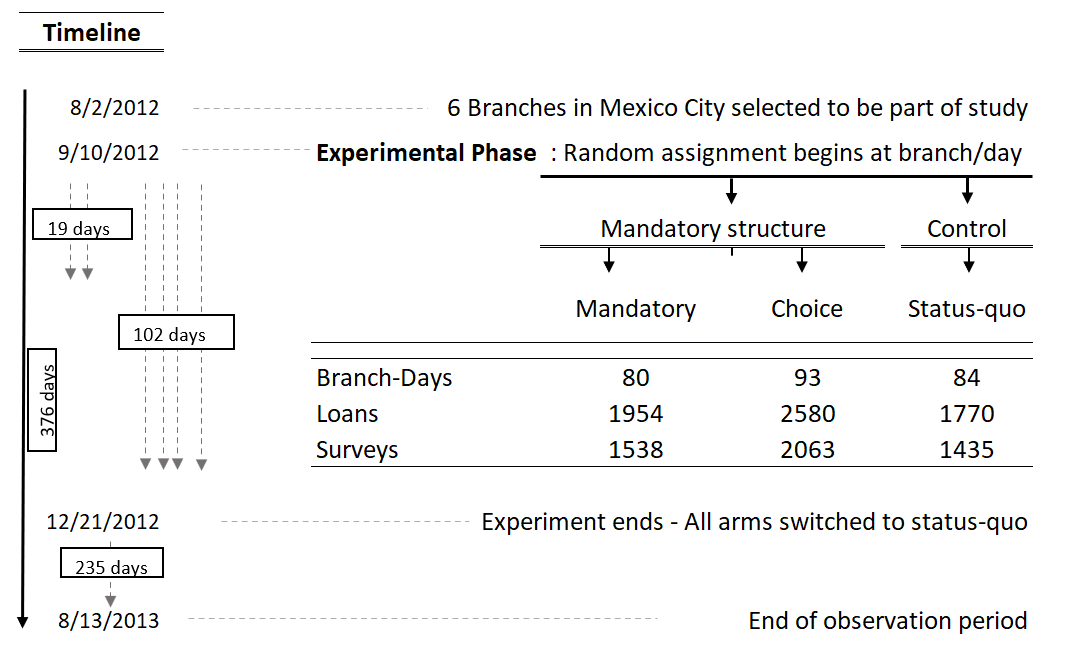
\includegraphics[width=0.9\textwidth]{Figuras/consort.png}
  \end{center}
     \label{exp_description}
%\textit{Do file: }  \texttt{consort.do}
\end{figure}


%\hfill \newline
%\noindent \textbf{Randomization.}  
\paragraph*{Randomization} We implemented the experiment in six branches of Lender $P$ beginning on September 9, 2012. The branches were selected by Lender $P$ to be dispersed across Mexico City and have varying sizes. In four of them the experiment ran for 102 days, and in 2 of them we ran it for a shorter time to economize on data collection costs once we realized we would not be constrained by sample size. %Thus we eliminated {the smallest} ones. 
Branches are more than 5 km apart from each other, and there is no substitution among them; none of the borrowers appear in more than one of our branches.

Branch personnel did not know which treatment would be assigned to each day and were blind to the objective of the intervention. They were told that there were 3 different ``types of contract-days'', that the system chose randomly for any given date, and that it could happen for instance that two or more consecutive dates had the same contract. They were also told that this way of operating was in place in several of Lender P's branches (they did not know which ones), and that it would be in place for several months. Randomizing at the day level limits the problem of contamination arising from clients realizing that other clients get different contracts than theirs. It also limits potential manipulation by appraisers, who in the presence of individual-level randomization could potentially pick their preferred customer from the line or tell them to wait until their desired contract shows up on the screen. Intra-branch day correlation on the probability of default (ICC) is small, at {0.05}, so we lose little power vis-a-vis individual-level randomization.


Some clients pawned more than one time during the duration of the experiment, with 14\% pawning 2 times and 8\% more than 2 times. To have a clean comparison we consider only the first pawn conducted during the experimental window. Moreover, 30\% of first pawns involve more than 1 loan, as 2 or more pieces of gold were submitted. We treat each of them as separate loans. In the appendix we show that our results are robust to this analysis choice. 

%\hfill \newline
%\noindent \textbf{Timeline.} 
\paragraph*{Timeline} Figure \ref{exp_description} shows the experimental timeline along with the length of time for which we observe payments. For loans made in the first week of the experiment, we observe up to 338 subsequent days of loan information; for loans made in the last week we observe up to 235 days. Figure \ref{exp_description} also illustrates the number branch-days per arm, the number of loans, and the number of surveys. %Not every contract has a survey for several reasons, we have survey information for \hl{XXX\%} of them. There were two reasons: \hl{XXX}.

%\hfill \newline
%\noindent \textbf{Explanation.} 
\paragraph*{Explaining the Contracts}
We made sure clients understood the contract terms.  First, we had full-time enumerators explaining contract terms to clients. The explanation took about 3-5 minutes and continued until the client said she understood the contract terms. Enumerators then asked clients to explain the contract back to them before correcting any misunderstandings. Second, the appraiser gave clients the ``Contract Terms Summary'' and read it out loud to them before after their piece had been appraised but before they signed the contract. %The sheet clearly indicates that this contract is a monthly payment one (numeral 1), that there is a penalty of 2\% for paying late (numeral 2), and the 3 payment dates (numeral 3). 
%Finally, the bottom of the Figure \ref{PaperSlip} shows the paper slip we used for the promise arms. The clients had to put their name on a slip of paper where they stated they promised to pay monthly.
We are confident the overwhelming majority of clients understood the contracts and that those in the choice arm made informed choices.
%\footnote{That we can systematically predict demand based on consumer characteristics and measured beliefs suggest that take up is not random.}


\subsection{Data}

%\hfill \newline
%\noindent \textbf{Administrative data.} 
\paragraph*{Administrative Data}
The study exploits two types of data: administrative data from the lender, and a short survey that we implemented. The administrative data contains a unique identifier for each client, an identifier for the piece she is pawning, and the transactions relating to that piece. These transactions include the value of the item as assessed by the appraiser, the amount of money loaned (70\% of the item's value), the date of the pawn transaction, and the type of contract for that pawn: structured payments or status quo. Within the period of the loan, we followed each transaction related to that piece in the administrative data: when payments were made and for what amounts, whether there was default (i.e.\ the client lost her pawn), and whether any late-payment fees were imposed. After the experimental loan, we are able to track subsequent behavior and to see whether that borrower took a subsequent loan.  We have this information for all the pawns that occurred in the experiment's 6 branches between August 2, 2012 and August 13, 2013. This includes all the pawns that took place during our experiment along with those that originated one month before and eight months after our experiment. Figure \ref{exp_description} shows the design and timing of the experiment, along with the sample sizes in each arm. The experiment comprises 6,304 pawns while our administrative data covers a total of 26,180 pawns.

%\hfill \newline
%\noindent \textbf{Survey data.} 
\paragraph*{Survey Data} An additional team of enumerators was stationed at the entrance of each branch; they asked clients to complete a 5-minute survey before going to the teller window to appraise their piece and \textit{before} they learned which contracts would be available on that day. The survey allows us to measure loan takeup since we know whether people entered the branch, completed the survey, and then, after learning the contract terms, decided not to pawn. As we will see, this is extremely infrequent; only about 3\% of borrowers did that. This is not very surprising, borrowers come determined to borrow, many of them to solve an emergency, and are not very sensitive to contract terms (that may explain why they accept high interest rates and over-collateralization in the first place). The survey was intentionally brief. It measured demographics, proxies for income/wealth, education, present-biased preferences, experience pawning, if family or friends commonly asked for money, how time-consuming and costly it was to come to the branch, the subjective probability of recovering the piece that they intended to pawn, the subjective value of their piece in money terms (how much money they would sell it for), among others. 
%We surveyed 7,210 clients. 
%, and our survey response rate was 78\% among clients who took loans. %\footnote{We also surveyed clients before and after the experiment, so our survey covers a larger sample that we are not using in this paper.}. 
%Is it important to say that we do \textit{not} use the survey for our main results. We only use the survey in Section \ref{Paternalism} of the paper.
The reported surveys are at the pawn level. One same borrower can have multiple surveys, one for each pawn, resulting in over 6,000 surveys.  

\subsection{Stylized facts}

%\hfill \newline
%\noindent \textbf{Borrowers.} 

\textcolor{red}{Given the scarcity of evidence about pawn loans in economics,  documenting stylized facts is a useful contribution. This section provides some important ones.}

\paragraph*{Borrowers.} Borrowers are not inexperienced: 87\% of clients in our survey report they have pawned before. %These clients have little or no access to other types of loans and they value the convenience of pawn borrowing.
However they are economically vulnerable:  20\% of them could not pay either water, electricity \& gas or rent in the past 6 months. In terms of triggers and uses of the loan, 89\% said they are pawning because of an emergency, and only 12\% stated it was to be used in a ``non-urgent expense''.  When asked why they are pawning this piece, 5\% responded ``lost a family member'', ``a medical emergency'' (11\%), or ``an urgent expense'' (72\%). Only 32\% of borrowers have completed college, 73\% are women, with an average age of 43 years.

%\hfill \newline
%\noindent \textbf{Many borrowers lose their pawn.} 
\paragraph*{Many borrowers lose their pawn.}
Our context is also one with high borrower default: 44\% of clients lose their pawn in a time span of 230 days from the date of pawning. One potential explanation for high default is that clients are really just knowingly selling their gold piece through a pawn contract on which they intend to default. This appears unlikely for several reasons: clients can easily sell the gold and obtain a higher amount of instant cash at gold-buying stores located close to almost all our pawnshop branches;
%(see Figure \ref{GoldBuyers}) 
the reported subjective value of the pawn is larger than the appraised value for 83\% of clients (this also means it is inefficient that they lose their pawns). The default rates for the experimental period and branches is similar to that observed for all branches in subsequent periods (see Figure \ref{external_validity}).  

\paragraph*{Gold buying shops.} Gold purchasing shops locate close to our Lender's branches. Branches have an average of 2.8 of these shops in the vicinity.  This fact is important given the high default rates which could indicate that borrowers are ex ante intending to ``sell'' their pawn.  Given that they are receiving 70\% of the value of the pawn next door to shops that would give them 100\% of this value, we think this is prima facie unlikely.
\todo[inline]{Referee asks: ``how do you define the vicinity and is it clear that the clients are aware of this?''}

\paragraph*{Paying without recovering.} Among those that lose their pawn, 29\% paid a positive amount towards its recovery. On average this subset of borrowers paid 34\% of the value of their loan (see Figure \ref{proxy_naive} in Appendix). This can only be rationalized if they expected to recover their pawn.

\paragraph*{Overconfidence.} 
Our baseline survey asked borrowers for their subjective probability of recovering the pawn. The average self-assessed recovery probability is 92\%. This contrasts sharply with the actual recovery rate for these same borrowers, 56\%. Overall 72\% of borrowers report a 100\% probability of repaying their loan.\footnote{\textcolor{red}{A recent paper by \cite{predatory2022} finds only the most inexperienced borrowers from a U.S. payday lender are overconfident, but their study examines priors about getting out of debt in the future rather than priors on repaying the current loan, as we do.}}    %Note that high default could be detrimental from the lender's point of view, since it may reduce the likelihood that the client becomes a return customer. 
%Lender P was in fact explicitly interested in partnering with us to investigate how to reduce loan default, customer satisfaction, and repeat borrowing.

    

\subsection{No differential selection or imbalance}
\label{sec:integrity}

%\hfill \newline
%\noindent \textbf{Attrition.} 

We were aware that the major threat to experimental validity in this study was selection into borrowing based on contract terms. We now show in three different was that there was \emph{no such selection}. First, among borrowers who entered the branch and completed the baseline survey (at which time they did not yet know their treatment status), 96.5\% end up pawning. This rate is not only high but is virtually identical across treatment arms. Second, the number of loans per day did not differ across experimental arms, showing that borrowers did not stop pawning when the structured arm or choice arm was active.  Third, borrower and loan characteristics are the same across arms, showing that there is no selection on observables.
%\footnote{Note that even if borrowers self-selected based on contract terms, the results would still reflect the overall impact of a treatment for the lender's portfolio. In our case, however, there was no such self-selection, so we can study the causal effects on borrowers.} 

An important implementation detail, mentioned above, is that appraisers were paid a flat wage, independent of how many contracts or which types of contracts borrowers signed. They therefore had no incentive to influence borrower choice. Consistent with this, adding or removing appraiser fixed effects leaves results unchanged. 
%We should also recall that the lender's management team initiated this research collaboration and genuinely wanted to rigorously measure the effects of a structured payment contract. Our lender is a non-profit and donates all profits to philanthropy. They had no profit incentive to sway the results either way and could not do it anyway as researchers designed, implemented, and analyzed the data without intervention from the lender.

Table \ref{attrition_table_final} uses administrative data to show there are no differences in the number of loans, borrowers, or amount borrowed across arms. Each row corresponds to a regression of the dependent variable on indicators for treatment assignment (status quo/control, structured repayment, choice). In the first row (``Take-up'') we use the sample of those individuals who answered the baseline survey (3710 subjects) and check which of them pawned based on the administrative data. The dependent variable indicates whether the person pawned. Because this survey was implemented at the entrance of the branch before they knew their treatment assignment, it is a good measure of take-up. The first result is that the overwhelming majority (96.5\%) take the loan. Second, the same fraction of borrowers take up the loan across treatment arms. This is strong evidence that borrowers did not select into treatment arms, which were announced between survey recruitment and contract completion. The remaining rows use only administrative data. For each branch day, we calculate the number of borrowers pawning, the number of pawns used, pawns per borrower, and the total amount borrowed and regress each of those on treatment arms. We again cannot reject that any of those measures of demand are the same across arms.  We also report medians to reduce the influence of outliers. \textcolor{red}{Overall, this strongly suggests that the treatments did not induce differential selection.}\footnote{Had we found differential selection, the cross-arm effects would still be relevant from the perspective of the lender, but would no longer represent intensive margin impacts on comparable groups of people.}

%This suggests clients were determined to borrow, and that frequent payments do not present an important hurdle in their desire do it; 87\% of surveyed borrowers have pawned before with Lender P.

\todo[inline]{The referee asks how the standard errors were computed in the Tables ``No Selection across arms'' and asks the same question for the ``tests of equality'' but I don't know what the latter refers to}

\begin{table}[H]
\caption{No selection across arms}
\label{attrition_table_final}
\begin{center}
\resizebox{0.65\textwidth}{!}{
\footnotesize{% Table generated by Excel2LaTeX from sheet 'Attrition'
\begin{tabular}{lcccr}
\toprule
      & Control & Structure & Choice & \multicolumn{1}{c}{p-value} \\
\midrule
\midrule
Loan take-up & 0.967 & 0.955 & 0.961 & 0.82 \\
      & (0.01) & (0.01) & (0.01) &  \\
\midrule
Number of borrowers & 20.8  & 22.2  & 25.4  & 0.17 \\
      & (3.29) & (3.9) & (4.89) &  \\
\rowcolor[rgb]{ .949,  .949,  .949} \multicolumn{1}{r}{median} & 19    & 20    & 21    & 0.5 \\
\midrule
Number of pawns/borrower & 1.4   & 1.4   & 1.4   & 0.43 \\
      & (0.08) & (0.04) & (0.05) &  \\
\rowcolor[rgb]{ .949,  .949,  .949} \multicolumn{1}{r}{median} & 1.4   & 1.3   & 1.3   & 0.6 \\
\midrule
Number of pawns  & 31    & 31.3  & 37.2  & 0.24 \\
      & (5.8) & (5.6) & (7.9) &  \\
\rowcolor[rgb]{ .949,  .949,  .949} \multicolumn{1}{r}{median} & 27    & 28    & 30    & 0.46 \\
\midrule
Amt borrowed/borrower & 2266.8 & 2094  & 2115.2 & 0.18 \\
      & (101.8) & (83.7) & (99.9) &  \\
\rowcolor[rgb]{ .949,  .949,  .949} \multicolumn{1}{r}{median} & 2154.3 & 2041  & 2047.5 & 0.65 \\
\midrule
Total borrowed & 47877 & 47813 & 54780 & 0.4 \\
      & (8005) & (9436) & (12587) &  \\
\rowcolor[rgb]{ .949,  .949,  .949} \multicolumn{1}{r}{median} & 37520 & 39420 & 40850 & 0.73 \\
\midrule
Obs   & 85    & 81    & 94    &  \\
\bottomrule
\bottomrule
\end{tabular}%
}
}
\end{center}
\scriptsize{Each row in this table 
 corresponds to a regression at the branch-day level of each dependent variable against the experimental arms indicators (control, mandatory structure , choice). The table reports the coefficients on each of these indicators, as well as the p-value of an F-test of the null hypothesis of equality of the three coefficients. We also report results using median regression. %Figure \ref{boxplot_attrition}, in the appendix shows a box-plot of the first two variables, showing the distribution across arms is balanced.
 }
%\textit{Do file: } \texttt{ss\_att.do}
\end{table}


%\paragraph*{Attrition} There are two main channels through which attrition could complicate the interpretation of our results. The first, and more serious, is the possibility that clients might change their pawning decisions in response to the treatment they encounter in a given branch on the day they enter the branch.  If this occurred it would introduce a self-selection dimension which would still reflect the overall impact of a treatment for the lender's portfolio but would no longer deliver \textit{ceteris paribus} effects of treatments on individual borrowers.  Narrative reports and the way the treatment was implemented make us believe that selection into treatment is unlikely.\footnote{Potential clients did not know that different days could have different contracts. If they asked, appraisers said that whatever was offered on that day was the only available contract for an undetermined length of time. Anecdotally, appraisers told us that they did not think refusals differed across arms, and our enumerators informed us that potential clients rarely left the branch without pawning. Lender P also never complained to us that our different treatments were hurting sales.} 

%If the treatments had induced demand-side selection, we would expect to see that the number of pawns successfully conducted differ in a systematic way across arms. That is, if potential borrowers disliked being forced into a structured payments contract, we would expect a lower number of pawns on branch days where only the structured payments contract is available compared to control days. Table \ref{attrition_table} shows that this is not the case. There is no difference at all between the Control and Forced structured payments arm in terms of the number of pawns per branch-day. %Although we cannot reject equality across the three arms (p-value=0.21), the Choice arm appears to have a somewhat larger number of borrowers than the Control and Forced arms.\footnote{p-value=0.23 and 0.12 respectively.} This seems to be due to sampling variability. The differences across arms are smaller when we look at medians, or when we look at the number of borrowers pawning (some borrowers pawn more than one piece). Figure \ref{boxplot_attrition} shows that full distribution of loans per day is very similar across treatment arms. The only noticeable difference is that the choice arm has a few more positive outliers.\footnote{If we winzorize at the 90th percentile, the mean number of branch-day pawns becomes identical across arms.}
%The bottom panel of Table \ref{attrition_table} shows balance in a more focused way, given that the surveys were conducted prior to the revelation of treatment status. We find that in no arm did more than three percent of individuals who responded to the survey go on to refuse loans. That is, the overwhelming marjority of potential borrowers did not leave the branch after learning which contract was on offer. Moreover, the extremely small fraction that did leave is balanced across arms.  Therefore it appears that the treatments have not induced any endogenous shifts in the composition of borrowers. 
%This is consistent with the findings of Table \ref{SS}.




% To test for this, we examine the number of loans given per branch-day, with specific attention to whether the Forced Commitment arm led to a lower number of borrowers per day. The first row of Table \ref{attrition_table} shows there is no difference between the Control and Forced Commitment arm in terms of the number of pawns per branch-day.\footnote{The Choice arm appears to have a somewhat larger number of borrowers than the Control arm (p-value=0.06), but we cannot reject equality with the Forced Commitment arm (p-value=0.41), or across all arms (p-value=0.16).}  The second row makes the same point in a more focused way, given that the surveys were conducted prior to the revelation of treatment status.  In no arm did more than three percent of individuals who responded to the survey go on to refuse loans, and neither these rates nor the rate of survey response are different across arms.  Therefore it appears that the treatments have not induced any endogenous shifts in the composition of borrowers.

% A less critical form of attrition is differential refusal to answer the survey questions.  The survey was conducted before treatment status was revealed, and we observe loan outcomes regardless of whether the survey was conducted.  Our core experimental estimates do not use the survey data as covariates, but the analysis in Section \ref{Paternalism} is restricted to the subset of borrowers who answered at least some survey questions. The bottom row of Table \ref{attrition_table} shows that the survey response rate is broadly similar across arms (about 78 percent). 

%We can also examine differences in the fraction of borrowers who do respond to the survey and then do not end up taking a loan subsequent to completing the survey, we find that the share is close to 100\% as is the fraction of those 97\% across arms (p-value=0.62).
%\footnote{We also tested if the number of pawns per day for the 6 branches that participated in the experiment was different 1 month before the experiment started or 1 month after the experiment ended, relative to the days the experiment was active. To this end we estimated the regression. We cluster the standard errors by branch.} $Pawns \: per \: day_{jt} = \alpha_j + \gamma f(t) + \beta_b \mathbbm{1}(t \in MB)_{t} +\beta_a \mathbbm{1}(t \in MA)_{t}$, where $\alpha_j$ are branch fixed effects, $f(t)$ is a third degree polynomial in time, $\beta_b$ measures a level effect in the number of pawns per branch a month before the experiment started, and $\beta_a$ a month after. We estimate no difference in the number of pawns, showing that people are not leaving the branch without pawning at larger rates during the experiment ($\beta_a=1.32$, $\beta_b=-0.65$, with p-values 0.11 and 0.83, respectively).  Table \ref{num_pawns_bal} shows the beta coefficients from these regressions, which are nowhere significant.}  Hence while survey response was not universal, there is no evidence that it was differential across arms.


%A more subtle form of sample selection could arise if the treatments induce borrowers to re-pawn in different ways, especially given that their treatment status on subsequent loan/days may not be the same as that initially assigned.  To address this issue our analysis uses only the first loan taken by each borrower during the experimental window.  

%\subsection{Connection to the literature}
%Our study connects with two strands of the literature on microfinance. But also to a nascent one that uses RCTs to study to what extent people self-sort to treatments that have larger beneficial treatment effects for them. On the microfinance literature the first paper we could find that used an RCT to evaluate the causal effect of frequent payments in loans is \cite{Pande}. In a group lending rosca context, they note that most contracts involved frequent repayments --even weekly in many instances-- even when this increases transaction costs. They note that clients could benefit from ``the fiscal discipline afforded by the more rigid payments''. Frequency could provide a commitment device for clients, could foster a payment habit, or could generate more trust from social interactions among the group of borrowers. All these potential benefits apply in our context, except those relating to social interactions, as we work with individualized loans.
   
%\subsection{More on implementation} %\label{implementation}

%\hfill \newline
%\noindent \textbf{Balance.} 
%\paragraph*{Balance} 

Table \ref{SS_final} presents summary statistics for the sample of actual borrowers across arms, showing that our randomization succeeded in achieving balance across the experimental arms. %Panel A uses administrative data for the universe of borrowers in each arm, and shows that loan balances and the days on the week on which individuals pawned are comparable across arms. The average loan size is \$2267 MXN (\$130 USD). Panel B of Table \ref{SS} reports summary statistics across arms from our survey data. 
%Among the 78\% of borrowers who completed our survey, 
73\% of surveyed borrrowers are women, the average age is 43 years, 66\% have completed at least a high school education, and 87\% have pawned before. Finally, borrowers' subjective probability of recovering their pawn is close to 92\%. The average subjective value they report for the items they pawn is 4084 MXN, much larger than the average appraised gold value of 3238 MXN. %While this could arise either from overconfidence in valuation or from undervaluation by the lender, in any case it is \textit{prima facie} evidence that loss of the pawn should be undesirable relative to the quantity of liquidity leveraged by the asset. 
Importantly, all borrower's characteristics are balanced across arms, again consistent with no differential selection across arms. Tables \ref{attrition_table_final} and Table \ref{SS_final}  tests are the standard experimental integrity analysis. Together they constitute strong evidence of no borrower selection across arms. This was reinforced by reports from our enumerators and appraisers that those who entered the branch were determined to borrow and that there were no complaints about what loan contracts were available. Importantly, this does \emph{not imply} that borrowers had no preference over alternative contracts. It simply means that the outside option of leaving the branch without a loan is unattractive.

\todo[inline]{The referee asks how the standard errors were computed in the Tables ``Borrower's characteristics are balanced'' and asks the same question for the ``tests of equality'' but I don't know what the latter refers to}

\begin{table}[H]
\caption{Borrower's characteristics are balanced}
\label{SS_final}
\begin{center}
\resizebox{0.65\textwidth}{!}{
\footnotesize{% Table generated by Excel2LaTeX from sheet 'SS'
\begin{tabular}{lcccccccc}
\toprule
      &       &       & \multicolumn{5}{c}{Treatment arms}    &  \\
\midrule
      &       &       &       & \multicolumn{2}{c}{No Choice } & \multicolumn{2}{c}{Choice} &  \\
\midrule
\midrule
      & Overall & Pre-experiment & Control & Fee   & Promise & Fee   & Promise & p-value \\
\midrule
      & \multicolumn{8}{c}{Panel A : Administrative Data} \\
\midrule
\midrule
Loan amount  & 2197  & 2239  & 2301  & 2147  & 2133  & 2181  & 2089  & 0.32 \\
      & (25)  & (39)  & (79)  & (72)  & (74)  & (65)  & (65)  &  \\
Monday & 0.18  & 0.16  & 0.18  & 0.16  & 0.17  & 0.19  & 0.21  & 0.96 \\
      & (0.02) & (0.03) & (0.05) & (0.05) & (0.06) & (0.06) & (0.05) &  \\
Number of branch-day pawns & 34    & 36    & 31    & 31    & 32    & 37    & 34    & 0.38 \\
      & (0.82) & (1.25) & (2.2) & (2.35) & (2.38) & (2.65) & (1.76) &  \\
\midrule
Number of branch-days & -     &       & 84    & 80    & 68    & 93    & 82    &  \\
Obs   & 21808 & 8366  & 2601  & 2484  & 2156  & 3435  & 2766  &  \\
\midrule
      & \multicolumn{8}{c}{Panel B : Survey Data (conditional on pawning)} \\
\midrule
\midrule
Woman & 0.73  &       & 0.76  & 0.72  & 0.73  & 0.72  & 0.74  & 0.41 \\
      & (0.01) &       & (0.02) & (0.02) & (0.02) & (0.02) & (0.01) &  \\
Age   & 43.31 &       & 43.16 & 43.17 & 42.96 & 43.96 & 43.06 & 0.79 \\
      & (0.28) &       & (0.57) & (0.79) & (0.65) & (0.61) & (0.52) &  \\
Subjective value & 3068  &       & 3151  & 2978  & 2985  & 3114  & 3079  & 0.41 \\
      & (39)  &       & (69)  & (91)  & (76)  & (85)  & (100) &  \\
Has pawn before & 0.9   &       & 0.89  & 0.9   & 0.89  & 0.91  & 0.89  & 0.68 \\
      & (0)   &       & (0.01) & (0.01) & (0.01) & (0.01) & (0.01) &  \\
Subj. pr. of recovery & 93.14 &       & 92.74 & 92.16 & 93.6  & 93.67 & 93.3  & 0.46 \\
      & (0)   &       & (0.55) & (0.86) & (0.6) & (0.47) & (0.6) &  \\
+High-school & 0.66  &       & 0.66  & 0.67  & 0.65  & 0.67  & 0.64  & 0.74 \\
      & (0.01) &       & (0.02) & (0.02) & (0.02) & (0.02) & (0.02) &  \\
Survey response rate & 0.78  &       & 0.77  & 0.75  & 0.8   & 0.77  & 0.79  & 0.5 \\
      & (0.01) &       & (0.02) & (0.03) & (0.02) & (0.02) & (0.02) &  \\
\midrule
Obs   & 10431 &       & 2000  & 1855  & 1732  & 2652  & 2192  &  \\
\midrule
\midrule
      & \multicolumn{8}{c}{Panel C : Survey Data (unconditional)} \\
\midrule
\midrule
Woman & 0.74  & 0.75  & 0.76  & 0.72  & 0.73  & 0.72  & 0.74  & 0.32 \\
      & (0.01) & (0.01) & (0.02) & (0.02) & (0.02) & (0.02) & (0.01) &  \\
Age   & 43.24 & 43.06 & 43.2  & 43.21 & 43.01 & 44.07 & 43.07 & 0.79 \\
      & (0.21) & (0.32) & (0.56) & (0.77) & (0.66) & (0.61) & (0.51) &  \\
Subjective value & 3112  & 3192  & 3145  & 2985  & 3010  & 3111  & 3082  & 0.41 \\
      & (36)  & (75)  & (68)  & (88)  & (76)  & (84)  & (99)  &  \\
Has pawn before & 0.89  & 0.88  & 0.89  & 0.9   & 0.89  & 0.91  & 0.89  & 0.56 \\
      & (0.01) & (0.01) & (0.01) & (0.01) & (0.01) & (0.01) & (0.01) &  \\
Subj. pr. of recovery & 92.64 & 91.84 & 92.73 & 92.19 & 93.66 & 93.71 & 93.34 & 0 \\
      & (0.2) & (0.31) & (0.54) & (0.84) & (0.59) & (0.46) & (0.59) &  \\
+High-school & 0.63  & 0.6   & 0.66  & 0.67  & 0.65  & 0.66  & 0.64  & 0.01 \\
      & (0.01) & (0.01) & (0.02) & (0.02) & (0.02) & (0.02) & (0.02) &  \\
\% ended up pawning &       &       & 0.98  & 0.97  & 0.99  & 0.98  & 0.99  & 0.25 \\
\midrule
Obs   & 17546 & 6919  & 2035  & 1907  & 1757  & 2710  & 2218  &  \\
\bottomrule
\bottomrule
\end{tabular}%
}
}
\end{center}
\scriptsize {The table uses survey data to show balance across arms. Survey data is not used for the main results of the paper. It is only used in Section \ref{why_paternalism}. Each row in this table corresponds to a regression, where the level of observation is a borrower that pawned which was surveyed.  The dependent variables are displayed in the first column. Each dependent variable is regressed against the experimental arms indicators (control, mandatory structure, choice). The table reports the coefficients on each of these indicators, as well as the p-value an F-test of the null hypothesis of equality of the three coefficients. ``Subjective value'' of the pawn refers to how much would the client be willing to sell the pawn for in pesos, ``Trouble paying bills'' is an indicator for the borrower reporting having problems paying electricity, water and services in the last 6-months, present bias is constructed as in \cite{Ashraf}; ``Makes buget'' as an indicator for whether the household make expenses budget for the month ahead of time. The subjective probability of recovery was elicited a la Manski (from 0 to 100 what is the probability that you will recoup your pawn); pawned before is a dummy=1 if the client declares to have pawned before (although not necessarily with Lender $P$); age is age of the borrower in years, +High-school is a dummy that indicates if the client has completed high school. 
}
%\textit{Do file: } \texttt{ss\_balance.do}
\end{table}


%\subsection*{Potential Outcomes and Exclusion}
%\label{sec:potentialOutcomes}
%\todo[inline]{This is a subsection that no longer exists but we need to go through and remove any cross-references to it.}

\section{The ``Mandates vs.\ Choice'' Design}
\label{sec:randchoice}

%\todo[inline]{The first paragraph of this section will need to be changed a bit to reflect its new location in the document. Since it's now a standalone section, I named it after our experimental design.}

We now develop more formally the assumptions that are required to translate the three-armed experiment of control, choice, and mandates into a structure that permits the point indentification of the Treatment on the Treated and the Treatment on the Untreated.  
%This section shows that, under an additional mild exclusion restriction assumption, our three-armed experimental design point-identifies a range of additional treatment effects of interest. 
%Foremost among them is the effect of treatment on the \textit{untreated}--those who would not demand structured repayment contracts--which is needed to assess the benefits mandating a contractual feature. 
We begin by providing a full definition of the potential outcomes in our empirical setting. Let $Z_i \in \{0, 1, 2\}$ denote the treatment arm to which to participant $i$ was assigned: $Z_i = 0$ denotes the mandatory no-structure arm, $Z_i = 1$ denotes the mandatory structured arm, and $Z_i = 2$ denotes the choice arm. 
Now let $D_i$ be the treatment that participant $i$ actually \emph{received}, where $D_i = 0$ denotes no-structure and $D_i = 1$ denotes structure. 
We assume perfect compliance in the $Z_i = 0$ and $Z_i = 1$ arms. %\footnote{For more discussion on this point, see Section \ref{sec:integrity} above.}
It is only in the $Z_i = 2$ arm that participants are free to choose between alternative contracts. 
Let $C_i \in \{0, 1 \}$ denote a participant's ``choice type.'' If $C_i = 1$ then participant $i$ \emph{would choose structure}, given the option; if $C_i = 0$ she would not. 
As shorthand, we call borrowers with $C_i = 1$ ``choosers'' and those with $C_i = 0$ ``non-choosers.''
Whereas a participant's choice type $C_i$ is only observed if she is allocated to the choice arm ($Z_i = 2$), her treatment $D_i$ and experimental arm $Z_i$ are always observed. 
Given the design of our experiment, these quantities are related by
\begin{equation}
D_i = \mathbbm{1}(Z_i \neq 2) Z_i + \mathbbm{1}(Z_i = 2) C_i.
\label{eq:potentialTreatments}
\end{equation}

We maintain the stable unit treatment value assumption (SUTVA) throughout. 
This means that borrower $i$'s outcomes depend only on her \emph{own} values of $Z_i$ and $D_i$, not those of any other person in the experiment. 
Under this assumption, a fully general model for the potential outcomes in our experiment would take the form $Y_i(d, z)$ for $d\in \{0,1\}$ and $z \in \{0, 1, 2\}$, allowing participant $i$'s potential outcome to depend \emph{both} on the treatment she actually receives, $D_i$, and the experimental arm to which she is assigned, $Z_i$. 
This model is too general, however, to point identify meaningful causal effects. 
For this reason we impose a standard exclusion restriction, namely
\begin{equation}
Y_i(d,z) = Y_i(d) \equiv Y_{id},\quad z \in \{0, 1, 2\}, \quad d\in \{0, 1\}.
\label{eq:exclusion}
\end{equation}
Mathematically \eqref{eq:exclusion} has the same structure as the standard LATE exclusion restriction. 
Substantively, however, its interpretation is a bit more specific, given that there is no explicit reference to the ``chosen'' versus ``mandatory'' treatment distinction in the usual LATE setup.
In our context, \eqref{eq:exclusion} implies that being assigned a particular treatment has the same result as choosing it for yourself.\footnote{Strictly speaking the results that follow \emph{only} require $Y_i(0,2)=Y_{i0}$ and $Y_i(1,2) = Y_{i1}$. In words: being assigned a particular treatment has the same result as choosing it for yourself, provided that that you are assigned the same treatment that you would have chosen freely.}
If the mere fact of having been given a choice has a direct effect on outcomes this assumption fails. 
For example: someone who, given the choice, would voluntarily choose to undergo drug rehabilitation, might respond differently when coerced.
In our experiment, however \eqref{eq:exclusion} is plausible.\footnote{Closely related assumptions are common, if often tacit. \cite{chamberlain2011bayesian} explicitly assumes that choosing and being assigned a treatment have the same effect. A significant literature using compulsory schooling laws to estimate the returns to education tacitly assumes that schooling \emph{in general} has the same returns, regardless of whether it is mandated or chosen freely. Similarly, fertilizer yields are tacitly assumed to generate the same returns regardless of whether the fertilizer was chosen by farmers or provided by the government, as long as it is the same fertilizer.} 
Moreover, it has testable implications that we fail to reject: see \autoref{sec:testing_exclusion}. 
Under \eqref{eq:exclusion}, the observed outcome $Y_i$ is related to $(Y_{i0}, Y_{i1})$ by 
\begin{equation}
    Y_i = \mathbbm{1}(Z_i =0) Y_{i0} + \mathbbm{1}(Z_i = 1)  Y_{i1}  + \mathbbm{1}(Z_i = 2) \left[(1 - C_i) Y_{i0} + C_i Y_{i1} \right].
\label{eq:potentialOutcomes}
\end{equation}

Equation \ref{eq:potentialOutcomes} is the key to understanding the mandates versus choice design. 
Random assignment of $Z_i=0$ and $Z_i = 1$ identifies the marginal distributions of $Y_{i0}$ and $Y_{i1}$ for the population as a whole. 
Random assignment of $Z_i=2$ likewise point identifies the share of choosers ($C_i = 1$), the distribution of $Y_{i1}$ for choosers, and the distribution of $Y_{i0}$ for non-choosers ($C_i = 0$).
Because $Z_i$ is assigned independently of pre-treatment covariates $X_i$, we also identify the \emph{conditional} distributions of $Y_{i0}$ and $Y_{i1}$ given $X_i$. 
As a direct consequence, our design point identifies a number of interesting and economically-relevant causal quantities. 
First among these are the treatment on the untreated (TUT) and treatment on the treated (TOT) effects:  
\[
\text{TUT} \equiv \mathbbm{E}(Y_{i1} - Y_{i0} | C_i = 0), \quad
\text{TOT} \equiv \mathbbm{E}(Y_{i1} - Y_{i0} | C_i = 1).
\]
The TUT is the causal effect of structure on borrowers who would not voluntarily choose it; the TOT is the causal effect on borrowers who would choose structure.
If the TUT is positive, this means that borrowers who did not choose structure would have experienced better outcomes, \emph{on average}, if they had. 

Figure \ref{tot_tut_graph} provides graphical intuition for why our design identifies the TUT and TOT. 
Viewing $Z_i$ as an instrumental variable, the Mandates versus Choice design can be seen as a \emph{pair} of RCTs, each subject to one-sided non-compliance.
The first compares $Z_i = 1$ to $Z_i=2$ and identifies the TUT.
By a standard argument (see Appendix \ref{sec:proofs}), 
\begin{equation}
\frac{\mathbbm{E}(Y_i|Z_i=1) - \mathbbm{E}(Y_i|Z_i =2)}{\mathbbm{E}(D_i|Z_i=1)-\mathbbm{E}(D_i|Z_i=2)} = 
\frac{\mathbbm{E}(Y_i|Z_i=1) - \mathbbm{E}(Y_i|Z_i =2)}{1 - \mathbbm{E}(D_i|Z_i=2)} = \text{TUT}.
\label{eq:TUT}
\end{equation}
since everyone with $Z_i=1$ is treated.
Similarly, since no one with $Z_i = 0$ is treated, a comparison of $Z_i=0$ to $Z_i = 2$ identifies the TOT:
\begin{equation}
\frac{\mathbbm{E}(Y_i|Z_i=2) - \mathbbm{E}(Y_i|Z_i =0)}{\mathbbm{E}(D_i|Z_i=2)-\mathbbm{E}(D_i|Z_i=0)} = 
\frac{\mathbbm{E}(Y_i|Z_i=2) - \mathbbm{E}(Y_i|Z_i =0)}{\mathbbm{E}(D_i|Z_i=2)} = \text{TOT}.
\label{eq:TOT}
\end{equation}
Because our design identifies by the TUT and TOT, it allows us to calculate the average selection on gains (ASG), the difference between the TOT and TUT effects:
\[
\text{ASG} \equiv \mathbbm{E}[Y_{i1} - Y_{i0}|C_i = 1] - \mathbb{E}[Y_{i1} - Y_{i0} | C_i = 0] = \text{TOT} - \text{TUT}.
\]
In a canonical Roy model $\text{TOT} > \text{TUT}$ so the ASG would be \emph{positive}.
The Mandates versus Choice design allows us to test this implication directly.

\begin{figure}
\caption{Graphical Intuition for the Mandates vs.\ Choice Design.} 
    \begin{center}
        \centering
        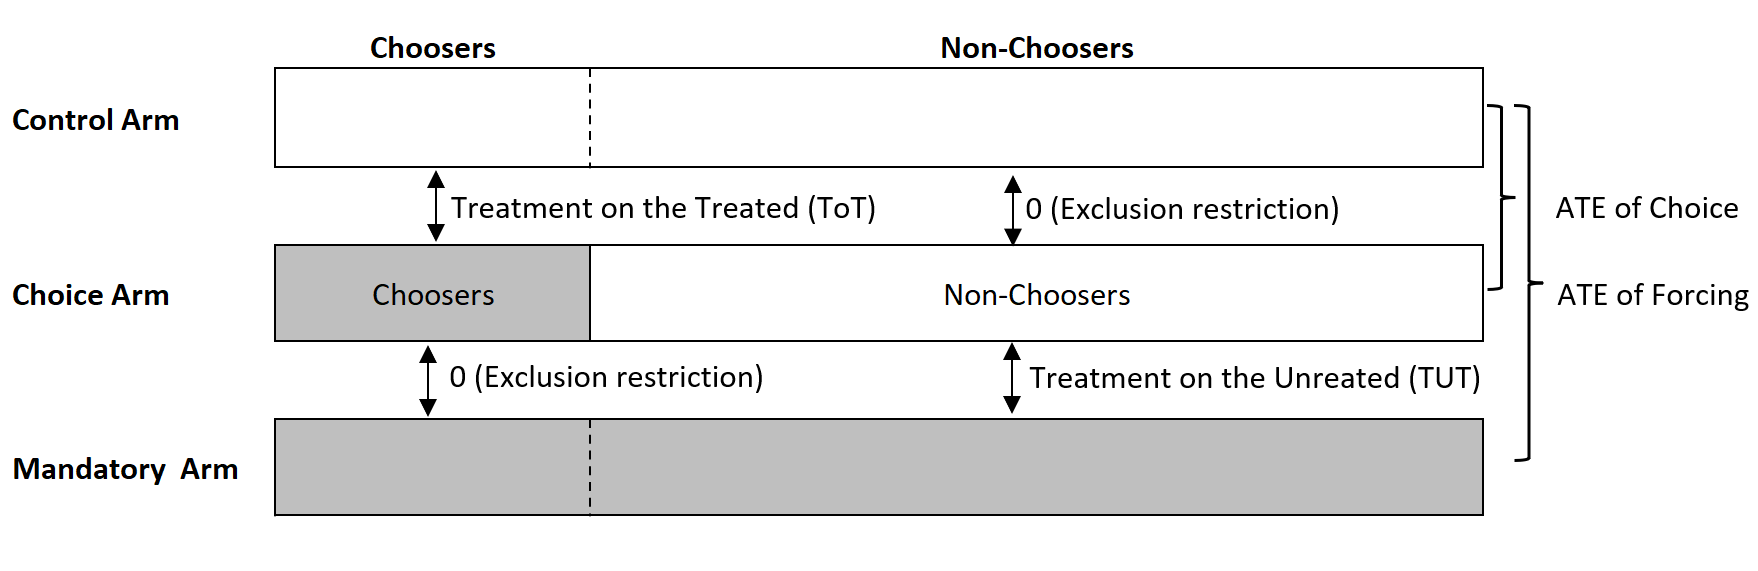
\includegraphics[width=1.0\textwidth]{Figuras/tot_tut_graph.png}
    \end{center}
 \scriptsize{
     %This figure illustrates why the controlled choice design identifies the TOT and TUT effects.
    Gray rectangles denote borrowers with a structured contract; white rectangles denote borrowers with a status quo contract. 
    A comparison of means across control and Structured arms identifies the ATE of Structure. 
    %In the choice arm, anyone with a commitment contract is a chooser; in the control and forcing arms, we do not know who is a chooser and who is not, but because borrowers are randomly assigned to experimental treatment arms, the share of choosers will be the same, on average (depicted using dashed vertical lines). 
    The difference of mean outcomes across the choice and control ``nets out'' the non-choosers, and hence equals the TOT multiplied by the share of choosers.
    %arms gives the intent-to-treat effect of offering choice. 
    %Under the exclusion restriction that moving non-choosers between the choice and forcing arms does not change their outcomes, this comparison ``nets out'' the non-choosers.
    %Hence, the ITT of offering choice equals the TOT multiplied by the share of choosers. 
    %Similarly, under the exclusion restriction that moving choosers between the choice and forcing arm does not affect their outcomes. 
    Similarly, the difference of means across the structured and choice arms ``nets out'' the choosers and equals the TUT multiplied by the share of non-choosers.
        The share of choosers, illustrated using dashed vertical lines, is equal on average across arms under random assignment.}
    \label{tot_tut_graph}
     %\textit{Do file: }  \texttt{tot\_tut\_graph.do}
\end{figure}   


A number of recent papers compare estimates of the TOT and TUT to better understand who selects into treatment and why, e.g.\ \cite{cornelissen2018benefits} and \cite{Walters}. 
This line of work relies, at least to some extent, upon structural modeling assumptions to extrapolate from the reduced-form quantities that are identified by the data alone to more interesting, and economically relevant, causal parameters.\footnote{While the marginal treatment effects (MTE) approach \citep{heckman2007econometric} can in principle be used to identify the TOT and TUT without parametric restrictions, doing so requires an instrumental variable $Z$ with sufficiently rich support that the probability of treatment take-up given $Z$ varies continuously between zero and one. In practice, instrumental variables are usually discrete and, even when continuous, typically have a more modest effect on take-up.} 
An alternative approach aims to avoid structural assumptions by calculating conditional local average treatment effects (LATE) given observed covariates $X$ and re-weighting them according to the distribution of covariates in some population of interest to yield, for example, an average treatment effect \citep{aronow2013beyond,angrist2013extrapolate}. 
%For example, one might re-weight using the distribution of $X$ in the population as a whole, rather than the sub-population of compliers, to extrapolate from LATE to ATE. 
But there is no free lunch: this ``LATE-and-reweight'' approach relies upon assumptions of its own, most crucially the assumption that there is \emph{no selection-on-gains} conditional on $X$, i.e.\ that the conditional LATE equals the conditional ATE. 
In contrast to both approaches, the Mandates vs.\ Choice design uses exogenous experimental variation to point identify the ATE, TOT, and TUT without ruling out unobserved selection-on-gains or relying on additional structural modeling assumptions.

In addition to the TUT, TOT and ASG, the Mandates vs.\ Choice design also identifies the average selection bias (ASB) and average selection on levels (ASL). In particular,
\begin{align}
\label{eq:ASB}
    \text{ASB} &\equiv \mathbbm{E}(Y_{i0}|C_i=1) - \mathbbm{E}(Y_{i0}|C_i = 0) = \frac{\mathbbm{E}(Y|Z=0) - \mathbbm{E}(Y|Z=2,D=0)}{\mathbbm{E}(D|Z=2)}\\
    \label{eq:ASL}
    \text{ASL} &\equiv \mathbbm{E}(Y_{i1}|C_i = 1) - \mathbbm{E}(Y_{i1}|C_i=0) = \frac{\mathbbm{E}(Y|Z=2,D=1) - \mathbbm{E}(Y|Z=1)}{1 - \mathbbm{E}(D|Z=2)}
\end{align}
as shown in \autoref{sec:proofs}.
The ASB tells us whether borrowers who voluntarily choose structure are those who are worse off, on average, under the status quo.
Similarly, the ASL tells us whether borrowers who voluntarily choose structure are those who are better off, on average, under the structured contract.
Equations \eqref{eq:TOT}--\eqref{eq:ASL} are useful for understanding why our experimental design identifies the TOT, TUT, ASG, ASB, and ASL but they are less convenient for estimation and inference. 
\autoref{sec:estimation_inference} explains how to compute each of these quantities from a small  number of just-identified, linear instrumental variables regressions, along with appropriate cluster-robust standard errors.
These estimators and standard errors are implemented in our companion STATA package. %\textcolor{red}{Add a link to this package along with the documentation.}


\section{Results} \label{Experiment}

%\todo[inline]{This section may need a new title: now it includes both ATE and TUT/TOT results.}


\subsection{Simple Experimental Results}

We begin our presentation of results with a standard estimation of experimental assignment to the Mandatory structured payments and the Choice arms, relative to the Control arm. As we explain below, only about 11\% of those in the choice arm chose the monthly payment option (Figure \ref{determinants_choose} shows coefficient plots for the characteristics that determine choosing structured payments in the Choice arm).

%\subsection{Average Treatment Effects}

%\hfill \newline
%\noindent \textbf{Specification.} 
\paragraph*{Specification} Table \ref{main_impact_table} presents estimates and standard errors from a standard pooled experimental regression 
\begin{equation} \label{basic_reg}
    y_{ij} = \alpha + \beta^M T_{i}^M + \beta^C T_{i}^C + \gamma X_{ij} + \epsilon_{ij}
\end{equation}
where $i$ indexes the borrower, $j$ indexes branch, $T_{i}^M$ and $T_{i}^C$ are indicator variables for receiving the Mandatory or Choice arms, $X_{ij}$ are branch and day-of-week fixed effects. Standard errors are clustered at the branch-day level, the unit of treatment assignment\footnote{A minority of borrowers pawned on more than one day during the experiment: 14\% pawned on two distinct days, and 8\% on three or more days. To avoid contamination from earlier treatments to which these individuals were exposed, we restrict our sample to each borrower's \emph{first visit}. Note that a borrower may pawn multiple items her first visit. We include these as separate observations. Because our standard errors are clustered at the branch-day level, they automatically account for any dependence in error terms arising from multiple pawns by the same borrower on her first visit.}.
Given full compliance in the Mandatory arm, the coefficient $\beta^M$ is the ATE of mandatory structure while $\beta^C$ is the ITT of structure in the Choice arm on the outcome variable $y_{ij}$.
%\footnote{Note that $\beta^C$ can be viewed in two ways: as the ATE of \emph{offering clients a choice} between the status quo and commitment contract or as the intent-to-treat effect of the commitment contract \emph{itself}. Here we adopt the former interpretation; below we use the latter to consider the relevance of selection-on-gains.}
Our two primary outcome variables are financial cost in pesos and Annual Percentage Rate (APR), as defined in Section \ref{costs}. 


Results for these outcomes appear in columns (1) and (7) of Table \ref{main_impact_table}.
The remaining columns decompose the financial cost and APR outcomes into their components: interest payments (col 2), payment towards any fees incurred (col 3), payments toward the principal (col 4). Column 5 shows the value of lost pawn conditional on losing it.  In column 6 the dependent variable is a dummy indicating default.  Finally, column 7 rescales financial cost as a function of loan size to estimate causal effects on incurred APR.\footnote{As we explained above, loans can be extended for an additional 3 months by paying the interest owed and restarting the loan under the same treatment conditions. This means that some loans extend for more than 3 months. We consider the entire flow of cost for the duration of our sample.}  

\begin{table}
\caption{Effects on Financial Cost}
\label{main_impact_table}
\begin{center}
\resizebox{1.0\textwidth}{!}{
\footnotesize{% Table generated by Excel2LaTeX from sheet 'decomposition_main_te'
\begin{tabular}{lcccccccc}
\cmidrule{3-7}      & FC    & Interest pymnt & Fee pymnt & Principal pymnt & Lost pawn value & Default &       & APR \\
\cmidrule{2-2}\cmidrule{9-9}      &       & $\sum_t P^i_{it}$ & $\sum_t P^f_{it}$ & $\mathds{1}(\text{Def}_i)}\times\sum_t P^c_{it}$ & $\mathds{1}(\text{Def}_i)}\times \text{Val-Loan Dif}_i$ & $\mathds{1}(\text{Def}_i)$ &       &  \\
\midrule
      & (1)   & (2)   & (3)   & (4)   & (5)   & (6)   &       & (7) \\
\midrule
\midrule
Forced commitment & -202.8*** & -157.3*** & 32.1*** & -0.61 & -77.6** & -0.065*** &       & -0.11*** \\
      & (48.1) & (34.9) & (1.43) & (2.88) & (31.6) & (0.023) &       & (0.019) \\
Choice commitment & -39.6 & -24.9 & 1.34** & -1.00 & -16.0 & -0.024 &       & -0.0089 \\
      & (49.8) & (38.4) & (0.54) & (2.62) & (33.1) & (0.021) &       & (0.019) \\
      &       &       &       &       &       &       &       &  \\
\midrule
Observations & 6304  & 6304  & 6304  & 6304  & 6304  & 6304  &       & 6304 \\
R-squared & 0.013 & 0.022 & 0.151 & 0.003 & 0.007 & 0.013 &       & 0.031 \\
Control Mean & 941.3 & 545.9 & 0     & 5.32  & 395.4 & 0.44  &       & 0.57 \\
\bottomrule
\bottomrule
\end{tabular}%
}
}
\end{center}
\scriptsize{This table shows the treatment effects for our core pecuniary outcomes. Each column is a different regression for different outcomes on an indicator for the mandated and choice arms, following specification in equation \ref{basic_reg}. Columns (1) \& (7) analyze our core financial cost measures, while the rest of the columns decompose these into finer components.
A few borrowers take more than one loan on the first day they appear in an experimental branch. These are treated as different observations. Additional results, available upon request, show that our results are robust to different ways of handling multiple loans for each borrower. Each regression includes branch and day-of-week FE. Standard errors are clustered at the branch-day level. }
%Table \ref{multiple_loans} shows our results are similar when dealing with the multiplicity of loans per borrower. 

%\textit{Do file: } \texttt{decomposition\_main\_te.do}
\end{table}



%\hfill \newline
%\noindent \textbf{Results.} 
\paragraph*{Results} The results are stark. The mandatory structure arm yields large and significant decreases in the cost of loans to clients, as measured either by financial cost or APR. Despite causing an increase in fees, the Mandated arm leads to a decrease of 204 pesos in the costs of borrowing (out of a group mean of 942 in the status quo), equivalent to 22\% reduction as a fraction of mean cost. These cost savings arise from a 6.6 percentage point (pp) decrease in the probability of default (out of a baseline mean of 44pp,  implying cost savings of 79 pesos), and also from lower interest payments since, as we will document below, the commitment-style contract speeds up payments so the interest rate applies to a smaller principal. This translates into a large reduction in APR. A credit product that has an effective average APR of 57\% in the status quo arm (inclusive of default) is reduced to a cost of 46\% through the imposition of a more regularized payment structure. This is in stark contrast to \cite{Pande} for instance.  

In contrast, to the impressive effectiveness of the mandatory structure arm, the Choice arm fails to deliver significant changes in any measure, with the exception of an increase in fees, for which we are highly powered, since this outcome is zero for every control observation. Giving borrowers the choice of contract did not decrease financial cost, whereas forcing them into a structured payment contract dramatically reduced it. As we explore later in the paper, the null effect of the Choice arm arises because few borrowers demanded structure (consistent with \cite{Ashraf}, \cite{Gine}, \cite{Ted}, \cite{Royer}, \cite{Sprenger}), with 89\% choosing the less effective status-quo contract.





\begin{landscape}
%\subsection{Intermediate Outcomes}
  
\begin{table}[!h]
\caption{Effects on intermediate outcomes}
\label{mechanisms}
\begin{center}

\scriptsize{% Table generated by Excel2LaTeX from sheet 'mechanism'
\begin{tabular}{lccccccc}
\toprule
      & \% of payment in 1st visit & $\Pr($Recovery in 1st visit) & \% of payment & $\Pr($+ payment \& default) & \% of pay $|$ def  & $\Pr($Selling pawn) & $\Pr($Selling pawn $|$ def) \\
\midrule
\midrule
      & (1)   & (2)   & (3)   & (4)   & (5)   & (6)   & (7) \\
\midrule
\midrule
Forced commitment & 7.92*** & 0.079*** & 9.43*** & -0.070*** & -3.90*** & 0.0050 & 0.14*** \\
      & (2.78) & (0.026) & (2.62) & (0.015) & (1.26) & (0.021) & (0.034) \\
Choice commitment & -0.97 & -0.010 & 1.40  & -0.026* & -1.75* & 0.0035 & 0.049* \\
      & (2.20) & (0.022) & (2.36) & (0.013) & (1.00) & (0.019) & (0.029) \\
      &       &       &       &       &       &       &  \\
\midrule
Observations & 6304  & 6304  & 6304  & 6304  & 2488  & 6304  & 2488 \\
R-squared & 0.014 & 0.016 & 0.015 & 0.011 & 0.022 & 0.016 & 0.033 \\
Control Mean & 44.7  & 0.30  & 67.2  & 0.12  & 9.46  & 0.31  & 0.72 \\
\midrule
\midrule
      &       &       &       &       &       &       &  \\
\midrule
      & Days to 1st payment & \# of visits & \# of visits $|$ recovery & \# of visits $|$ def & Loan duration (days) & Loan duration $|$ recovery &  \\
\midrule
\midrule
      & (8)   & (9)   & (10)  & (11)  & (12)  & (13)  &  \\
\midrule
\midrule
Forced commitment & -13.8*** & -0.031 & -0.19*** & 0.062 & -27.9*** & -17.9*** &  \\
      & (1.61) & (0.049) & (0.049) & (0.053) & (4.35) & (3.88) &  \\
Choice commitment & -3.51** & 0.085 & -0.077* & 0.13** & -0.18 & -1.35 &  \\
      & (1.57) & (0.053) & (0.041) & (0.063) & (4.33) & (4.19) &  \\
      &       &       &       &       &       &       &  \\
\midrule
Observations & 4412  & 6304  & 2488  & 3031  & 6304  & 3031  &  \\
R-squared & 0.055 & 0.022 & 0.025 & 0.018 & 0.054 & 0.041 &  \\
Control Mean & 82.8  & 1.14  & 0.39  & 1.44  & 136.6 & 103.9 &  \\
\bottomrule
\bottomrule
\end{tabular}%
}

\end{center}
\footnotesize{This table explores treatment effects in ``intermediate variables''. Each column represents regression output for different dependent variables following equation (\ref{basic_reg}). Panel A focuses on variables related to the speed of payment. While Panel B focuses on variables related to default, and Panel C related to visits. 
% The outcome variables are as follows:  number of days elapsed between origination and first payment (col 1); percentage of the loan paid in the first payment (col 2); probability of recovery in the first visit (col 3); loan duration is the number of days the borrower took to payoff her loan for those that recover, the number of days until default for those that default, and the maximum number of days we observe them in the sample for those that have not recovered or defaulted (col 4); loan duration conditional on recovery; an indicator for paying a positive amount towards recovery but nonetheless losing the pawn (col 6); the percentage or the loan paid, conditional on defaulting --`wasted payments' (col 7). Column 8 uses the phrase `selling the pawn' for a dummy variable indicating the borrower did not pay any amount towards recovery and lost the pawn. Moreover, (col 9) shows that treatment effects are concentrated in the intensive margin as treatment does not affect the fraction of clients who pay a positive amount towards pawn recovery. The dependent variable in column 10 is the number of day-visits to the branch (measured by the existence of transactions that day associated with our particular pawn), while column 11 conditions on borrowers that lost the pawn.
Each regression includes branch and day-of-week FE. Standard errors are clustered at the branch-day level.}
%\textit{Do file: } \texttt{mechanisms.do}
\end{table}
\end{landscape}

\normalsize
%Really force it to normal size and linespread
\normalsize



%\hfill \newline
%\noindent \textbf{Intermediate outcomes.} 
\paragraph*{Payment speed} To shed light on the mechanisms behind the ATEs discussed above, Table \ref{mechanisms} shows how structure affects a number of intermediate outcomes. One can group the types of intermediate outcomes into two categories: measures of the speed of pawn recovery, and measures of the decision of when to default. While the first payment for borrowers in the status-quo contract occurs on average only on day 82 (on a 90 days contract), borrowers in the mandatory structure arm start paying 13.8 days earlier on average (col 1). Not only do they start paying earlier, the first payment is also 9.7\% larger (col 2), and a larger fraction (7.9\%)  actually pay in full and recover their pawn in the first payment, compared to 30\% in the status quo contract (col 3). The resolution of the loan (either by payment or default) is shortened by 27.9 days (col 4), and conditional on recovery (an endogenous control) by 17.9 days (col 5).

\paragraph*{Payment Bifurcation} A very undesirable outcome from the borrower's perspective is to pay towards the loan without paying in full, i.e.\ to default on the loan despite making some payments. In this case, borrowers lose both the collateral and any payments made toward recovery. One could be concerned that by encouraging them to pay monthly, more borrowers might end up in this dire scenario in the mandatory structure contract. Column 6 shows this is not the case. On the contrary, 7 percentage points fewer borrowers end up in this situation, compared to a status quo contract mean of 12 percent. Conditional on defaulting those assigned to the mandatory structure contract have paid 4.1\% less of their loan (col 7), and a 14 percent higher proportion of borrowers pay zero conditional on defaulting, an outcome analogous to
``selling their pawn'' (col 8). One interpretation of this bifurcation is that the mandatory structure contract forces borrowers to think earlier about whether they will indeed be able to eventually recover their pawn, and separates borrowers into those ``selling'' their pawn and those recovering it, reducing the share of undecided borrowers that end up paying interest and end up losing the pawn anyway. This mechanism may also help to explain why the mandatory structure contract does not increase the number of visits to the branch to pay (col 10): those recovering their pawn visit more, but those defaulting have 0.20 fewer visits (col 11). Finally, Column 9 shows that treatment effects are concentrated in the intensive margin as treatment does not affect the fraction of clients who pay a positive amount towards pawn recovery.



%\noindent \textbf{Other costs.} 
\paragraph*{Other Costs} Although the paper focuses on financial costs, we consider three additional costs here. First, we include the cost of visiting the branch to make a payment. This includes the self-reported transport cost (most use public transport), as well as the opportunity cost of time. To err on the conservative side, we subtract a whole day's minimum wage for the day of the visit. 
%instead of just the wage corresponding to a couple of hours. 
Second, we consider a rough proxy of the value of liquidity that borrowers lose by paying sooner. To do this we add the interest costs on to the payments in the mandatory structure arm and recompute treatment effects with these payments compounding daily (as if they had to borrow in order to make the more rapid payments). Third we consider the \emph{subjective} value of the pawn. All results presented thus far value the collateral as appraised by the lender, but the piece may be worth more to the borrower than its gold value. For many of them the pawned jewelry has sentimental value. This is reflected in the subjective valuation they reported in the survey, which is almost twice as large as the appraised gold value of the pawn on average. Our third extra cost considers this higher subjective value. Table \ref{table_robustness_fc} shows that our results are robust to all these changes. 

It is worth emphasizing that our results do not directly measure borrower welfare. 
Financial cost savings and welfare could diverge in a number of ways.
%We want to be very clear that we are not measuring borrower welfare, for several obvious reasons. 
For example, requiring monthly payments could cause an increase in borrowers' levels of stress, an effect that our measures do not take into account.
Moreover, given the short time frame of pawn loans, we do not explicitly account for discounting.
As shown in Section \ref{why_paternalism}, however, one would need to assume unreasonably high discount rates to cast doubt on our findings. 
Similarly, we cannot measure the financial cost of other loans that borrowers may potentially take out to make interim payments on their initial pawn loan. 
Given that the ``penalty'' from a missed interim payment is small--less than the transport cost to visit the branch--we consider it unlikely that borrowers will have taken out even more expensive loans to avoid the penalty.
%However, we think it is unlikely that borrowers ask for even more expensive loans to pay the monthly payment. The `punishment' from the monthly fee is small, less than the transport cost to go to the branch. It is likely better to incur the fee than go through the process of asking for an additional loan to avoid this fee.} 
Having said this, a large literature focuses on the cost of servicing loans. We follow in the steps of this literature. 



%\hfill \newline
%\noindent \textbf{Repeat Pawns.}
%Another way to push the analysis towards a consideration of borrower welfare is the conjecture that if clients exposed to the installment contract like it, they will be more likely to come back vis-a-vis those that got status quo contract.\footnote{\cite{Laibson2018} hypothesizes that consumers use ``experienced utility'' as a guide to make future purchases in this way.} This is indeed what we find in the data.  We consider this outcome in Table \ref{repeat_loans}. We can first ask whether the individual ever takes a loan after the initial study loan, an analysis which is simply experimental.


%\hfill \newline
%\noindent \textbf{Censoring of Loan Completion.}
\paragraph*{Censoring of Loan Completion}
The window of time during which we were able to observe borrower behavior was limited in each branch, meaning that there were loans that we do not see completed (particularly those pawns that were rolled over for one or two further 90-day spells).  Overall, 13\% of all experimental loans are censored, meaning that they neither default nor repay within the observation window.  In the prior analysis we handle this issue in a conservative way by using outcomes such as ``did not default'' which are well-defined even when we do not observe the completion of the loan, resulting in an estimate biased toward zero by the more rapid loan repayment observed in the Structured arm.  In the Online Appendix we consider this issue in more detail.  Most importantly, Table \ref{bounding_censoring} conducts a bounding exercise that examines how large the effects of this censoring could possibly be by making bracketing assumptions about repayment on censored loans in the treatment and control, respectively.  Comfortingly, Panel B of this table shows that even the most muted possible effect in the bounding exercise still recovers impacts of Structure on financial costs and APR that are negative and significant at the 99\% level.  Using a lasso-logit model to predict the outcome of censored loans, Panel E shows the APR impact of Structure increases from a 11 pp reduction (headline results) to a 17 pp reduction.  Hence there appears to be no scope for this censoring issue to overturn our results, and our core results (implicitly assuming censored loans are not defaulted) is almost certainly an under-estimate of the true impacts.

\todo[inline]{Regarding the next paragraph on lender profit, the referee asks: ``in the computation of profit you also assume independence between repeat and the amounds. Couldn't you simply model total financial costs as a function of the duration observed to extrapolate?''}

\paragraph{Lender profit} One of the questions we are interested in is whether lender profits decrease with structured payment. If that is the case, lenders will have little incentive to include this feature in their contracts. For a single loan, lenders get what borrowers lose in a zero-sum way so that a borrower's Financial Cost$_i$ for loan $i$ is the profit from that loan for the lender. Table \ref{main_impact_table} showed that borrowers pay less to lenders \emph{per loan} under the structured payments contract. However, in Table \ref{repeat_loans} in the appendix, we show that borrowers assigned to the mandatory structure arm are 6.7\% more likely than in the status quo arm to be repeat customers during our sample period. This brings some extra benefit to lenders that we take into account in a simple back-of-the-envelope calculation. From column 1 of Table \ref{main_impact_table}, $\mathbbm{E}\left[\text{Financial Cost}_i | \text{Contract=X}\right]$ for $X$= \{status quo, structure\} contracts are approximately \$942MXN and \$738MXN. From Table \ref{repeat_loans} we know $\Pr(\text{Repeat} | \text{Contract}=X)$ for $X$= \{status quo, structure\} are 32\% and 38.7\%, respectively. We can use these four numbers to calculate a discounted sum of profits for client $j$ comparing a scenario where only status quo loans are offered with a second scenario where only structured payment loans are offered.\footnote{We do this for simplicity. Otherwise, we would have to assume something about how borrowers switch dynamically across types loans, and this is something we do not observe in the data.}  
Assuming independence across repawning events within a given contract type gives  
\[
\text{Profit}_{j,X}  = \sum_{t=0}^T\delta^t\mathbbm{E}\left[\text{Financial Cost}_j | \text{Contract}=X\right]\times\Pr(\text{Repeat} | \text{Contract}=X)^t
\] 
where $\delta$ is the discount rate.  We find that for every  $\delta$ $\in$ [0,1]    and for every $T$ the status quo results in higher profit for the lender. That is, the extra repeat probability for the structured payment contract is not enough to compensate for the loss in each of those loans.\footnote{An alternative calculation is as follows: $\text{Profit}_{j,X} = \{\text{Financial Cost}_j | \text{Contract}=X\}\{1+n\times\Pr(\text{Repeat}_j)\}$ where $n$ is are exogenously arising need to borrower, which are lead to repeat pawning. In this case, the status quo contract dominates (profit-wise) the structured payment contract for all $n$.} Figure \ref{profit_mandatory_control} in the appendix shows the examples for different values of $\delta, T$.


%\section*{Choice and Heterogeneous Treatment Effects}
%\label{Choice}

%\todo[inline]{This title refers to the old version: we will need to remove cross-references to it}

%\todo[inline]{The next paragraph needs to be revised given how we're restructuring things. Should the Chernozhukov stuff appear alongside all the other heterogeneous treatment effects material? Also, this paragraph used to \emph{precede} our introduction of the potential outcomes. Now that it follows it, it seems like a bit much.}


%If the effect of structure were homogeneous, this would be enough to conclude that the 89\% who did not choose it would have been financially better-off if they had.
%In a world of heterogeneous treatment effects, however, low demand for commitment could still be consistent with borrowers adhering to a standard model of rational choice. 
%The borrowers who did not choose structure could simply be those who don't need it. 
%Indeed, we find strong evidence that the effect of mandatory structure varies substantially across individuals in our experiment: we test and reject
%Appendix \ref{append:chernozhukov} tests and rejects 
%the null hypothesis of homogeneous treatment effects using the methodology of \cite{chernozhukov2018generic} (details available upon request).
%So the question remains: can we explain the 89\% of borrowers not choosing commitment as being those that don't benefit financially from it?  
%In this section, importantly, we show that structure would lower average financial costs even for the subset of borrowers who choose \emph{not} to commit voluntarily.


%\todo[inline]{We need a transition here}

\subsection{Estimating Treatment Effects by Compliance}

The results from above show that commitment \emph{works}: clients who were assigned to the mandatory structure arm experienced substantially lower financial costs on average.  In spite of this, given the opportunity, only 11\% of borrowers chose this structure freely. The central question driving the relative benefits of mandatory versus voluntary compliance concerns the relationship between treatment effects and the choice to adopt the structured payments, or selection on gains.  We now proceed to exploit the exclusion restrictions presented above to separately estimate treatment effects for the choosers and non-choosers of the structured payment contract.  Table \ref{tot_tut} calculates the causal quantities described above---TOT, TUT, ASG, ASB, and ASL---for our experimental data, along with robust standard errors for each.\footnote{To simplify the exposition in this and all sections that follow, we re-define all outcome variables so that \emph{beneficial} treatment effects are \emph{positive}. Using this convention, a positive treatment effect of structure on financial cost, for example, reflects the average cost \emph{savings} caused by structure.} 
For purposes of comparison, the table also presents the ATE results from Section \ref{Experiment} above (row 1),\footnote{Coefficients are not exactly the same since Table 4 includes branch and day-of-week FE.} along with the corresponding average potential outcomes $\mathbbm{E}[Y_0]$ and $\mathbbm{E}[Y_1]$ (rows 4--5).
The columns of the table correspond to different outcome variables defined above.
We are now in a position to report one of the important results in the paper. For all four outcome definitions, the TUT effect is positive, statistically and economically significant, and comparable in magnitude to the ATE.
In other words: the structured payments contract is on average \emph{beneficial} to the people who \emph{would not choose it}, and these benefits are large. That is, mandating structured payment contracts would decrease the financial cost. Borrowers are leaving money in the table by not choosing it. 

Some comments are in order. First, this result holds on average. Some non-choosers could lose from a mandate. Section \ref{sec:RF} assesses personalized targeting strategies. Second, financial cost is not welfare, and further work with more comprehensive measures (stress, consumption, performance in other loans) needs to be done. We provide proof of concept that at least financial cost may not be minimized by free choice and provide a method to rigorously compare take-up mandates against consumer choice. Third, given that providing such contracts may not be in the lender's interest, borrowers may not even be presented with this choice.

Table \ref{tot_tut} also estimates the TOT effect. Due to the low take-up rate in the choice arm, TOT effects are imprecisely estimated. Only one of them, \%(1-Default) from column (3), is statistically significant. 
This carries over into our estimates of the average selection on gains. Our point estimates are \emph{negative} for all but the (1 - Default) outcome, but none is statistically distinguishable from zero.  
%Although we cannot quite reject the null hypothesis that the TUT and TOT effects are equal--our power is limited because of the low take-up rate of commitment in the choice arm--the pattern of coefficients is consistent with some degree of selection-on-gains.
%Commitment is more beneficial to people who are willing to choose it than it is to people who are not.
For the (1 - Default) outcome, we have sufficient precision to conclude that the average selection bias (ASB) is large and negative.
This means that borrowers who choose structure would have faced a higher probability of default under the status quo contract than borrowers who do not choose structure.%\footnote{We may not want to read too much into TOT vs TUT comparisons as they are imprecise. But taken at face value, the result that TOT$>$TUT for default, while the opposite is true for financial cost, suggests that, while voluntary commitment has a slightly stronger effect on allowing borrowers to avoid default, forcing \textit{reduces} payments in a strong enough manner as to overcome the default-benefits of choice.}  


Overall, Table \ref{tot_tut} suggests that structure works but that \emph{not enough} people choose it: the structured contract saves money on average even to those who would \emph{not} choose it voluntarily. We believe this result is new in the household finance literature. It also illustrates how the ``Mandates vs.\ Choice'' design can be used more generally to understand the relationship between choice and treatment effect heterogeneity, in particular the causal effect among non-choosers.\footnote{For instance, in the debate on financial commitment take-up, some papers argue that this effect is low (\cite{Ashraf}, \cite{Gine}, \cite{Ted}, \cite{Royer} while others argue it is high (\cite{Kremer}, \cite{Casaburi}, \cite{Alcohol}, \cite{AprajitP&P}, \cite{Pascaline}), but none estimates the benefits for non-takers. In a different domain, doctors claim that medical treatment abandonment is too high in a broad range of diseases \citep{non_adherence}, without knowing the treatment benefits for those that abandon.}

\begin{table}[H]
\caption{Five Treatment Effects Estimates: TOT, TUT, ASG, ASB, ASL}
\label{tot_tut}
\begin{center}
\footnotesize{% Table generated by Excel2LaTeX from sheet 'tot_tut'
\begin{tabular}{lcccc}
\toprule
      & APR \% benefit & FC benefit & \% Recovery & \% (1-Default) \\
\midrule
      & (1)   & (2)   & (3)   & (4) \\
\midrule
\midrule
ATE   & 34.6*** & 386.1*** & 13.3*** & 7.57*** \\
      & (8.25) & (117.6) & (2.56) & (2.50) \\
ToT   & 119.5* & 624.2 & 15.4  & 37.3* \\
      & (67.7) & (1086.7) & (20.4) & (21.5) \\
TuT   & 24.5*** & 357.7*** & 13.1*** & 4.02* \\
      & (8.26) & (107.9) & (2.71) & (2.40) \\
E[Y1] & -182.5*** & -1847.7*** & 43.3*** & -43.4*** \\
      & (5.92) & (69.4) & (1.95) & (1.69) \\
E[Y0] & -147.9*** & -1461.6*** & 56.6*** & -35.8*** \\
      & (5.75) & (95.0) & (1.65) & (1.84) \\
\midrule
ToT-TuT & 95.1  & 266.5 & 2.37  & 33.2 \\
      & (71.0) & (1133.8) & (21.6) & (22.5) \\
      &       &       &       &  \\
\midrule
Observations & 6304  & 6304  & 6304  & 6304 \\
Control Mean & -182.5 & -1847.7 & 43.3  & -43.4 \\
H_0 : ATE-TuT=0 & 0.18  & 0.81  & 0.91  & 0.14 \\
H_0 : ATE-ToT=0 & 0.18  & 0.81  & 0.91  & 0.14 \\
H_0 : ToT-TuT=0 & 0.18  & 0.81  & 0.91  & 0.14 \\
H_0 : ToT-TuT$\geq$ 0 & 0.091 & 0.41  & 0.46  & 0.070 \\
\bottomrule
\bottomrule
\end{tabular}%
}
\end{center}
\scriptsize{This table presents results computed using the derivations from Section \ref{sec:randchoice}. The APR and financial cost outcomes have been multiplied by $-1$ so that a positive causal effect \emph{benefits} the borrower in each of the four columns. The bottom panel presents p-values for a number of null hypothesis tests of treatment effect heterogeneity. }
%\textit{Do file: } \texttt{tot\_tut.do}
\end{table}




%Below we explore possible explanations for this result.
%and the ``right people'' choose to commit: those who are most likely to benefit from it and those whose outcomes are most adverse under the status quo. 



%Given that the ITT results for the Choice arm imply an insignificant worsening of outcomes relative to the control, our estimates of the Treatment on the Treated in the first row of the bottom panel show negative results that are larger in absolute magnitude (multiplied by ~9, the inverse of the compliance rate) and similarly insignificant.  The Treatment on the Untreated (TuT), conversely, is strongly positive across the board, and indicates a significant improvement for all outcomes (here ITTs are effectively multiplied by 1.12, the inverse of the non-compliance rate).  Most novel is the ability to form a test of the difference between the ToT and the TuT, which is conducted in the bottom rows of the table.  We provide four different ways of estimating p-values for this comparison; the standard clustered estimates motivated by the experimental design, normal and percentile bootstraps, and randomization inference.  The differences between treatment effects for compliers and non-compliers are of borderline significance in some of the unadjusted specifications, but are not significant once adjusted.\footnote{It is worth noting that the statistical power of these estimands is driven by the compliance rate; given our low overall compliance we are better powered to measure the TuT than the ToT, and the power for the difference between the two would be highest with a compliance rate of 50\%.}   Because of the large standard errors on the ToT coming from the low compliance rate in the Choice arm we are unable to state with statistical confidence that the TuT is higher than the ToT, but the TuT is strongly positive while the ToT is weakly negative, and so in both relative and absolute terms the choices being made are `wrong' relative to the potential outcomes.




%\todo[inline]{Possibly add some discussion here of Craig's idea: using the controlled choice design to study ``targeting''}

%A unique feature of our design is the randomized assignment to treatment (forced commitment), control (forced no-commitment), and choice of treatment. 

%This structure allows us to observe the average value of both the treated and untreated potential outcomes, as well as the selection into treatment that would occur under choice.  A starting point for how to exploit this structure is to apply the logic usually used to estimate the Treatment on the Treated (ToT) to also recover the Treatment on the Untreated (TUT).  This approach assumes nothing about the decision to choose (other than random sampling generating counterfactual compliance rates that would have been the same in every arm), but imposes three exclusion restriction-style assumptions typical of Local Average Treatment Effect (LATE) analysis.  Namely, a) the typical assumption that an individual not choosing the treatment has the same potential outcome as one not offered it, then b) the mirror image assumption for the Forcing arm that an individual forced to take Commitment has the same potential outcome as an individual freely choosing it, and c) no spillovers from chooser to non-choosers in the choice arm.\footnote{\hl{For robustness we also try a Manski-type monotone IV approach with similar results.}}


%More formally, let $Z_i$ be the observed, randomly assigned experimental allocation, where $Z_i=0$ denotes the control arm, $Z_i=1$ denotes the Forced arm, and $Z_i=2$ is the Choice arm.  Let $C_i$ be the choice type; $C_i=0$ when individual $i$ does not choose commitment and $C_i=1$ when chooses commitment, observed in the Choice arm and latent in the other two arms.  A fraction $p$ of individuals chooses the treatment in the Choice arm.  Finally, $D_i = Z_i\times \mathds{1}(Z_i\neq 2) + C_i\times \mathds{1}(Z_i=2)$ is the observed treatment indicator, and $Y(d,z)$ is the potential outcome function for $d=0,1$, and $z=0,1,2$.


%To test the difference between gains for choosers versus gains from non-choosers we need to identify $\mathbb{E}[Y_1-Y_0\;|\;C=1]$ (the Treatment on the Treated), and $\mathbb{E}[Y_1-Y_0\;|\;C=0]$ (the Treatment on the Untreated).   The observed outcome in the Choice arm is the weighted average of the treated and untreated outcomes; $p \times\mathbb{E}[Y_1\;|\;C=1] + (1-p)\times\mathbb{E}[Y_0\;|\;C=0]$.  Given assumptions a) and c) above we can recover the ToT from the difference between the Choice and Control arms as is standard, and then symmetrically we can invoke b) and c) to recover the TUT from the difference between the Forced and Choice arms as follows:

%\begin{align*}
%ToT \equiv \mathbb{E}[Y_1 - Y_0 \;\mid\; C=1]  &=   \frac{\mathbb{E}[Y \;\mid\; Z=2] - \mathbb{E}[Y \;\mid\; Z=0]}{p} \\
%TuT \equiv \mathbb{E}[Y_1 - Y_0 \;\mid \;C=0]  &=  \frac{\mathbb{E}[Y \;\mid\; Z=1] - \mathbb{E}[Y \;\mid\; Z=2]}{(1-p)} 
%\end{align*}


%This estimate of the ToT is the standard one that would result from instrumenting for compliance with the offering of treatment as in \cite{angrist1996identification}.  The TuT is the analogous estimator, which could be recovered in a regression pooling the forced and choice arms and instrumenting for \textit{not} complying with being assigned to the choice arm (for a more formal development, see the appendix).  The advantage of representing the estimands via division of the relevant ITT by the compliance (non-compliance) rate is that it allows us to estimate all the necessary terms from the single pooled regression Equation \ref{basic_reg}, from which the significance levels for the ToT, the TuT, and the difference between them can all be estimated as single-equation F-tests:


%\[ToT = \frac{\beta^C}{p}; \qquad\quad TuT = \frac{(\beta^F - \beta^C)}{(1-p)}; \qquad\quad (ToT-TuT) = \frac{\beta^C}{p}- \frac{(\beta^F - \beta^C)}{(1-p)}. \]


%\hfill \newline
%\noindent \textbf{TOT and TUT results.} 


%\section*{The Case for Mandating Structure} 
%\label{Paternalism}
%\todo[inline]{This section has been replaced, but we'll need to go through and remove / update the cross-references to it.}

\section{Behavioral Drivers}
\todo[inline]{This is a working title; we may well want to change it}
\label{why_paternalism}

A behavioral literature has highlighted voluntary commitment as an attractive way of allowing the ``right'' people to self-select. % A discussion of compulsory commitment is necessarily paternalistic, and by its nature focuses on impacts among those who would not have selected commitment voluntarily. 
%Viewed through the lens of rational choice theory, it is unsurprising that we estimate $\text{TOT}>\text{TUT}$. 
The argument for compulsory treatment, centers on the surprising result that $\text{TUT}>0$. We now investigate four potential explanations for the positive $\text{TUT}$: the need to learn, time discounting, present bias, and overconfidence.
   

%\hfill \newline
%\noindent \textbf{Learning.}  

Our experiment introduced a new contract into an environment that had not previously featured structured repayment; perhaps clients required experience to understand its benefits. Are clients who experienced the commitment contract more likely to choose structure subsequently than those assigned to the status-quo contract? %We have already shown above that those who experienced the Forcing contract were more likely to borrow again.  We now ask whether the subset who were assigned to the Choice arm when they returned were more likely to choose commitment.  
Appendix Table \ref{learning_table} compares borrower assigned to the mandatory versus status quo arms on an initial pawn who then return to take a subsequent loan at a branch offering choice.  %\footnote{Table \ref{learning_table} presents information about participants' \emph{immediate subsequent} pawning behavior.  For borrowers who returned to pawn again more than once, this analysis considers only their first repeat pawn.}
This analysis shows \textit{no difference} in choosing structure for the 22\% of borrowers in these two initial arms who returned to pawn again and were offered choice.   %The implication is that while those who have experienced commitment feel more positively towards the pawn contract, the experience does not lead them to conclude that they need commitment on the subsequent loan.  
While these exercises cannot completely exclude the possibility that learning would play a role with more exposure, they provide no indication that the lack of voluntary compliance is simply a matter of inexperience with structure in the short run. Note also that there will be no learning if lenders don't provide a structured payment contract in the first place.


%Column (1) considers the 228 clients who returned only a second time to pawn again at a day/branch that was randomly assigned to the choice arm. Each of the two rows in this column presents a difference of mean commitment take-up rates, and associated standard error. The first row compares those who were \emph{initially} assigned to forced commitment against those where were assigned to control; the second row compares those who were initially assigned to the choice commitment arm to those who were assigned to the other two arms. In each case, there is no statistically discernible difference in the rates of commitment take-up. Granted, this is a selected sample because the decision to pawn again is potentially endogenous to the initial treatment allocation. For this reason, Column (2) considers the full sample of 4441 borrowers by re-defining the outcome variable to be an indicator for returning to pawn again at a branch/day when commitment was offered \emph{and} choosing commitment. This composite outcome variable is not subject to the sample selection problem (although it is directly driven by the decision to repeat borrow). The comparison in the two rows remains the same: forced commitment versus control in row one and choice commitment versus forced arms in row two. Again, there is no statistically discernible difference in commitment take-up rates in either row. While these exercises cannot completely exclude the possibility that learning plays a role, they provide no indication that the lack of voluntary compliance is simply a matter of inexperience with commitment.


%\hfill \newline
%\noindent \textbf{Time discounting.}  

Can high borrower time discount rates explain low demand for structured payments? %Highly impatient individuals might rationally choose the \emph{status quo} contract, despite the benefits that commitment yields returns, 
After all, monthly payments are front-loaded while pawn recovery is back-loaded, even if by only a few weeks.  
%those returns are realized at contract ending hile the cost of monthly payments are incurred  Our estimated decrease in the financial cost of credit from above ignores discounting, but commitment involves incurring up-front costs (early payment) in return for delayed benefits (a higher probability of recovering one's pawn). 
Figure \ref{fc_discount_rates} calculates TUT effects for different borrower discount rates given the actual timing of repayment and pawn recovery. The solid line gives the TUT effect adjusted for a specified annual discount rate, while the shaded regions give the associated 95\% \& 90\% confidence interval.
We see that non-choosers continue to experience significant decreases in the net present value of financial costs up to annual discount rates of 1,000\%, an extremely high level of impatience.\footnote{In a similar exercise for subprime borrowers in the US, \cite{Levin} argue that even discount rates smaller than these would be too large to be reasonable and can be safely discarded as explanations.} As such, discounting is unlikely to explain why those who benefit, on average, from structure fail to choose it. % when offered. 


%\hfill \newline
%\noindent \textbf{Present bias.} 
If the benefits of structure among non-choosers cannot be explained by standard models of rational choice, the canonical behavioral story would center on time inconsistency.  While commitment is useful to anyone with hyperbolic time preferences, only those who are sophisticated---i.e.\ aware that they are hyperbolic discounters---will demand it.  A large share of ``na\"ive'' hyperbolics in the population--borrowers who are unaware that they are hyperbolic discounters--could therefore drive a large and positive $\text{TUT}$.  Our baseline survey included standard questions about discount rates between tomorrow and a month in the future versus discount rates between three and four months in the future.
This allows us to classify borrowers who display more impatience over immediate delays as present biased. This measure of financial hyperbolicity is widely used in survey research, although it is not without problems.\footnote{\textcolor{red}{We also asked a simple self-reported question about temptation, and obtain similar answers with this alternate measure.} Recent empirical work has shown the superiority of more elaborate measures such as ``convex time budgets'' \citep{andreoni2015measuring} while questioning the interpretation of measures of hyperbolicity that are not based on consumption \citep{andreoni2012estimating, cohen2020measuring}, suggesting that real effort tasks provide a better measure \citep{augenblick2015working}.  Given that we had only a few minutes to interview real pawnshop clients prior to a commercial transaction, our simple measure was a necessary compromise.}   

If we could perfectly measure present bias and sophistication, we could divide the sample into three groups: sophisticated hyperbolics (who chose structure), time-consistent non-choosers (for whom structure will not be effective), and na\"{i}ve hyperbolic non-choosers (who will benefit from structure even if not chosen by them). %If present bias fully explains the low take-up rate of voluntary commitment, we should find that the TUT for present-biased borrowers  is positive while the TUT for all other borrowers is not.
If present bias explains the low take-up rate of voluntary commitment, we should find that the TUT for present-biased borrowers is larger than for other borrowers. This is because among the group of non-takers, a comparison of present-biased borrowers against everyone else is a comparison of na\"{i}ve hyperbolics against time-consistent non-choosers. The left panel of Figure \ref{tut_beh_partition} in the Appendix carries out a feasible version of this exercise using our survey measure of present bias.
%The overall TUT estimate along with a 95\% confidence interval is given in blue.\footnote{For all borrowers who answered our present-bias survey questions.}
%The corresponding TUT estimate and confidence interval for present-biased borrowers identified with the survey question is given in green; results for all other borrowers are shown in red.
%The overall TUT is a weighted average of the impact in these two sub-groups.  The TUT among the present biased is insignificant and less than half the size of the strongly significant TUT among those who are \textit{not} present biased. Therefore, taking our survey measure of hyperbolicity at face value. 
We find no indication that present-bias explains our positive estimated TUT.\footnote{Similarly, we find that experience pawning does not predict TUT.}



%\hfill \newline
%\noindent \textbf{Sure confidence.} 

Finally, motivated by the high subjective probabilities of recovery we found in the baseline survey, and by the fact that a large fraction of borrowers pay towards recovery and then lose the pawn and these payments, we explore overconfidence in recovery as a potential explanation of low demand for structured payments. After all, recall that while 72\% of survey respondents believe they have a 100\% chance of recovering their pawn, in reality only 43\% will go on to do so.  
Borrowers who are certain to recover their pawn perceive no benefit of committing to repay under the threat of fees and, therefore, no benefit of choosing the structured payment contract.
%if individuals who \emph{believe} that they are certain to repay, choose (rationally given their incorrect beliefs) to forgo the costs associated with commitment that are designed to induce repayment. 
To explore this, as in the preceding paragraph, we compare the overall TUT estimate to estimates computed for two sub-groups, defined by a binary variable that we call ``sure-confidence''. This measure equals one for any individual who says at the time of borrowing that they have a 100\% probability of recovering their pawn, and zero otherwise.
%The right panel of Figure \ref{tut_beh_partition} presents the results for this exercise.
%The overall TUT estimate for all borrowers who answered our sure-confidence survey questions is given in blue, along with a 95\% confidence interval.
%The corresponding TUT estimate and confidence interval for sure-confident borrowers is given in green; results for all other borrowers are shown in red.
In contrast to our results for present bias, we find that sure-confidence \textit{is} a strong predictor of TUT. Figure \ref{tut_beh_partition} shows that the TUT is almost entirely confined to the sure confident individuals, while those that say they have some chance of defaulting have TUT close to zero. It seems that the effectiveness of paternalism in our experiment may be driven by \emph{overconfident} borrowers who, heedless of the risk of default, fail to choose structure despite benefiting substantially when it is mandated.\footnote{In Figure \ref{determinants_sure} we plot the coefficient estimates from a regression that predicts sure confidence with a battery of individual-level characteristics.  Older males are more likely to be sure-confident, as are those with more education.  Taken at face value, the sure-confident also report less financial stress, less trouble paying bills, and to be more frequently relied upon financially by family members.  Viewed through a behavioral lens, however, it is also possible that the type of person who is over-confident in their ability to repay a loan also exaggerate their degree of economic security in their response to survey questions. In any case, it appears that sure confidence may be difficult to predict with easily-observed and objective demographic criteria, a point to which we return below.}


\section{Understanding Treatment Effect Heterogeneity} \label{sec:RF}
\todo[inline]{This is a working title; we may want to change it}

\subsection{Bounding the Distribution of Individual Treatment Effects}
\label{sec:bounds}
\todo[inline]{Now that this section appears after we defined all of the potential outcomes, we don't need to define them: we just need to reference the section where they were defined.}

Calculating the number of individuals who benefit from mandatory structure requires the distribution of individual treatment effects.
While this distribution cannot be point identified, it can be bounded.
Let $(Y_{i0}, Y_{i1})$ be $i$'s potential outcomes under the control and mandatory structure conditions and define $\Delta_i \equiv Y_{i0} - Y_{i1}$.
Let $(F_0, F_1, F_\Delta)$ be the marginal distributions of $(Y_{i0}, Y_{i1}, \Delta)$ and define 
\[
\underline{F}(\delta) \equiv \max \left\{0, \sup_y F_1(y) - F_0(y - \delta)  \right\}, \quad
\overline{F}(\delta) \equiv 1 + \min \left\{0, \inf_y F_1(y) - F_0(y-\delta) \right\}.
\]
Since $F_0$ and $F_1$ are point identified under random assignment, so are $\underline{F}$ and $\overline{F}$, and the pointwise sharp bounds for $F_\Delta$ are $\underline{F}(\delta) \leq F_\Delta(\delta) \leq \overline{F}(\delta)$ \citep{fan2010sharp}.
Figure \ref{fan_park_bounds} plots these bounds for the APR outcome in our experiment.  
To bound the share of borrowers who benefit from mandatory structure, we merely substitute $\delta=0$ into the preceding, since $\mathbb{P}(\Delta_i > 0) = 1 - F_\Delta(0)$.
Our point estimates of $\underline{F}(0)$ and $\overline{F}(0)$ are 0.03 and 0.77 respectively, with 95\% confidence intervals of [0.025, 0.050] and [0.75, 0.80]. Since we are interested in $\mathbbm{P}(\Delta_i >0) = 1 - F_\Delta(0)$, it follows that \textit{at least 23\%}, and at most 97\%, of individuals borrowers benefit from mandatory structure.\footnote{Confidence intervals are constructed using the asymptotic distribution of $(\underline{F}, \overline{F})$. See \cite{fan2010sharp}.} 
\todo[inline]{Need to add explanation of how we incorporated covariates in carrying out this exercise: see editor's comment.}
That is, even under the most conservative possible assumptions, we find evidence of depressed demand: more than 23\% would benefit from structured repayment but only 11\% demand it. 
These bounds are wide because they concern the distribution of \emph{individual treatment effects} and make no assumptions beyond our experimental randomization. 
By adding assumptions it is possible to say more. 
For example, under rank invariance\footnote{i.e.\ if $i$'s rank in the distribution of $Y_0$ equals her rank in the distribution of $Y_1$} the distribution of treatment effects is point identified and given by $F_\Delta(\delta) = \int_0^1 \mathbbm{1}\{ F_1^{-1}(u) - F_0^{-1}(u)\leq \delta\}\,\mathrm{d}u$, where $F_1^{-1}$ and $F_0^{-1}$ are the quantile functions of $Y_1$ and $Y_0$.\footnote{Figure \ref{te_rankinvariance} in Appendix \ref{bounds_FOSD} plots our estimates of $F_\Delta$ under rank invariance.} Because in our data, $Y_1$ first-order stochastically dominates $Y_0$ for financial benefit ($F^{-1}_1(u) - F^{-1}_0(u) >0$), we conclude that all borrowers would benefit ($\Delta_i > 0$). 


%%%%%%%%%%%%%%%%%%%%%%%%%%%%%%%%%%%%%%%%%%%%%%%%%%%%%%%%%%%%%%%%%%
% Original Version before trimming for ECTA
%%%%%%%%%%%%%%%%%%%%%%%%%%%%%%%%%%%%%%%%%%%%%%%%%%%%%%%%%%%%%%%%%%
%If we knew the distribution of individual treatment effects, it would be easy assess how many individuals would win and lose under a policy of universal forced commitment, along with the magnitude of any individual harm. 
%Because we can never simultaneously observe the same borrower in both the control and forced commitment arms, however, the distribution of individual treatment effects cannot be point identified.
%It can, however, be bounded.
%We begin our exploration of heterogeneous treatment effects by computing assumption-free bounds on the share of individuals who benefit from forced commitment. 
%
%Let $Y_{i0}$ be borrower $i$'s potential outcome under the control condition, $Y_{i1}$ be her potential outcome under forced commitment, and $\Delta_i \equiv Y_{i0} - Y_{i1}$.
%Because it randomly assigns borrowers to the control and forced arms, our experimental design point identifies the marginal distributions of $Y_{i0}$ and $Y_{i1}$, call them $F_0$ and $F_1$.
%Now, define the functions $\underline{F}$ and $\overline{F}$ as follows:
%\[
%\underline{F}(\delta) \equiv \max \left\{0, \sup_y F_1(y) - F_0(y - \delta)  \right\}, \quad
%\overline{F}(\delta) \equiv 1 + \min \left\{0, \inf_y F_1(y) - F_0(y-\delta) \right\}.
%\]
%Since $F_0$ and $F_1$ are point identified, so are $\underline{F}$ and $\overline{F}$.
%\cite{fan2010sharp} show that the sharp (best possible) pointwise bounds for $F_\Delta$ are given by $\underline{F}(\delta) \leq F_\Delta(\delta) \leq \overline{F}(\delta)$.
%These bounds are simple to compute, and can be surprisingly informative. 
%Here we use them to bound the fraction of borrowers who benefit from forced commitment. 
%Given the way that we have defined our outcome variables, this is the share of borrowers whose treatment effect is positive, i.e.\ $\mathbb{P}(\Delta_i > 0) = 1 - F_\Delta(0)$. 
%To construct the sharp bounds for this quantity, we simply substitute $\delta = 0$ into the preceding equations and estimate $F_0$ and $F_1$ using their empirical analogues constructed from the forced commitment and forced no-commitment arms of the experiment.
%
%Figure \ref{fan_park_bounds} plots the sharp bounds for $F_{\Delta}$ based on the APR outcome. Our point estimates of $\underline{F}(0)$ and $\overline{F}(0)$  are 0.03 and 0.77 respectively, with associated 95\% confidence intervals of [0.025, 0.050] and [0.75, 0.80]. Since we are interested in $\mathbbm{P}(\Delta_i >0) = 1 - F_\Delta(0)$, this means that \textit{at least 23\%} of individual borrowers benefit from commitment (and at most 97\%).\footnote{Confidence intervals are constructed using the asymptotic distribution for the bounds. See \cite{fan2010sharp} for details.}
%
%The bounds we have just described are constructed by considering all possible joint distributions of $Y_0$ and $Y_1$ that are compatible with the observed marginal distributions $F_1$ and $F_0$. 
%With stronger assumptions, it is possible to say more.
%One such assumption is \emph{rank invariance}, which posits that a person's rank in the distribution of $Y_0$ equals her rank in the distribution of $Y_1$.
%While strong, this assumption or variants of it have appeared in a number of settings in the literature, e.g.\ \cite{chernozhukov2005iv}, so we consider it here for purposes of comparison.
%Under rank invariance, the distribution of treatment effects is point identified and given by 
%\[
%F_\Delta(\delta) = \int_0^1 \mathbbm{1}\{ F_1^{-1}(u) - F_0^{-1}(u)\leq \delta\}\,\mathrm{d}u 
%\]
%where $F_1^{-1}$ and $F_0^{-1}$ are the quantile functions of $Y_1$ and $Y_0$. Figure \ref{te_rankinvariance} in Appendix \ref{bounds_FOSD} plots our estimates of $F_\Delta$ under rank invariance.
%For the financial benefit outcome, $Y_1$ first-order stochastically dominates $Y_0$ in our experiment. Since this implies that $F^{-1}_1(u) - F^{-1}_0(u)$ is always positive, rank invariance yields an extremely stark conclusion: all borrowers have positive individual treatment effects of forced commitment. 
%For the APR outcome, the results under rank invariance are slightly less stark: we estimate that just under 90\% of borrowers have positive individual treatment effects. 
%%%%%%%%%%%%%%%%%%%%%%%%%%%%%%%%%%%%%%%%%%%%%%%%%%%%%%%%%%%%%%%%%%
% End of original version before trimming for ECTA
%%%%%%%%%%%%%%%%%%%%%%%%%%%%%%%%%%%%%%%%%%%%%%%%%%%%%%%%%%%%%%%%%%




%\noindent \textbf{Causal forests.} 
On average, the structured contract benefits both those who would choose it and those who would not.
In Section \ref{sec:bounds}, we briefly went \emph{beyond} average effects by presenting bounds on the distribution of individual treatment effects.
Because they made no assumptions beyond random assignment, these bounds were relatively wide.
%Adding the assumption of rank invariance yielded a distribution of treatment effects in approximately 90\% of borrowers had positive individual treatment effects for the APR outcome, implying that \emph{practically everyone} would benefit from treatment and hence that there would be hardly any no losers from paternalism. Rank invariance, however, is an extremely strong assumption.\footnote{For the financial cost outcome, rank invariance implies that all invididual treatment effects are positive.}
We then applied NAE assumptions to estimate average treatment effects for choosers and non-choosers. 

In this section, we again impose NAE exclusions, but this time conditional on observed covariates, not just on average. This enables us to use causal forests to estimate \textit{conditional} average treatment effects (CATE) as well as CTOT and CTUT effects. This stronger assumption allows us to say more about personalized treatment effects and, therefore, to assess different ways to target structured payments.  %This exercise provides more fine-grained information about treatment effect heterogeneity.
Among other things, it will potentially allow us to identify groups of borrowers who are on average \emph{harmed} by structure.
%Under the stronger assumption that our observed survey measures capture the main sources of treatment effect heterogeneity, this exercise will allow us to approximate individual-level counterfactuals, to consider whether particular borrowers made ``mistakes'' in their choice of contract. 
To estimate the conditional average treatment effects we use the ``generalized random forest'' methods of \cite{atheygrf} (see Appendix \ref{app:cate} for details).\footnote{The generalized random forest approach of \cite{atheygrf} produces conditional average effect estimators that are asymptotically normal.
Our inferences in this section are carried out by simulating from the normal limit distributions using the estimated standard errors. As covariates, we use 22 questions in our survey (what we call the \textit{wide} set of covariates in Appendix \ref{app:cate}. The survey questionnaire (with the highlighted questions being the ones for the wide set of covariates) can be found in \ref{baseline_survey} in the Appendix. \textcolor{teal}{ \cite{burke2022credit} use a generalized random forest algorithm to explore heterogeneity in the effects of credit builder loans on the credit score.}}
We implement these estimates using the covariates from our survey.

\vspace{.2in}
\begin{figure}[!h]
     \caption{Heterogeneous Treatment Effects.} 
     \label{heterogeneous_effects}    
    \begin{center}
     \begin{subfigure}{0.35\textwidth}
       \centering
      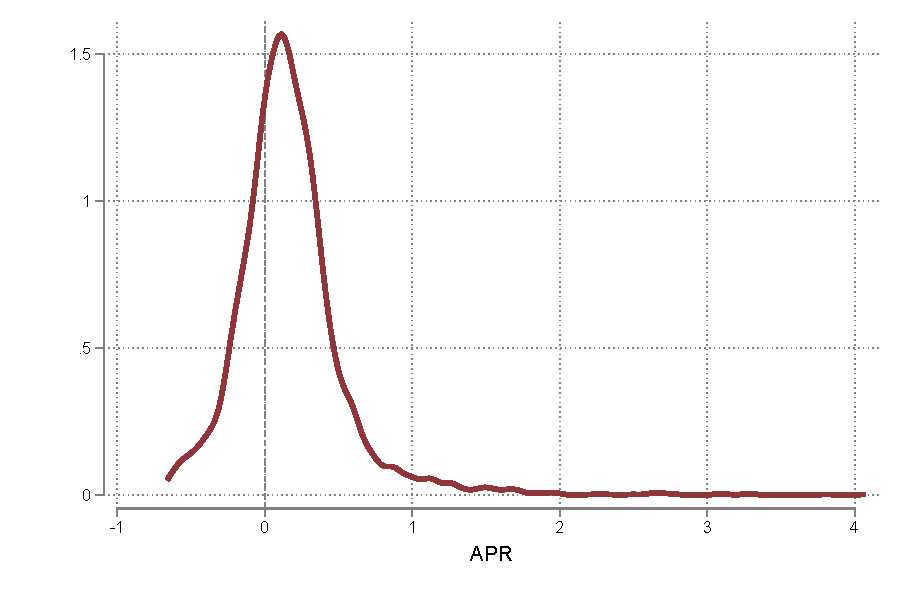
\includegraphics[width=\textwidth]{Figuras/he_dist_tau_hat_tot.pdf}
          \caption{Conditional TOT}
    \end{subfigure}
    \begin{subfigure}{0.35\textwidth}
       \centering
      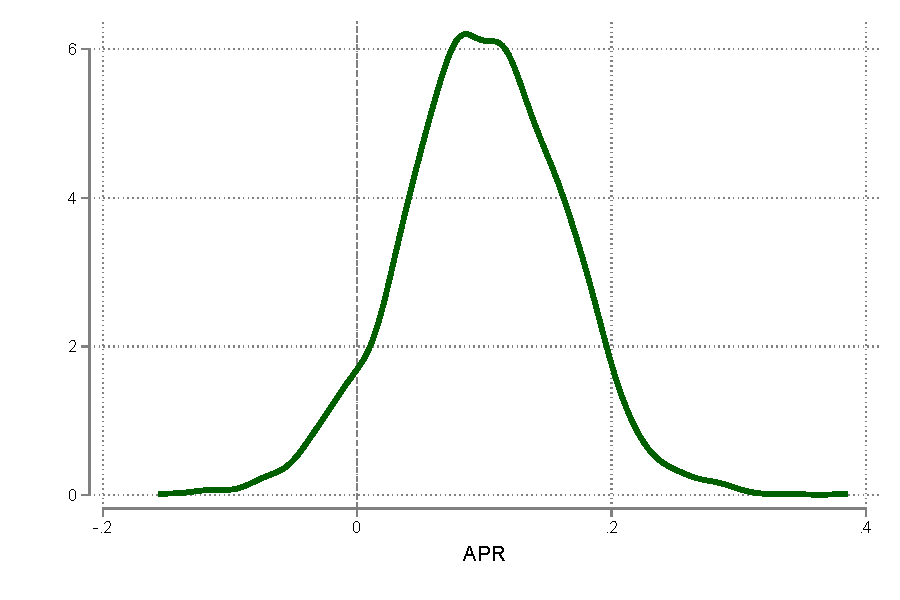
\includegraphics[width=\textwidth]{Figuras/he_dist_tau_hat_tut.pdf}
          \caption{Conditional TUT}
    \end{subfigure} 
       \begin{subfigure}{.35\textwidth}
        \centering
        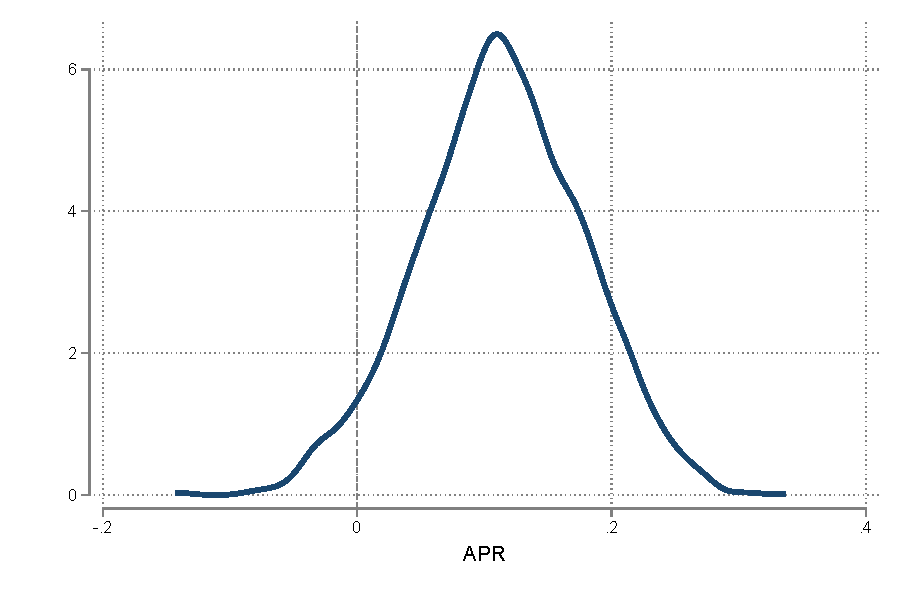
\includegraphics[width=\textwidth]{Figuras/he_dist_tau_hat_eff.pdf}
        \caption{Conditional ATE}
    \end{subfigure} 
    \end{center}
  \scriptsize{To estimate conditional average treatment effects given administrative and survey data and the function \texttt{causal\_forest()} of the \texttt{grf} R package; to estimate conditional TOT and TUT effects we use the \texttt{instrumental\_forest()} function from the same package. For more information see Appendix \ref{app:cate}.} 
  %\textit{Do file: }  \texttt{cate_dist.do}
\end{figure}


%\hfill \newline
%\noindent \textbf{Treatment effect distributions.} 
Figure \ref{heterogeneous_effects} plots densities of the estimated CATE, CTOT, and CTUT effects from the generalized random forest models described above.
In each case, the outcome variable is APR benefit, i.e.\ the reduction in APR from a structured payments contract.
As we see from the figure, the conditional average effects are highly heterogeneous but overwhelmingly positive. 
The TUT density is particularly interesting for the question of paternalism since, as emphasized above, it presents conditional average effects for borrowers who would not voluntarily choose structure.
Only 7\% of our estimated conditional TUTs are negative (95\% confidence interval of [4\%, 9\%]).\footnote{To be clear, this is a probability statement about conditional average effects over the distribution of covariates.
In particular, we estimate that  $\int \mathbbm{1}\{\mathbb{E}[Y_1 - Y_0| X = \mathbf{x}, C = 0] < 0\} \, f(\mathbf{x}|C=0) \, \mathrm{d}\mathbf{x}$ is approximately 0.07. The share of non-choosers with negative conditional \emph{average} treatment effects need not equal the share with a negative \emph{individual} effects, i.e.\ $\mathbbm{P}(Y_1 < Y_0| C = 0)$.
But the more treatment effect heterogeneity that $X_i$ explains, the closer these two values become.}
Figure \ref{heterogeneous_effects} strengthens the argument that many borrowers will save on financial cost by choosing the structured payment contract.



%\hfill \newline
%\noindent \textbf{``Mistake'' thresholds.} 
%Under the assumption that our instrumental forest estimates capture important sources of treatment effect heterogeneity, 
We now use the conditional TUT and TOT estimates described above to explore the extent to which borrowers in the choice arm could be said to have made a ``mistake'' by choosing to accept or refuse the structured repayment contract.
For the purpose of this exercise, we say that a non-chooser has made a ``mistake'' if her estimated CTUT is large and \emph{positive}: she did not select structured repayment, but our generalized random forest estimates suggest that someone with her observed characteristics would benefit from it, on average, in terms of lower financial costs.\footnote{Our sign convention defines treatment effects that \emph{benefit} borrowers as positive: a decrease in APR is a \emph{positive} treatment effect.} 
We write the word mistake in quotation marks to highlight that we are using this term as a convenient shorthand for a specific pattern of conditional average treatment effects rather than making the stronger claim that a certain borrower made a choice contrary to her own welfare. 
There are two reasons why ``mistakes'' may not fully capture welfare.
First, conditional average treatments are not equivalent to individual treatment effects: they only reflect observed sources of heterogeneity. 
The closer our covariates come to capturing the relevant sources of variation in individual treatment effects, the less of a concern this poses.
Second, our definition of a ``mistake'' does not incorporate all the costs and benefits that an individual borrower faces. 
Above we presented a number of robustness checks to address this concern in the context of \emph{unconditional} average treatment effects, addressing discounting, liquidity, and the costs of visiting the branch to make an interim payment, for example.
Here we take a similar but simpler approach in the case of \emph{conditional} average treatment effects, by considering ``mistakes'' at different APR \emph{thresholds}.
At any such threshold, we can calculate the percentage of non-choosers in the choice arm who have benefited by more than that threshold from having chosen structure, according to our CTUT estimates. 
Again: this does not directly measure welfare, only financial cost.

The green curve in Figure \ref{choose_wrong} presents the results of this analysis.
Defining $F_{\text{TUT}}(\delta)$ to be the CDF corresponding to the density of  CTUT estimates from Figure \ref{heterogeneous_effects}, the solid curve equals $[1 - F_{\text{TUT}}(\delta)] \times 100\%$ and the shaded region gives associated 95\% pointwise confidence bounds.
In words: for any given APR threshold on the horizontal axis, the vertical axis for the green curve plots the percentage of non-choosers who made a ``mistake'' 
 of at least that magnitude by \emph{not choosing} structured repayment.
Again: a mistake is defined as an estimated CTUT that exceeds the specified APR threshold. 

\vspace{.2in}
\begin{figure}[H]
 \caption{``Mistakes'' in the choice arm.}
\begin{center}
        \centering
        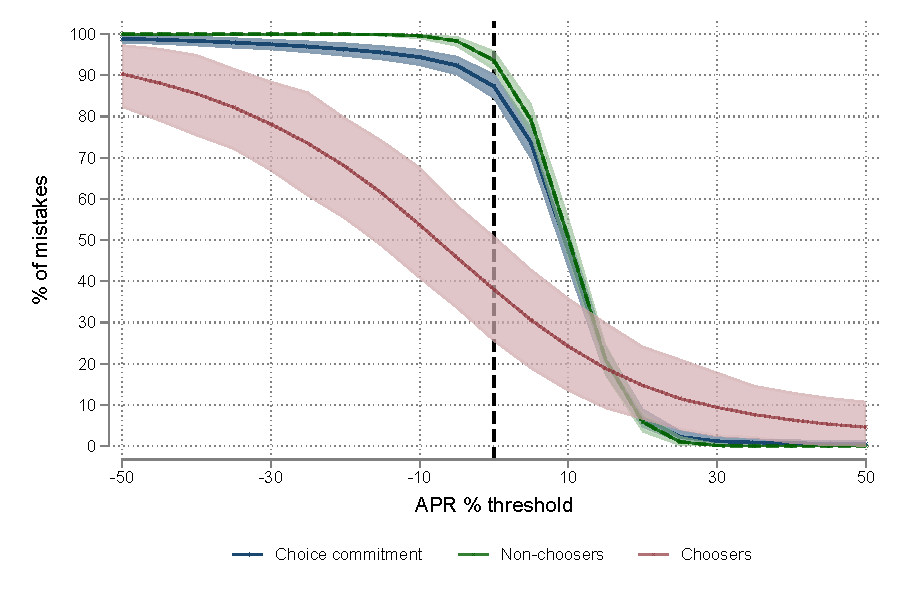
\includegraphics[width=0.65\textwidth]{Figuras/line_cw_apr_tot_tut.pdf}
 \end{center}       
 \scriptsize{
 %This figure presents conditional average TUT and TOT effects for the APR outcome from Figure \ref{heterogeneous_effects} in an alternative manner, to consider the fraction of borrowers in the choice arm who made ``mistakes'' in their decision to accept or refuse the structured contract. A ``mistake'' for a non-chooser is defined as a positive conditional TUT effect that significantly exceeds a specified threshold APR value.
 This figure plots the fraction of borrowers who made a ``mistake'' in their decision to except or refuse the structured contract, defined as a positive conditional TUT effect that exceeds a specified threshold APR value.
 %\textit{Do file: } \texttt{choose_wrong_quant_wrong_tot_tut.do}
 
%  The green curve equals $[1 - F_{\text{TUT}}(\delta)]\times 100\%$, where $F_{\text{TUT}}$ is the CDF corresponding to density of conditional TUT effects from Figure \ref{heterogeneous_effects}, computed using the instrumental forest approach from \cite{atheygrf}. Evaluated at any positive value on the horizontal axis, it gives the fraction of non-choosers in the choice arm who made a ``mistake'' by not choosing commitment. The green shaded region gives associated 95\% pointwise confidence bands. 
% Analogously, a ``mistake'' for a chooser is defined as a negative conditional TOT effect that exceeds a specified threshold APR value. The red curve equals $F_{\text{TOT}}(-\delta)$ where $F_{\text{TOT}}$ is the CDF corresponding to the density of conditional TOT effects from Figure \ref{heterogeneous_effects}. 
% The red shaded region gives associated 95\% pointwise confidence bands.
% For both the red and green curves, we define the APR threshold so that larger mistakes are to the \emph{right} of smaller mistakes.
% This allows us to construct the overall fraction of mistakes in the choice arm, the blue curve, as a weighted average of the green and red curves.
% The weights equal the share of choosers and non-choosers in the choice arm.
}
    \label{choose_wrong}
\end{figure}

We can carry out an analogous exercise using our estimated CTOT to explore ``mistakes'' by choosers in the choice arm, subject to the same caveats as above.
Here the situation is reversed.
We say that a chooser has made a ``mistake'' if her estimated CTOT is large and \emph{negative}: she chose structured repayment, but our generalized random forest estimates suggest that someone with her observed characteristics would face \emph{higher} financial costs, on average, with structure.\footnote{Our sign convention defines treatment effects that \emph{harm} borrowers as positive: an \emph{increase} in APR is a \emph{negative} treatment effect.}
As we did for the non-choosers, we consider alternative APR thresholds to define ``mistakes''.
For example, we can ask: what fraction of non-choosers would have faced an APR that was at least 10 percentage points more favorable if they \emph{had not} chosen structured repayment?
The red curve in Figure \ref{choose_wrong} presents the results of this analysis.
The solid curve equals $F_{\text{TOT}}(-\delta)$ where $F_{\text{TOT}}$ is the CDF corresponding to the density of conditional TOT effects from Figure \ref{heterogeneous_effects}, while the red shaded region gives pointwise 95\% confidence bands.
Note that we use a \emph{positive} APR threshold to denote a mistake for both choosers (red) and non-choosers (green).
This ensures that bigger mistakes are always to the \emph{right} of smaller mistakes and allows us to plot both curves in a single figure.
In other words a \emph{positive} value of $\delta$ always denotes a mistake of a given magnitude, regardless of whether we are considering choosers or non-choosers.
This convention allows us to compute present the \emph{overall} percentage of borrowers in the choice arm who made a ``mistake'' of a particular magnitude by taking a weighted average of the green and red curves: see the blue solid curve and associated pointwise 95\% confidence bands in Figure \ref{choose_wrong}.
The blue curve is very similar to the green curve because 89\% of borrowers in the choice arm are non-choosers.


%For choosers we follow an analogous approach, defining a ``mistake'' as a \emph{negative} CTOT exceeding a particular APR threshold.
%The results for choosers can be read from the red curve in Figure \ref{choose_wrong}.
%If $F_{\text{TOT}}(\delta)$ denotes the CDF corresponding to the density of conditional TOT estimates from Figure \ref{heterogeneous_effects}, then the red curve is merely $\left[1 - F_{\text{TOT}}(\delta)\right] \times 100\%$.
%In other words, the red curve gives the percentage of choosers who made a ``mistake'' when mistakes are defined at a particular APR threshold.
%The red shaded region gives associated 95\% pointwise confidence bounds.

The results in Figure \ref{choose_wrong} suggest that a large fraction of non-choosers would have experienced lower financial costs had they chosen the structured payment contract, even at an APR threshold as large as 10 percentage points, we estimate that more than half of them should have chosen the structured payment contract to lower financial costs.
In contrast, comparatively fewer choosers appear to have made mistakes by choosing structure, although our estimates for this group are more imprecise.
This now allows us to make a stronger statement in favor of paternalism in our context; not only does structure generate large benefits \textit{on average}, but it also benefits the \emph{vast majority} of borrowers who would be coerced under a policy of mandatory structure.  Indeed, in Appendix \ref{targeting} we show that given the relatively weak power of reliably collectible covariates in predicting variation in the TOT and TUT, an optimal feasible model of targeting results in only very minimal decreases in the fraction of the sample assigned to the `wrong' treatment relative to simply assigning everyone to mandated structure (the CATE estimates above suggest 9.8\% of the sample is harmed by universally mandated structure, and this fraction falls only to 9.6\% with optimal feasible targeting).  Hence in this context there seems to be limited downside for borrowers in simply shifting the default contract for everyone.  



    
\section{Conclusion} \label{conclusion}

This paper makes several contributions. First, it analyzes the important but understudied industry of pawn loans. Likely, hundreds of millions of people use pawn loans, and yet few economic studies exist.   We provide new stylized facts about pawn lending, and provide evidence as to how contract structure in this context drives repayment and borrower costs.  We do this using a novel ``Mandates-Choice'' design, which paired with twin exclusion restrictions allows us to go beyond ATE results and draw an important set of conclusions about the relationship between take-up and heterogeneous treatment effects, providing a complement to marginal treatment effects methods. We show that a simple change to contract terms results in substantial financial savings for pawn borrowers: mandatory structure lowers the APR from 57\% to 46\%, and reduces the fraction of borrowers who default by 6.6 pp, or 15\%. 


In terms of relating impacts to selection we find substantial benefits of treatment for non-choosers and no evidence of selection on gains. This is the first such result in the household finance literature.  Estimating treatment effects for non-takers is critical in thinking about paternalism, and we show one rigorous way to do it that is new in the literature and distinct from Karlan-Zinman designs. 
 The over-collateralization of pawn loans is a  potential explanation for why this relatively simple repayment-inducing contract is not offered (or required) in the status quo.  Given that lender profits are higher under default, this may be a case of the `veiled paternalism' from \cite{Laibson2018} turned on its head:  principals \textit{do not} embed commitment into contracts in a manner that is not obvious to agents but shifts behavior in a manner that improves returns for the principal.  



We correlate TUT impacts with behavioral parameters to try to explain the fact that only 11\% of borrowers choose structured payments when virtually all of them would benefit from it.  Our results suggest that over-optimism of pawn recovery is the characteristic most strongly associated with benefiting from the commitment despite not having chosen it, and may be an explanation for the low demand for structured repayment. Low take-up suggests that in order to achieve widespread benefits in this context compulsory structure appears to be an attractive policy. With a now well-established toolkit of regular small payments and incentives delivering small default rates in microfinance, regulators may fruitfully investigate the possibility of requiring pawnbrokers to embed features of commitment and regularity into their repayment structures in more consistent ways.



%\textcolor{red}{Overcollateralization and sunk payments make pawn loans a product different than microfinance and payday loans in the incentives they create. In fact, while recent literature shows that more flexibility in payments may be beneficial in microfinance, this does not seem to be the case in our pawn lending context.} That this new contract generated large benefits for borrowers and yet was not offered, and that a contract that generated default was the industry standard instead, is related to the idea of ``veiled paternalism'' \cite{Laibson2018}, put on its head, %In ``veiled paternalism'' principals embed forms of commitment into their products but mask this fact from consumers who may need but do not desire commitment, in pawn lending, over-collateralization means that lenders stand to make more money from defaulting borrowers, generating incentives for ``veiled \textit{non}-paternalism,'' embedding features that lead to high borrower costs.

%Potentially due to the nature of the borrower pool, 
%In our context voluntary commitment choice does improve borrower outcomes, but forcing commitment did induce significant cost savings for the overall group of clients.  




%Why do borrowers leave such substantial returns on the table? 

%Our borrower pool overestimates their probability of repayment by more than 50\%, and our positive TUT estimate is largely confined to borrowers who incorrectly believe that they have little chance of defaulting.  %More standard explanations such as discounting, learning, or time inconsistency find little support in our data. 

%Using machine learning methods, we find the benefits of commitment close to universal. The benefits of targeting commitment based on characteristics that lenders can observe and participants would truthfully reveal are extremely limited, suggesting that universal commitment is an attractive policy in our empirical setting. 

%Where lenders have no incentive to engage in veiled paternalism and customers display inefficiently low demand for it, financial policy regulation may prove an attractive option.  Pawnshops, along with other over-collateralized credit products such as payday lending, exist in an environment where the lender may desire customers to lose their collateral on the loan, hurting especially low-income populations who are its main users. With a now well-established toolkit of regular small payments and incentives delivering small default rates in microfinance, regulators may fruitfully investigate the possibility of requiring pawnbrokers to embed features of commitment and regularity into their repayment structures in more consistent ways.\footnote{If employed at scale in a competitive lending sector this would redistribute welfare from those who would have repaid (whose interest rates must now rise to cover lower returns from collateral seizure) towards those who would only repay in the presence of commitment. In a setting of lender market power however, redistribution from lenders to borrowers could occur.}

There are several questions left for future research. Would results hold using more comprehensive measures of welfare? How fast would borrowers learn about the benefits of structured payments if regulators forced lenders to provide this contractual feature? How would lender competition affect the incentives to provide such a contract? Much needs to be done to improve the lives of the millions of borrowers using pawn loans.

%%%%%%%%%%%%%%%%%%%%%%%%%%%%%%%%%%%%%%%%%%%%%%%%%%%%%%%%%%%%%
%BIBLIOGRAPHY
\begingroup
\setstretch{1.10}
\bibliographystyle{authordate1}
%\bibliographystyle{amsalpha}
%\bibliographystyle{AER}

\bibliography{References}
\endgroup

%%%%%%%%%%%%%%%%%%%%%%%%%%%%%%%%%%%%%%%%%%
% Proofs below
%%%%%%%%%%%%%%%%%%%%%%%%%%%%%%%%%%%%%%%%%%
\appendix

\section{Proofs}
\label{sec:proofs}

This section gives a formal derivation of the identification results presented in Equations \eqref{eq:TOT}--\eqref{eq:ASL} of \autoref{sec:randchoice}.
To simplify the presentation, we omit $i$ subscripts throughout.
%and adopt the shorthand  $Z_0 \equiv \mathbbm{1}(Z=0)$, $Z_1 \equiv \mathbbm{1}(Z=1)$, and $Z_2 \equiv\mathbbm{1}(Z=2)$.
%The following assumption collects our exclusion restriction and the key features of the constrained choice design.

\begin{assumption}[Randomized Choice Design and Exclusion Restriction]\mbox{}
\label{assump:randchoice}
   \begin{enumerate}[(i)]
   \item $Z$ is independent of $(Y_{0}, Y_{1}, C)$
   \item $D = \mathbbm{1}(Z \neq 2)Z + \mathbbm{1}(Z = 2)C$
   \item $Y = \mathbbm{1}(Z = 0) Y_{0} + \mathbbm{1}(Z = 1) Y_{1} + \mathbbm{1}(Z = 2) [ (1 - C) Y_{0} + C Y_{1}]$
   \end{enumerate}
\end{assumption}

\begin{lem}
Under Assumption \ref{assump:randchoice},
\label{lem_randchoice}
   \begin{enumerate}[(i)]
       \item $\mathbbm{E}(D|Z=2) = \mathbb{P}(C=1)$
       \item $\mathbbm{E}(Y|Z=0) = \mathbbm{E}(Y_0)$
       \item $\mathbbm{E}(Y|Z=1) = \mathbbm{E}(Y_1)$
       \item $\mathbbm{E}(Y|D=0,Z=2) = \mathbbm{E}(Y_0|C=0)$
       \item $\mathbbm{E}(Y|D=1,Z=2) = \mathbbm{E}(Y_1|C=1)$.
   \end{enumerate} 
\end{lem}

\begin{proof}
Part (i) follows because $Z=2$ implies $D=C$ and $Z$ is independent of $C$.  
Parts (ii) and (iii) follow similarly: given $Z=0$ we have $Y = Y_0$, given $Z=1$ we have $Y = Y_1$, and $Z$ is independent of $(Y_0,Y_1)$.
For parts (iv) and (v), first note that Assumption \ref{assump:randchoice} (iii) implies that $Z$ is conditionally independent of $(Y_0,Y_1)$ given $C$.
Now, $Z=2$ implies that $D=0$ if and only if $C=0$. Hence, $\mathbbm{E}(Y|D=0, Z=2) = \mathbbm{E}(Y_0|C=0)$ establishing part (iv).
For part (v) $Z=2$ implies that $D=1$ if and only if $C=1$ from which it follows that $\mathbbm{E}(Y|D=1, Z=2) = \mathbbm{E}(Y_1|C=1)$.
\end{proof}

\begin{prop} 
Under Assumption \ref{assump:randchoice},
    \begin{enumerate}[(i)]
        \item $\text{TOT} \equiv \mathbbm{E}(Y_1 - Y_0|C=1)  = \displaystyle \frac{\mathbbm{E}(Y|Z=2) - \mathbbm{E}(Y|Z=0)}{\mathbbm{E}(D|Z=2)}$
        \item $\text{TUT} \equiv \mathbbm{E}(Y_1 - Y_0|C=0) = \displaystyle \frac{\mathbbm{E}(Y|Z=1) - \mathbbm{E}(Y|Z=2)}{1 - \mathbbm{E}(D|Z=2)}$
        \item $\text{ASB} \equiv \mathbbm{E}(Y_0|C=1) - \mathbbm{E}(Y_0|C=0) = \displaystyle \frac{\mathbbm{E}(Y|Z=0) - \mathbbm{E}(Y|Z=2,D=0)}{\mathbbm{E}(D|Z=2)}$
        \item $\text{ASL} \equiv \mathbbm{E}(Y_1|C=1) - \mathbbm{E}(Y_1|C=0) = \displaystyle \frac{\mathbbm{E}(Y|Z=2,D=1) - \mathbbm{E}(Y|Z=1)}{1 - \mathbbm{E}(D|Z=2)}$.
    \end{enumerate}
\end{prop}

\begin{proof}
Parts (i) and (iii) we require an expression for $\mathbbm{E}(Y_0|C=1)$ in terms of $(Y, D, Z)$.
By Lemma \ref{lem_randchoice}(ii) and iterated expectations 
\[
\mathbbm{E}(Y|Z=0) = \mathbbm{E}(Y_0) = \mathbbm{E}(Y_0|C=0) \mathbbm{P}(C=0) + \mathbbm{E}(Y_0|C=1) \mathbbm{P}(C=1).
\]
Re-arranging and substituting Lemma \ref{lem_randchoice}(i) and (iv),
\begin{align}
\mathbbm{E}(Y_0|C=1)  
%&= \frac{\mathbbm{E}(Y|Z=0) - \mathbbm{E}(Y_0|C=0) \mathbbm{P}(C=0)}{\mathbbm{P}(C=1)}\nonumber\\ 
&=  \frac{\mathbbm{E}(Y|Z=0) - \mathbbm{E}(Y|Z=2,D=0) \mathbbm{E}(1 - D|Z=2)}{\mathbbm{E}(D|Z=2)}.
\label{eq:Y0C1}
\end{align}
Part (i) follows by combining \eqref{eq:Y0C1} with Lemma \ref{lem_randchoice}(v) and simplifying; part (iii) follows by combining \eqref{eq:Y0C1} with Lemma \ref{lem_randchoice}(iv) and simplifying.
Similarly, for parts (ii) and (iv) we require an expression for $\mathbbm{E}(Y_1|C=0)$ in terms of observables.
By Lemma \ref{lem_randchoice}(iii) and iterated expectations,
\[
\mathbbm{E}(Y|Z=1) = \mathbbm{E}(Y_1) = \mathbbm{E}(Y_1|C=0)\mathbbm{P}(C=0) + \mathbbm{E}(Y_1|C=1) \mathbbm{P}(C=1).
\]
Re-arranging and substituting Lemma \ref{lem_randchoice}(i) and (v),
\begin{align}
\mathbbm{E}(Y_1|C=0) 
%&= \frac{\mathbbm{E}(Y|Z=1) - \mathbbm{E}(Y_1|C=1)\mathbbm{P}(C=1)}{\mathbb{P}(D=0)} \nonumber\\
&=\frac{\mathbbm{E}(Y|Z=1) - \mathbbm{E}(Y|Z=2,D=1)\mathbbm{E}(D|Z=2)}{\mathbb{E}(1-D|Z=2)}.
\label{eq:Y1C0}
\end{align}
Part (ii) follows by combining \eqref{eq:Y1C0} with Lemma \ref{lem_randchoice}(iv) and simplifying; part (iv) follows by combining \eqref{eq:Y1C0} with Lemma \ref{lem_randchoice}(v) and simplifying.
\end{proof}

\newpage


%%%%%%%%%%%%%%%%%%%%%%%%%%%%%%%%%%%%%%%%%%%%%%%
\setcounter{table}{0}
\setcounter{figure}{0}
\setcounter{section}{0}
\pagenumbering{gobble}
% APPENDIX 
\pagenumbering{arabic}
\renewcommand\thefigure{OA-\arabic{figure}}
\renewcommand\thetable{OA-\arabic{table}}
\renewcommand*{\thepage}{OA - \arabic{page}}
\renewcommand\thesection{Appendix \Alph{section}.}
\renewcommand\thesubsection{\Alph{section}.\arabic{subsection}}

\newgeometry{margin=1in}
\begin{center}
	\Large ONLINE APPENDIX: The forcing-choice design and paternalism in pawnshop borrowing \\[0.5em]
	%\Large{Appendix $-$ For Online Publication} \\[1em]
	\large \author{Craig McIntosh \and Isaac Meza \and Joyce Sadka \and Enrique Seira \and Francis J.\ DiTraglia}
\end{center}


\begin{appendix}

    
%\section{ Treatment Explanation Materials and Pictures}
\section{Additional materials} 
%\vspace{.2in}

\begin{figure}[!h]
     \caption{Behavior of borrowers who lost their pawn.}
    \begin{center}
    \begin{subfigure}{0.35\textwidth}
        \caption{Elapsed days to first payment}
        \centering
        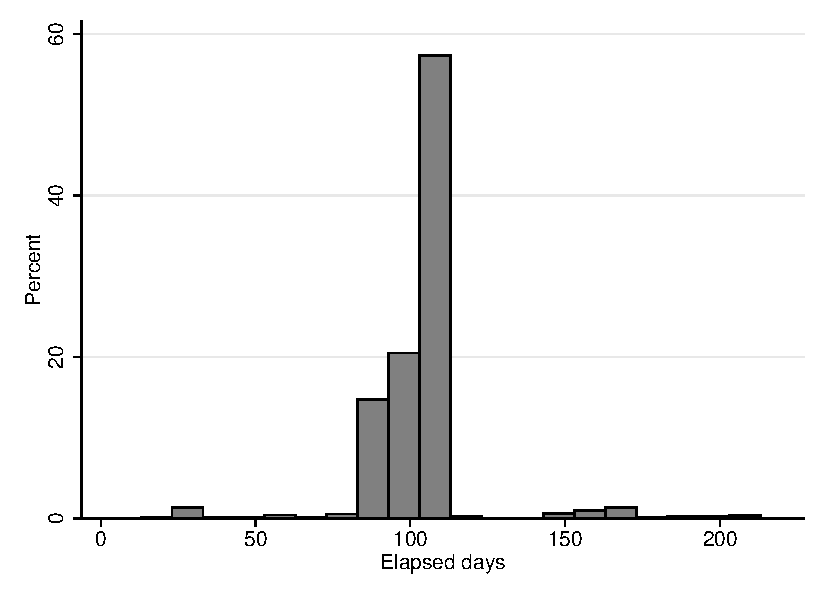
\includegraphics[width=\textwidth]{Figuras/hist_firstdays_default.pdf}
    \end{subfigure}
    \begin{subfigure}{0.35\textwidth}
        \caption{Elapsed days to last payment}
        \centering
        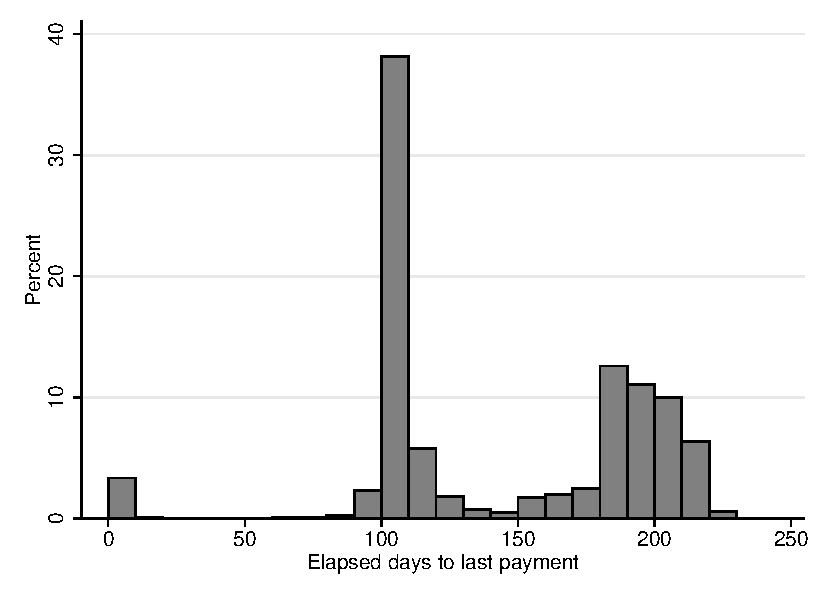
\includegraphics[width=\textwidth]{Figuras/hist_days_default.pdf}
    \end{subfigure}
        \begin{subfigure}{0.35\textwidth}
        \caption{Payments as \% of loan}
        \centering
        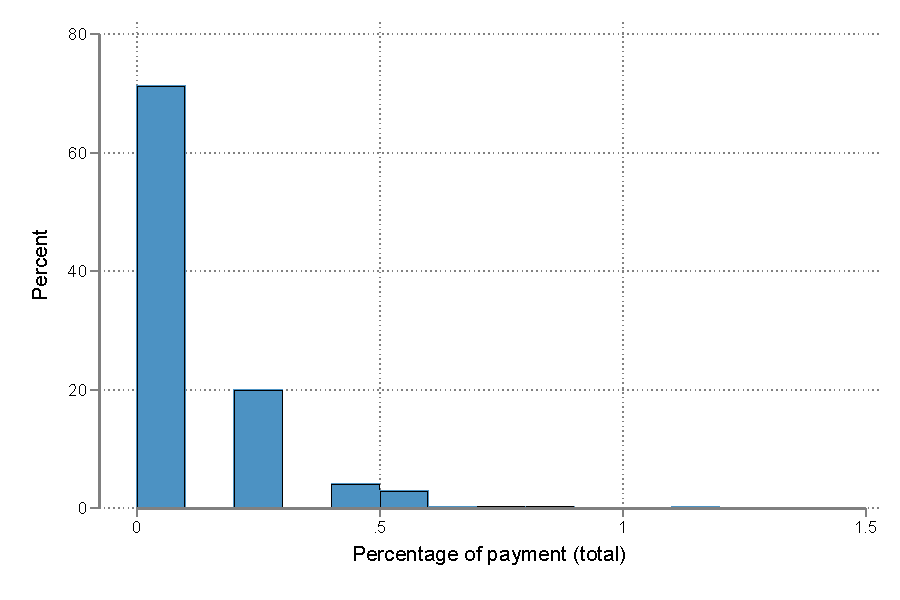
\includegraphics[width=\textwidth]{Figuras/hist_percpay_default.pdf}
    \end{subfigure}
    \begin{subfigure}{0.35\textwidth}
        \caption{Number of payments}
        \centering
        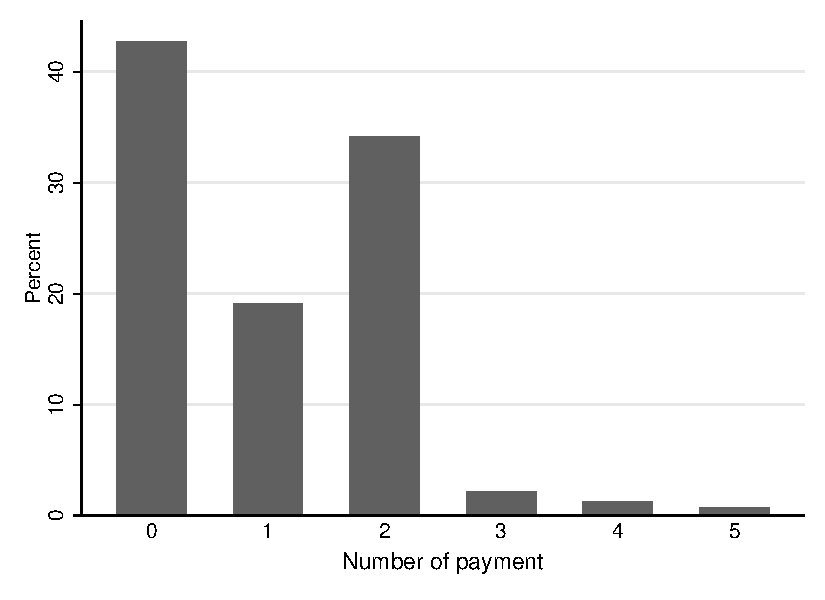
\includegraphics[width=\textwidth]{Figuras/hist_numpay_default.pdf}
    \end{subfigure}
    \end{center}
        \footnotesize{This figure provides more details on the behavior of clients who were assigned to the control group and did not recover their pawn. Panel (a) shows a histogram of days elapsed from the pawn to the first payment, while panel (b) displays a histogram of days elapsed until the last payment. Some borrowers make payments after day 105, the end of the grace period: if they pay all interest owed, they can ``restart'' the loan. This amounts to starting a new loan with the same conditions and same pawn. Panel (c) shows a histogram of the fraction of the loan paid, while panel (d) presents a barplot of the number of times that borrowers went to the branch to make payments.}
        \label{proxy_naive}
      %\textit{Do file: }  \texttt{hist\_den\_default.do}
\end{figure}

\begin{figure}[H]
    \caption{Weekly default rates experimental branches and all branches}
    \label{external_validity}
    \begin{center}
    \begin{subfigure}{0.65\textwidth}
        \centering
        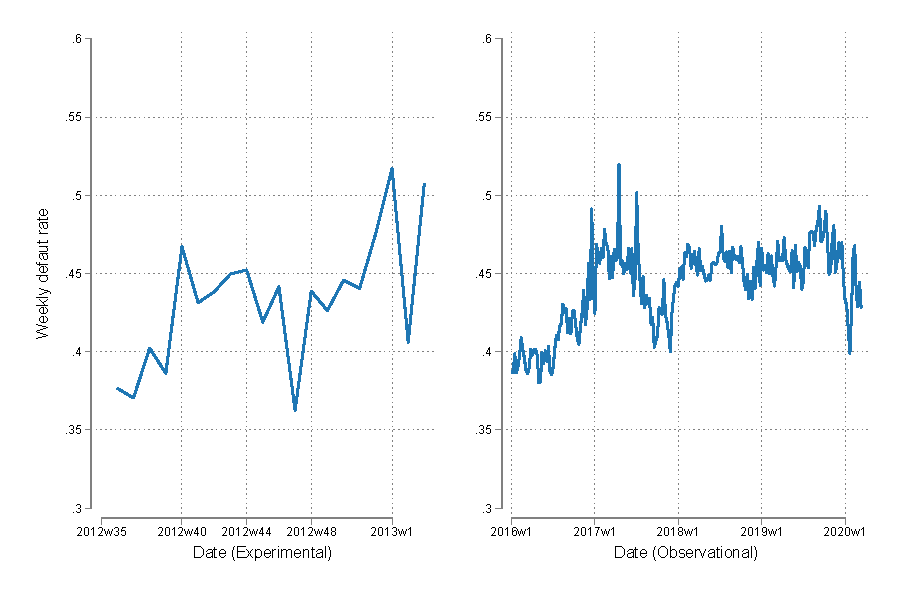
\includegraphics[width=\textwidth]{Figuras/weekly_def_rates.pdf}
    \end{subfigure}
    \end{center}
\footnotesize{The above figure shows the weekly default rates for our experimental sample, and for 4 years after our experiment. We show that the default rates in the experimental sample are not atypical. }
    \label{weekly_def_rates}
%\textit{Do file: } \texttt{determinants_choice.do}       
\end{figure}


\normalsize
%Really force it to normal size and linespread
\normalsize


\begin{figure}[H]
    \caption{Determinants of choice.}
    \begin{center}
    \begin{subfigure}{0.65\textwidth}
        \centering
        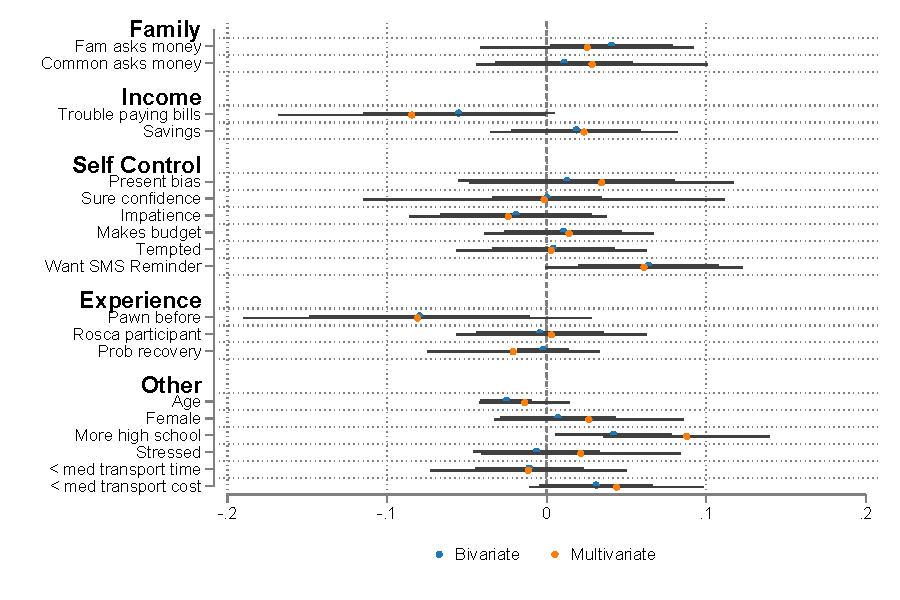
\includegraphics[width=\textwidth]{Figuras/determinants_choose_commitment.pdf}
    \end{subfigure}
    \end{center}
\footnotesize{The above figure shows the determinants in a bivariate and multivariate OLS regression of choosing commitment. Choice commitment is a binary variable equal to one, whenever subjects choose the forced commitment contract in the choice arm. }
    \label{determinants_choose}
%\textit{Do file: } \texttt{determinants_choice.do}       
\end{figure}

\newpage

\begin{table}[!h]
\caption{Baseline survey questions (translated to English)}
\label{baseline_survey}
\begin{center}
\scriptsize{% Table generated by Excel2LaTeX from sheet 'transcribed'
\begin{tabular}{cl}
\toprule
      & \textbf{Baseline Survey} \\
\midrule
\midrule
1     & \textbf{Your pawn was:} \\
      & (a) Inherite, (b) a gift, (c) bought by me, (d) lend to me, (e) other \_\_\_\_\_\_\_\_\_\_\_\_ \\
2     & \textbf{Mark with an "X" in the line below how likely is that you recover your pawn. } \\
      & \textbf{Where 0 is impossible and 100 is completely certain} \\
3     & \textbf{How much do you think the item you plan to pawn is worth?       \_\_\_\_\_\_\_\_\_\_\_\_\_\_ pesos} \\
4     & \textbf{Gender      } \\
5     & \textbf{Age} \\
6     & \textbf{Civil Status } \\
      & (a) married, (b) single, (c) divorced, (d) widowed \\
7     & \textbf{Work status} \\
      & (a) employed, (b) own business, (c) houseshores, (d) don't work, (e) retired, (f) study \\
8     & \textbf{Education} \\
      & (a) no formal education, (b) primary, (c) middle school, (d) highschool, (e) more than highschool \\
9     & \textbf{In the last month, did a friend or family member asked you for money?} \\
      & (a) yes  (b) no \\
10    & \textbf{What would you like to have: 100 pesos tomorrow or 150 pesos in one month?} \\
11    & \textbf{How often do you feel stressed by your economic situation?} \\
      & (a) always, (b) very often, (c) sometimes, (d) never \\
12    & \textbf{What is the main reason you want to pawn?} \\
      & (a) Need the money because somebody in my family lost his/her job \\
      & (b) Need the money to pay for a sickness in the family \\
      & (c) Need the money for an urgent expense \\
      & (d) Need the money for some non urgent expense. \\
13    & \textbf{How stressed do you feel from the situation that led to to pawn?} \\
      & (a) very stressed, (b) somwhat stressed, (c) a little stressed, (d) not stressed  \\
14    & \textbf{In 3 months, I expect to have a  \_\_\_\_\_\_\_\_\_\_\_\_\_\_\_\_ situation} \\
      & (a) better, (b) similar,  (c) worse \\
15    & \textbf{Have you panwned before?} \\
      & (a) yes  (b) no \\
16    & \textbf{How many times have you pawned on a Lender P branch?} \\
      & (a) NO\_\_\_    (b)  1-2 times \_\_\_    (c) 3-5 times\_\_\_\_   (d) More than 5\_\_\_\_ \\
17    & \multicolumn{1}{p{54.91em}}{\textbf{If you are saving money and a family member wants to use it for something }} \\
      & \multicolumn{1}{p{54.91em}}{(a) I would only give him the money for an urgent expenze} \\
      & \multicolumn{1}{p{54.91em}}{(b) I would give him the money even if it was not an urgent expense} \\
      & \multicolumn{1}{p{54.91em}}{(c) I would not give him/her the money regardless} \\
      & \multicolumn{1}{p{54.91em}}{(d) No one would ask me for my money} \\
18    & \textbf{Do you make an expenses budget for the month ahead of time?} \\
      & (a) always, (b) very often, (c) sometimes, (d) never \\
19    & \multicolumn{1}{p{54.91em}}{\textbf{Do you have other items you could pawn?}} \\
      & (a) yes  (b) no \\
20    & \textbf{Do you have savings?} \\
      & (a) yes  (b) no \\
21    & \textbf{Do you participate in a ROSCA?} \\
      & (a) yes  (b) no \\
22    & \textbf{Is it common that family or friends ask for money?} \\
      & (a) yes  (b) no \\
23    & \textbf{How much did you spend to come to the branch today?    \$\_\_\_\_\_\_\_\_\_\_\_\_\_\_ pesos} \\
24    & \textbf{How much time does it usually take to come to this branch?    \_\_\_\_\_\_\_\_\_\_\_} \\
25    & \textbf{How much does your family spend in a normal week?   \$\_\_\_\_\_\_\_\_\_\_\_\_\_\_ pesos} \\
26    & \textbf{How much do you manage to save in a normal week?   \$\_\_\_\_\_\_\_\_\_\_\_\_\_\_ pesos} \\
27    & \textbf{Does it happen to you that you spend more than you wanted because you fall into temptation?} \\
      & (a) never, (b) almost never, (c) sometimes, (d) very often \\
28    & \textbf{In the last 6 months, has it happened that at some point you lacked money to pay} \\
      & (a) rent?    (b) food    (c)food   (d) medicine  (e) electricity   (f) heating   (g) telephone    (i) water \\
29    & \textbf{What would you like to have: 100 pesos in 3 months or 150 pesos in four months?} \\
30    & \textbf{Would you like to receive (free) reminders for upcomming payments?} \\
      & (a) yes  (b) no \\
\bottomrule
\end{tabular}%
}
\end{center}
\scriptsize{
Translation of the baseline questionnaire. Highlighted questions were used in the wide forest.}
\end{table}

\newpage

\begin{landscape}
\subsection{Intermediate Outcomes}
  
\begin{table}[!h]
\caption{Effects on intermediate outcomes}
\label{mechanisms}
\begin{center}

\scriptsize{% Table generated by Excel2LaTeX from sheet 'mechanism'
\begin{tabular}{lccccccc}
\toprule
      & \% of payment in 1st visit & $\Pr($Recovery in 1st visit) & \% of payment & $\Pr($+ payment \& default) & \% of pay $|$ def  & $\Pr($Selling pawn) & $\Pr($Selling pawn $|$ def) \\
\midrule
\midrule
      & (1)   & (2)   & (3)   & (4)   & (5)   & (6)   & (7) \\
\midrule
\midrule
Forced commitment & 7.92*** & 0.079*** & 9.43*** & -0.070*** & -3.90*** & 0.0050 & 0.14*** \\
      & (2.78) & (0.026) & (2.62) & (0.015) & (1.26) & (0.021) & (0.034) \\
Choice commitment & -0.97 & -0.010 & 1.40  & -0.026* & -1.75* & 0.0035 & 0.049* \\
      & (2.20) & (0.022) & (2.36) & (0.013) & (1.00) & (0.019) & (0.029) \\
      &       &       &       &       &       &       &  \\
\midrule
Observations & 6304  & 6304  & 6304  & 6304  & 2488  & 6304  & 2488 \\
R-squared & 0.014 & 0.016 & 0.015 & 0.011 & 0.022 & 0.016 & 0.033 \\
Control Mean & 44.7  & 0.30  & 67.2  & 0.12  & 9.46  & 0.31  & 0.72 \\
\midrule
\midrule
      &       &       &       &       &       &       &  \\
\midrule
      & Days to 1st payment & \# of visits & \# of visits $|$ recovery & \# of visits $|$ def & Loan duration (days) & Loan duration $|$ recovery &  \\
\midrule
\midrule
      & (8)   & (9)   & (10)  & (11)  & (12)  & (13)  &  \\
\midrule
\midrule
Forced commitment & -13.8*** & -0.031 & -0.19*** & 0.062 & -27.9*** & -17.9*** &  \\
      & (1.61) & (0.049) & (0.049) & (0.053) & (4.35) & (3.88) &  \\
Choice commitment & -3.51** & 0.085 & -0.077* & 0.13** & -0.18 & -1.35 &  \\
      & (1.57) & (0.053) & (0.041) & (0.063) & (4.33) & (4.19) &  \\
      &       &       &       &       &       &       &  \\
\midrule
Observations & 4412  & 6304  & 2488  & 3031  & 6304  & 3031  &  \\
R-squared & 0.055 & 0.022 & 0.025 & 0.018 & 0.054 & 0.041 &  \\
Control Mean & 82.8  & 1.14  & 0.39  & 1.44  & 136.6 & 103.9 &  \\
\bottomrule
\bottomrule
\end{tabular}%
}

\end{center}
\footnotesize{This table explores treatment effects in ``intermediate variables''. Each column represents regression output for different dependent variables following equation (\ref{basic_reg}). Panel A focuses on variables related to the speed of payment. While Panel B focuses on variables related to default, and Panel C related to visits. 
% The outcome variables are as follows:  number of days elapsed between origination and first payment (col 1); percentage of the loan paid in the first payment (col 2); probability of recovery in the first visit (col 3); loan duration is the number of days the borrower took to payoff her loan for those that recover, the number of days until default for those that default, and the maximum number of days we observe them in the sample for those that have not recovered or defaulted (col 4); loan duration conditional on recovery; an indicator for paying a positive amount towards recovery but nonetheless losing the pawn (col 6); the percentage or the loan paid, conditional on defaulting --`wasted payments' (col 7). Column 8 uses the phrase `selling the pawn' for a dummy variable indicating the borrower did not pay any amount towards recovery and lost the pawn. Moreover, (col 9) shows that treatment effects are concentrated in the intensive margin as treatment does not affect the fraction of clients who pay a positive amount towards pawn recovery. The dependent variable in column 10 is the number of day-visits to the branch (measured by the existence of transactions that day associated with our particular pawn), while column 11 conditions on borrowers that lost the pawn.
Each regression includes branch and day-of-week FE. Standard errors are clustered at the branch-day level.}
%\textit{Do file: } \texttt{mechanisms.do}
\end{table}
\end{landscape}

\normalsize
%Really force it to normal size and linespread
\normalsize



\subsection{Censoring} \label{App_censoring}


Some loans in our sample are ``censored'' in that they continue beyond our observation period.  For these loans, we do not know whether the borrower ultimately defaulted or recovered her pawn.   We have also shown that one effect of the forcing arm is to accelerate repayment, meaning that it is less likely for loans in this arm to be censored.  This issue is illustrated in Figure \ref{survival_graph}, which shows the CDF of loan completion (either default or recovery in Panel (a)) and loan recovery (Panel (b)) by the number of days since first pawn.  Two features of these graphs are salient for our analysis.  The first is the extent to which loan outcomes are observed more quickly in the forced commitment arm.  This is primarily due to the substantially higher rate of repayment of Forced Commitment loans at 120 days (15 pp higher than the other arms).  The second is the very low rate at which loans are recovered in any arm after 120 days.  In the 180-320 day window loans are largely dormant, suggesting that many of the censored loans will in fact end in default.

The confluence of censoring and a treatment effect on censoring is potentially problematic from an experimental point of view.  The approach taken in the headline results is a conservative one in that it inherently assumes that all of the loans outstanding at the end of the observation window will be repaid, making it so that the acceleration of payment observed in the Forced arm does not translate mechanically into the that treatment decreasing default.  Nonetheless, to be certain that this issue is not driving our results we conduct a bounding exercise to understand how large the effects of this problem can possibly be.  

One way of considering the effect that this issue could have on our results is to make extreme assumptions about the outcome of these loans in the treatment and control so as to bound the possible influence of censoring. In Table \ref{bounding_censoring} we compare the Forced and Control arms, bounding the censoring issue by reversing assumptions about the outcome of censored loans in the treatment versus the control.   Panel B provides the lower bound for the treatment effect (closest to zero) by assuming censored control loans are always repaid and treatment loans never are; even in this lower-bound case the treatment effect is cost-reducing and significant at the 1\% significance level and indeed the magnitude of this lower bound estimate is only 6\% closer to zero than our headline result.   Panel C estimates the upper bound by making the reverse assumption.  Comfortingly, even with these extreme assumptions the significance on the main treatment effects never flips and treatment effects on financial cost and interests payments remain negative and significant in all scenarios.  So there appears to be no scope for the censoring issue to overturn our main results. 

Finally, Panel E of this table conducts a logit prediction model that uses all of the available information on loans that were completed to predict the outcome of loans that were not.  This is a ``best guess'' of the outcome on censored loans.  Using this prediction, we replicate the main experimental results and find that the treatment effect on financial cost increases from -204 (main results) to -264 (censored loans predicted), and the APR from -11\% to -17\%.  Hence, while the censoring issue does have an effect on the magnitude of our estimated treatment effects, these  checks confirm that (a) the core results are fully robust to censoring, and (b) the headline approach that we take to the issue is conservative and likely understates the true magnitude of impacts.





\begin{table}[H]
\caption{Bounding censoring} 
\label{bounding_censoring}
\begin{center}
\resizebox{0.75\textwidth}{!}{
\footnotesize{% Table generated by Excel2LaTeX from sheet 'censoring_imp'
\begin{tabular}{lcccccc}
\toprule
      & FC    & Interest pymnt & Principal pymnt & Lost pawn value & Default & APR \\
\midrule
      & \multicolumn{6}{c}{Panel A : $\quad$ Control  = 0           $\quad\quad$                  Forced Commitment = 0} \\
\midrule
\midrule
      & (1)   & (2)   & (3)   & (4)   & (5)   & (6) \\
\midrule
\midrule
Forced commitment  & -236.0*** & -191.7*** & -0.63 & -75.9** & -0.064*** & -0.14*** \\
      & (48.1) & (37.6) & (3.01) & (30.5) & (0.023) & (0.022) \\
      &       &       &       &       &       &  \\
\midrule
Observations & 3724  & 3724  & 3724  & 3724  & 3724  & 3724 \\
R-sq  & 0.016 & 0.025 & 0.004 & 0.012 & 0.019 & 0.043 \\
Control Mean & 989.9 & 593.4 & 5.96  & 396.5 & 0.44  & 0.61 \\
\midrule
\midrule
      &       &       &       &       &       &  \\
\midrule
      & \multicolumn{6}{c}{Panel B : $\quad$ Control  = 0         $\quad\quad$                    Forced Commitment = 1} \\
\midrule
\midrule
      & (7)   & (8)   & (9)   & (10)  & (11)  & (12) \\
\midrule
\midrule
Forced commitment  & -191.2*** & -207.7*** & 1.17  & -15.1 & 0.0083 & -0.076*** \\
      & (49.7) & (37.4) & (3.45) & (31.2) & (0.024) & (0.026) \\
      &       &       &       &       &       &  \\
\midrule
Observations & 3724  & 3724  & 3724  & 3724  & 3724  & 3724 \\
R-sq  & 0.013 & 0.026 & 0.004 & 0.009 & 0.014 & 0.023 \\
Control Mean & 989.9 & 593.4 & 5.96  & 396.5 & 0.44  & 0.61 \\
\midrule
\midrule
      &       &       &       &       &       &  \\
\midrule
      & \multicolumn{6}{c}{Panel C : $\quad$ Control  = 1        $\quad\quad$                     Forced Commitment = 0} \\
\midrule
\midrule
      & (13)  & (14)  & (15)  & (16)  & (17)  & (18) \\
\midrule
\midrule
Forced commitment  & -319.0*** & -140.4*** & -2.33 & -210.3*** & -0.21*** & -0.24*** \\
      & (50.9) & (34.1) & (3.16) & (30.3) & (0.023) & (0.027) \\
      &       &       &       &       &       &  \\
\midrule
Observations & 3724  & 3724  & 3724  & 3724  & 3724  & 3724 \\
R-sq  & 0.021 & 0.020 & 0.004 & 0.021 & 0.053 & 0.061 \\
Control Mean & 1069.2 & 545.9 & 7.69  & 523.3 & 0.57  & 0.70 \\
\midrule
\midrule
      &       &       &       &       &       &  \\
\midrule
      & \multicolumn{6}{c}{Panel D : $\quad$ Control  = 1       $\quad\quad$                      Forced Commitment = 1} \\
\midrule
\midrule
      & (19)  & (20)  & (21)  & (22)  & (23)  & (24) \\
\midrule
\midrule
Forced commitment  & -274.2*** & -156.3*** & -0.53 & -149.6*** & -0.13*** & -0.17*** \\
      & (52.5) & (33.8) & (3.58) & (31.1) & (0.024) & (0.030) \\
      &       &       &       &       &       &  \\
\midrule
Observations & 3724  & 3724  & 3724  & 3724  & 3724  & 3724 \\
R-sq  & 0.017 & 0.021 & 0.003 & 0.013 & 0.028 & 0.032 \\
Control Mean & 1069.2 & 545.9 & 7.69  & 523.3 & 0.57  & 0.70 \\
\midrule
\midrule
      &       &       &       &       &       &  \\
\midrule
      & \multicolumn{6}{c}{Panel E : $\quad$ Prediction with lasso-logit model} \\
\midrule
\midrule
      & (25)  & (26)  & (27)  & (28)  & (29)  & (30) \\
\midrule
\midrule
Forced commitment  & -264.9*** & -169.6*** & -1.43 & -127.4*** & -0.12*** & -0.17*** \\
      & (53.8) & (37.2) & (3.52) & (33.1) & (0.025) & (0.028) \\
Choice commitment & -42.4 & -29.1 & -2.66 & -14.6 & -0.017 & 0.0026 \\
      & (56.9) & (41.8) & (3.24) & (34.9) & (0.024) & (0.029) \\
      &       &       &       &       &       &  \\
\midrule
Observations & 6304  & 6304  & 6304  & 6304  & 6304  & 6304 \\
R-sq  & 0.018 & 0.022 & 0.002 & 0.010 & 0.016 & 0.042 \\
Control Mean & 1034.5 & 563.4 & 7.69  & 471.2 & 0.52  & 0.66 \\
\bottomrule
\bottomrule
\end{tabular}%
}
}
\end{center}
 
\end{table}
 \footnotesize{ Given the censored loans, i.e. loans that have not finished by the end of the observation period, we estimate `a la Manski' bounds for these loans, meaning that we impute all loans to either \emph{default}$=1$ or \emph{recovery}$=0$ depending on the treatment arm. Different panels perform different imputations for the censored loans for all possible combinations for the imputation, and computes the ATE for the same outcomes of Table \ref{main_impact_table}. Panel A, for instance, assumes that all outstanding loans are fully payed. Panel B is the most conservative imputation since it assumes all outstanding loans in the control arm are payed, while all the outstanding loans in the forced commitment arm default. Panel C, on the other hand, is the most optimistic scenario opposite to that of Panel B. Panel D assumes all remaining loans default. The last panel makes the imputation to the censored loans according to the best prediction using a piecewise lasso logit model for default. In concrete, we build two logit models with lasso regularization, depending whether the loan duration is less than 220 days (two cycles) or more than 220 days. For prediction we use the former whenever the last recorded payment was done within 220 days, and the latter otherwise. Both models includes loan characteristics (loan size, branch), and payment behavior (loan duration so far, days to first payment, \% of first payment, \% of payments at 30, 60, 90, and 105 days, and \% of interest payed at 105 days), but the latter model also includes \% of payments at 150, 180, and 210 days. This predictive model achieves an accuracy rate of 92\% both in-sample and out-of-sample.
 Note that in all panels we maintain significant results for Financial Cost as dependent variable, while only in the most conservative scenario (Panel B) we lose significance for the APR outcome. }


% \begin{figure}[H]
    
%     \begin{center}
%    % \begin{subfigure}{0.49\textwidth}
%    % \caption{Significance area for APR}
%    %      \centering
%    %      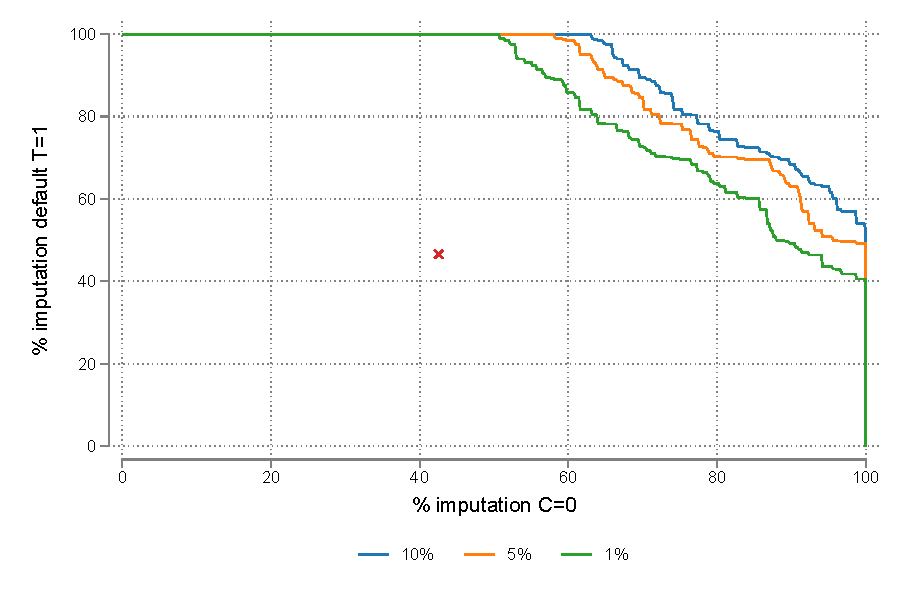
\includegraphics[width=\textwidth]{Figuras/frontera_sig_apr.pdf}
%    %  \end{subfigure}     
%    %  \begin{subfigure}{0.49\textwidth}
%    % \caption{Significance area for Default }
%         \centering
%         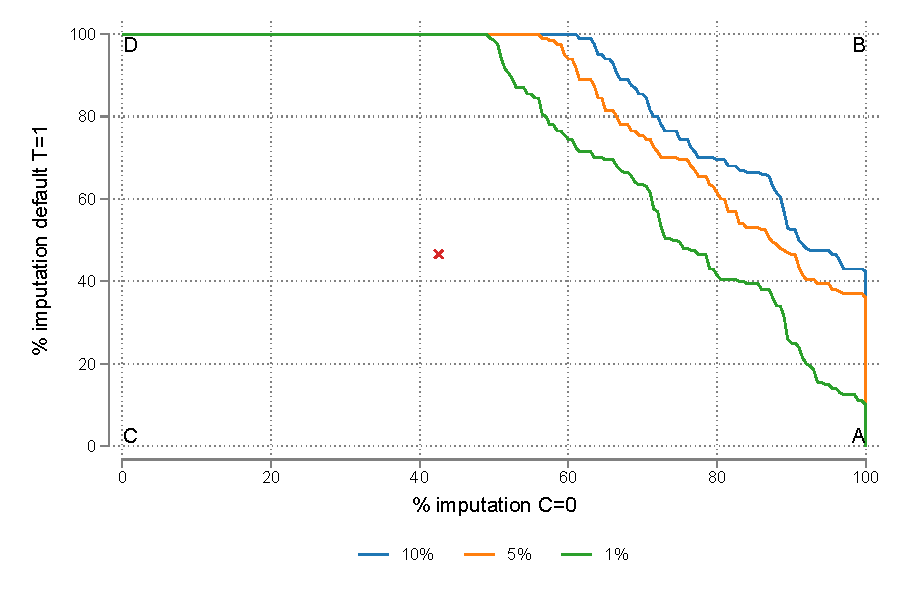
\includegraphics[width=0.5\textwidth]{Figuras/frontera_sig_def_imp.pdf}
%     % \end{subfigure} 
%     \end{center}
%  \caption{Interpolation on bounding censoring for Default. This figure aims to answer the following question: For how many loans in the control arm can we impute recovery, and for how many in the treatment arm can we impute default and still have significance?
%      This figure shows exactly the boundary separating significance when we vary the percentage of imputed censored loans with recovery and default respectively for control and treatment. Each corner in the square will correspond to one of the panels from the Table \ref{bounding_censoring}. For instance, the origin is the best-case scenario (Panel C) and the point (100,100) (Panel B) is the worst-case scenario. Thus we can think of this graph as an `interpolation' from the four extreme cases. The `x' indicates the proportions imputed by the lasso logit model, and the different lines correspond to setting different significance levels. We do not include the plot for APR nor financial cost, since for any imputation we still have significant results.}
%  \label{interpolation_censoring_imp}
%      %\textit{Do file: }  \texttt{interpolation_censoring_imp.do}
% \end{figure}





\begin{figure}[H]
\caption{Survival graph.}
    \begin{center}
   \begin{subfigure}{0.49\textwidth}
   \caption{Ended contract}
        \centering
        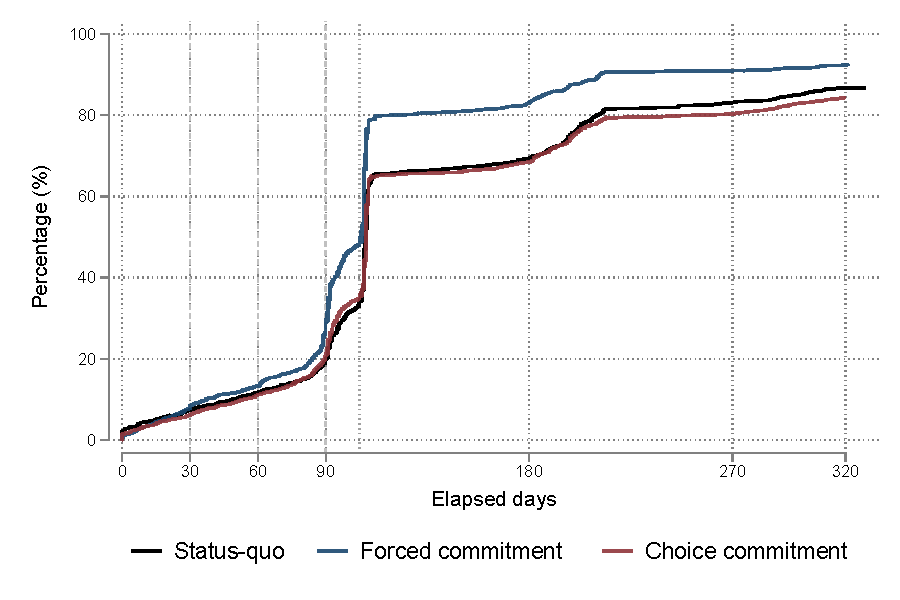
\includegraphics[width=\textwidth]{Figuras/survival_graph_ended.pdf}
    \end{subfigure} 
   \begin{subfigure}{0.49\textwidth}
   \caption{Recovery}
        \centering
        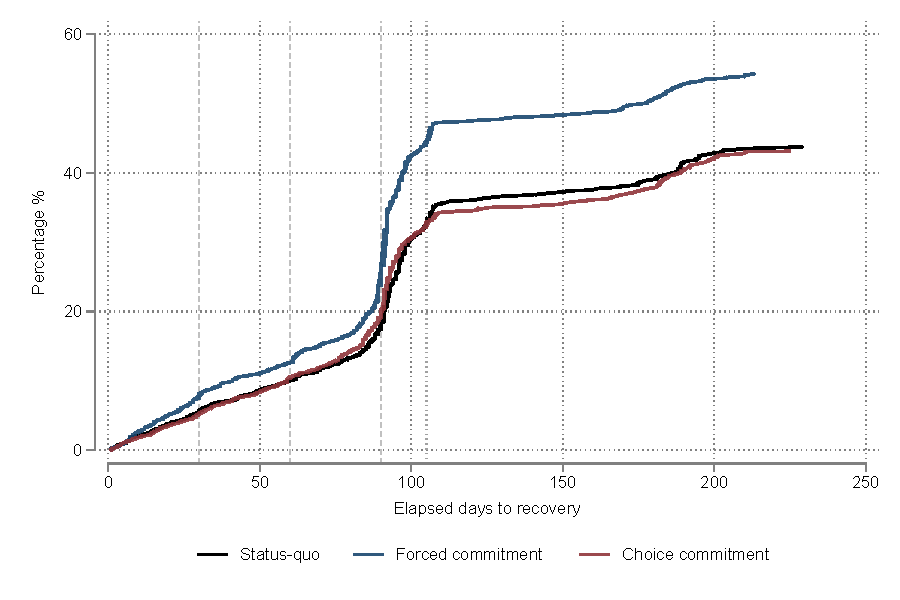
\includegraphics[width=\textwidth]{Figuras/survival_graph_unpledge.pdf}
    \end{subfigure}     
    \end{center}
      \footnotesize{This Figure shows the CDF of loan completion either default or recovery in Panel (a), or loan recovery in Panel (b), by the number of days since first pawn.}
      \label{survival_graph}
     %\textit{Do file: }  \texttt{survival\_graph.do}
\end{figure}

% \begin{figure}[H]
%     \begin{center}
%    \begin{subfigure}{0.49\textwidth}
%         \caption{Unconditional}
%         \centering
%         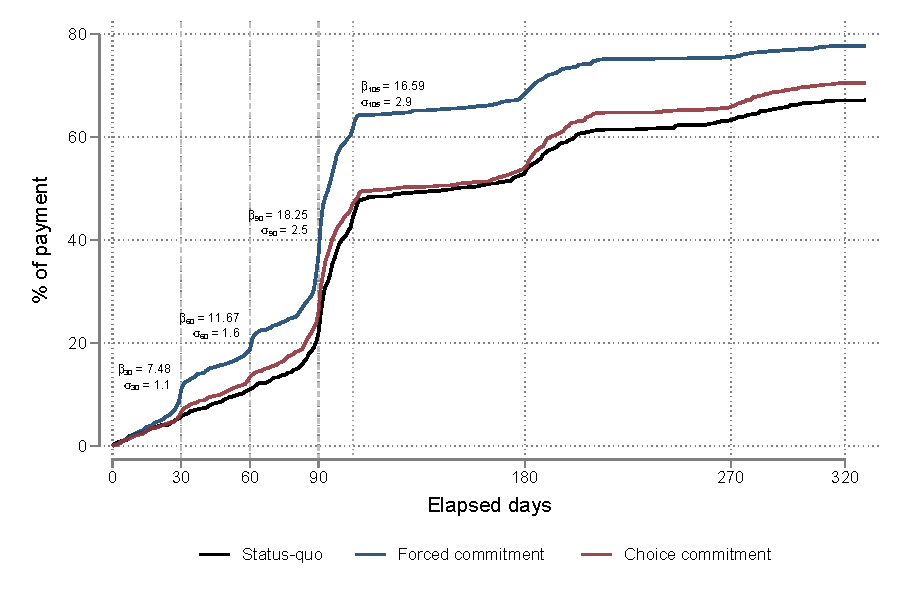
\includegraphics[width=\textwidth]{Figuras/cumulative_porc_pay_time.pdf}
%     \end{subfigure} 
%    \begin{subfigure}{0.49\textwidth}
%         \caption{Conditional on default}
%         \centering
%         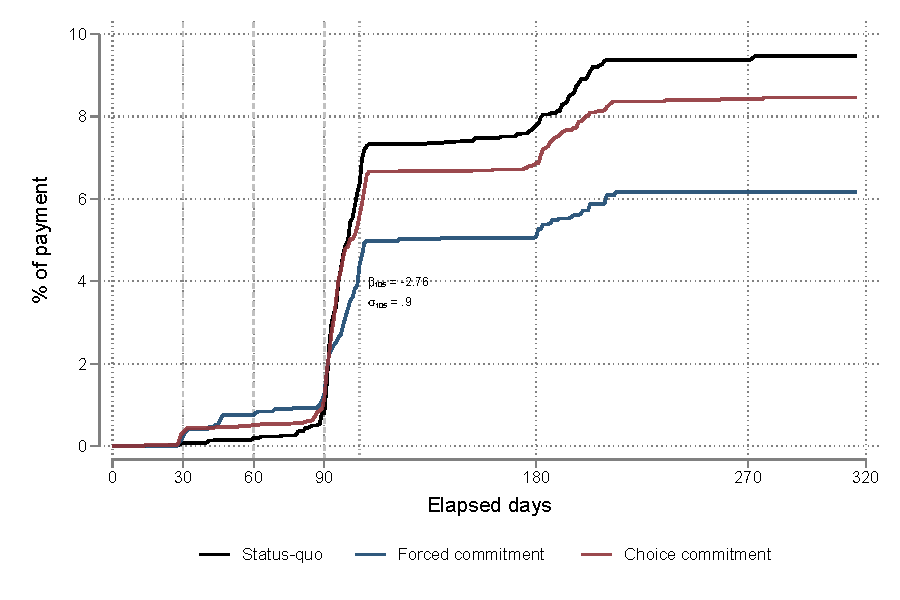
\includegraphics[width=\textwidth]{Figuras/cumulative_porc_pay_time_default.pdf}
%     \end{subfigure}     
%     \end{center}
%     \caption{\% of payment over time. This Figure shows the accumulated percentage of recovery in time by treatment arm. }
%     \label{porc_payment_over_time}
%      %\textit{Do file: }  \texttt{cumulative\_porc\_pay\_time.do}
% \end{figure}




\subsection{Robustness accounting for other costs}

\begin{table}[!h]
\caption{Effects on more comprehensive cost measures}
\label{table_robustness_fc}
\begin{center}
\resizebox{0.95\textwidth}{!}{
\footnotesize{% Table generated by Excel2LaTeX from sheet 'fc_robustness'
\begin{tabular}{lccccc}
\toprule
      & FC    & FC (subj.value) & FC +  tc & FC - interest & FC (subj.value) + tc - int \\
\midrule
      & (1)   & (2)   & (3)   & (4)   & (5) \\
\midrule
\midrule
Forced commitment & -204.0*** & -299.9*** & -207.7*** & -98.5*** & -146.3** \\
      & (48.1) & (83.3) & (49.0) & (36.7) & (72.8) \\
Choice comitment & -38.9 & -56.4 & -32.6 & -30.7 & -25.3 \\
      & (49.8) & (83.5) & (50.9) & (39.2) & (74.4) \\
      &       &       &       &       &  \\
\midrule
Observations & 6304  & 6304  & 6304  & 6304  & 6304 \\
R-squared & 0.013 & 0.009 & 0.014 & 0.005 & 0.006 \\
Control Mean & 942.4 & 1389.9 & 1026.1 & 480.7 & 927.7 \\
\midrule
\midrule
      &       &       &       &       &  \\
\midrule
      & APR   & APR (subj.value) & APR +  tc & APR - interest & APR (subj.value) + tc - int \\
\midrule
      & (6)   & (7)   & (8)   & (9)   & (10) \\
\midrule
\midrule
Forced commitment & -0.11*** & -0.22*** & -0.13*** & -0.062*** & -0.097** \\
      & (0.019) & (0.051) & (0.028) & (0.019) & (0.044) \\
Choice comitment & -0.0086 & -0.053 & -0.0035 & -0.031* & -0.043 \\
      & (0.019) & (0.045) & (0.028) & (0.018) & (0.040) \\
      &       &       &       &       &  \\
\midrule
Observations & 6304  & 6304  & 6304  & 6304  & 6304 \\
R-squared & 0.031 & 0.011 & 0.027 & 0.008 & 0.007 \\
Control Mean & 0.57  & 1.12  & 0.72  & 0.31  & 0.84 \\
\bottomrule
\bottomrule
\end{tabular}%
}
}
\end{center}
 \footnotesize{ This table augments the measure of financial cost presented in Table \ref{main_impact_table} with measures of transaction costs, subjective costs, and adjustments for liquidity costs. Panel A reports financial cost in pesos, while Panel B shows APR. Columns (1) and (6) replicate our previous results for comparability. Columns (2) and (7) of Table \ref{table_robustness_fc} use the subjective value of the pawn reported by the borrower rather than its appraised value. Columns (3) and (8) adjust for self-reported transport costs per visit plus an entire day's wage, both multiplied by the number of visits that each individual made.\footnote{For clients who did not complete the individual survey, we adjust using the mean self-reported transport cost among respondents of the respective branch.} Columns (4) and (9) adjust to consider the liquidity cost. Finally, columns (5) and (10) include all three changes together. The main takeaway from the table is that results are quite robust to including a much expanded measure of costs. Each regression includes branch and day-of-week FE. Standard errors are clustered at the branch-day level.}
%\textit{Do file: } \texttt{fc\_robustness.do}
\end{table}

\newpage 

\normalsize

%Really force it to normal size and linespread
\normalsize


\subsection{Repawning}

We now estimate equation \ref{basic_reg} with Different dependent variables.  In column 1, the dependent variable indicates, for each borrower in the experiment, whether he/she pawned again after the first loan in the
experiment (up to the end period of our data set 338 days after the experiment began). The result is that the likelihood of repeat business increases by 6.7\%.  While this appears to be \emph{prima facie} evidence of greater satisfaction among borrowers in the forced arm, the interpretation is complicated by the fact that monthly payments may themselves trigger more borrowing to pay them. Note that from the lender's perspective, why repeat pawning happens may not be as important as the fact that it happens. Illiquidity does not seem to drive this result, given that the effect on re-pawning comes after 90 days (during the period of contract demanded payments) and not before  (see columns 2 and 3). Column 4 only considers new loans that use different collateral from that of the initial one. We do this to foreclose the explanation that those in the Forced arm, being more liquidity-constrained, return to pawn a second pawn to be able to pay the monthly payments of their first loan. However, we cannot reject a zero effect on pawning a different collateral. Column 5 focuses on the (endogenous) subsample of those recovering their pawn in both arms of the experiment. This means that \textit{both} arms have recovered their pawn and could re-pawn if they so wish, and also that the liquidity demands from the monthly contract are \textit{no longer} there as the contract has been closed.  We find that the difference between the Forcing contract and the status quo is even larger in this subsample, with the former having 11pp higher likelihood of being a repeat client during our sample period.

\begin{table}[!h]
\caption{Effects on Repeat Pawning}
\label{repeat_loans}
\begin{center}
\footnotesize{% Table generated by Excel2LaTeX from sheet 'repeat_loans'
\begin{tabular}{lcccccccc}
\toprule
      & \multicolumn{6}{c}{Ever pawns again (ITT)}    &       &  \\
\cmidrule{2-7}      &       & Cond. on rec & Cond. on default & Different collateral & After 90 days & Within 90 days &       & Days from 1st loan  \\
\midrule
\midrule
      & (1)   & (2)   & (3)   & (4)   & (5)   & (6)   &       & (7) \\
\midrule
\midrule
Forced commitment & 0.067* & 0.10** & -0.0046 & 0.036 & 0.037*** & 0.032 &       & 7.72** \\
      & (0.035) & (0.047) & (0.035) & (0.030) & (0.013) & (0.027) &       & (3.07) \\
Choice commitment & 0.040 & 0.051 & 0.026 & 0.027 & 0.0098 & 0.030 &       & 1.72 \\
      & (0.031) & (0.042) & (0.034) & (0.027) & (0.0087) & (0.026) &       & (2.59) \\
      &       &       &       &       &       &       &       &  \\
\midrule
Observations & 4441  & 2168  & 2273  & 4441  & 4441  & 4441  &       & 1577 \\
R-squared & 0.003 & 0.007 & 0.001 & 0.001 & 0.006 & 0.001 &       & 0.011 \\
Control Mean & 0.32  & 0.36  & 0.29  & 0.28  & 0.020 & 0.30  &       & 32.9 \\
\bottomrule
\bottomrule
\end{tabular}%
}
\end{center}
 \footnotesize{This table estimates the specification of equation \ref{basic_reg} but at the level of the borrower (not the loan). Each column represents a regression with a different outcome variable. In column 1, the dependent variable indicates, for each borrower in the experiment, whether he/she pawned again after the first loan in the experiment (up to the end period of our data set 338 days after the experiment began). Column 2 is analogous, but only pawning after 90 days of the first loan is considered. Column 3 instead considers pawning before 90 days. Column 4 is analogous to column 1 but focuses on the pawning of a gold piece that is different from the one in the first experimental loan. Column 5 is analogous to column 1, but conditioning on the sample that recovered the first loan. 
Standard errors are clustered at the branch-day level.}
%\textit{Do file: } \texttt{repeat\_loans.do}
\end{table}



\begin{table}[!h]
\caption{Lender's Profit}
\label{lenders_profit}
\begin{center}
 \footnotesize{% Table generated by Excel2LaTeX from sheet 'lenders_profit'
\begin{tabular}{lcccc}
\toprule
      & \multicolumn{4}{c}{Lender's Profit} \\
\midrule
      & Empirical  &       & \multicolumn{2}{c}{Back-of-the-envelope} \\
\cmidrule{2-2}\cmidrule{4-5}      & (1)   &       & (2)   & (3) \\
\midrule
\midrule
Forced Commitmment & -259.5** &       & -146.3** & -196.1*** \\
      & (131.2) &       & (61.4) & (59.1) \\
Choice Commitment & 44.1  &       & 67.8  & 55.4 \\
      & (152.2) &       & (74.6) & (76.1) \\
      &       &       &       &  \\
\midrule
Observations & 4441  &       & 6304  & 6304 \\
R-squared & 0.002 &       & -     & - \\
Control Mean & 1792.1 &       & 1372.31 & 1531.31 \\
\bottomrule
\bottomrule
\end{tabular}%
}
\end{center}
 \footnotesize{ The dependent variable in column (1) is the profit formula in equation (\ref{profit_function}). For columns (2)-(3) we compute average profit for borrower in arm $j$ according to (\ref{profit_function}). We then extrapolate the flow of payments over several periods depending on their repeat pawning behavior. In column (2) the flow of profits is given by
 \[\sum_{T=0}^{\infty}\text{Profit}_j\times\Pr(\text{Pawn}_j)^T\]
 assuming independence of repeat pawning across periods. In column (3) the stream of profits is given by
 \[\text{Profit}_j + \text{Profit}_j\times \Pr(\text{Pawn}_j) +\text{Profit}_j\times\Pr(\text{Pawn}_j) \]
 assuming that once learning (and hence repeat pawning behavior) occurs the borrower keeps coming back (we only keep 2 further periods for the exercise).
 For columns(2)-(3) we clustered-bootstrapped the standard error. All Standard errors are clustered at the branch-day level.}
%\textit{Do file: } \texttt{lenders\_profit.do}
\end{table}

\newpage


\section{ Alternative explanations}
\subsection{Learning}


Table \ref{learning_table} presents information about borrowers' \emph{future} pawning behavior as a function of treatment assignment. Column (1) considers the 228 clients who returned only a second time to pawn again at a day/branch that was randomly assigned to the choice arm. Each of the two rows in this column presents a difference of mean commitment take-up rates, and associated standard error. The first row compares those who were \emph{initially} assigned to forced commitment against those where were assigned to control; the second row compares those who were initially assigned to the choice commitment arm to those who were assigned to the other two arms. In each case, there is no statistically discernible difference in the rates of commitment take-up. Granted, this is a selected sample because the decision to pawn again is potentially endogenous to the initial treatment allocation. For this reason, Column (2) considers the full sample of 4441 borrowers by re-defining the outcome variable to be an indicator for returning to pawn again at a branch/day when commitment was offered \emph{and} choosing commitment. This composite outcome variable is not subject to the sample selection problem (although it is directly driven by the decision to repeat borrow). The comparison in the two rows remains the same: forced commitment versus control in row one and choice commitment versus forced arms in row two. Again, there is no statistically discernible difference in commitment take-up rates in either row. While these exercises cannot completely exclude the possibility that learning plays a role, they provide no indication that the lack of voluntary compliance is simply a matter of inexperience with commitment.



\begin{table}[H]
        \caption{Effect of Prior Assignment on Subsequent Choice}
    \label{learning_table}
\begin{center}
\footnotesize{% Table generated by Excel2LaTeX from sheet 'learning_exp'
\begin{tabular}{lccc|ccc}
\toprule
      & \multicolumn{3}{c|}{Choose Fee} & \multicolumn{3}{c}{Choose Promise} \\
\midrule
      & (1)   & (2)   & (3)   & (4)   & (5)   & (6) \\
\midrule
\midrule
Fee-forcing (FF) & 0.078 & 0.016 & 0.090 & 0.094 & -0.029 & 0.17 \\
      & (0.076) & (0.087) & (0.12) & (0.11) & (0.15) & (0.16) \\
Fee-promise (FP) & 0.085 & 0.033 & 0.19  & -0.030 & -0.082 & -0.14 \\
      & (0.11) & (0.034) & (0.17) & (0.18) & (0.28) & (0.20) \\
Choice/SQ (CSQ) & 0.069 & 0.10  & 0.14  & 0.085 & 0.12  & 0.17 \\
      & (0.063) & (0.063) & (0.13) & (0.071) & (0.11) & (0.11) \\
Choice/Fee (CF) & -0.049 & -0.094 & -0.017 & -0.20 & 0.26  & -0.28 \\
      & (0.10) & (0.10) & (0.14) & (0.16) & (0.29) & (0.22) \\
Decision epoch 2 (D2) &       & -0.16 &       &       & -0.21 &  \\
      &       & (0.16) &       &       & (0.22) &  \\
Decision epoch 3 D(3) &       & 0.037 &       &       & 0.027 &  \\
      &       & (0.034) &       &       & (0.15) &  \\
FF\#D2 &       & 0.17  &       &       & 0.46  &  \\
      &       & (0.20) &       &       & (0.28) &  \\
FF\#D3 &       & -0.017 &       &       & -0.14 &  \\
      &       & (0.081) &       &       & (0.27) &  \\
FP\#D2 &       & 0.49  &       &       & 0.30  &  \\
      &       & (0.29) &       &       & (0.34) &  \\
FP\#D3 &       & -0.30 &       &       & -0.016 &  \\
      &       & (0.27) &       &       & (0.39) &  \\
CSQ\#D2 &       & 0.096 &       &       & 0.12  &  \\
      &       & (0.16) &       &       & (0.24) &  \\
CSQ\#D3 &       & -0.16 &       &       & -0.044 &  \\
      &       & (0.084) &       &       & (0.18) &  \\
CF\#D2 &       & 0.062 &       &       & -0.38 &  \\
      &       & (0.29) &       &       & (0.29) &  \\
CF\#D3 &       & 0.071 &       &       & -0.39 &  \\
      &       & (0.16) &       &       & (0.36) &  \\
Default (Def) &       &       & 0.15  &       &       & 0.12 \\
      &       &       & (0.13) &       &       & (0.14) \\
FF\#Def &       &       & 0.19  &       &       & -0.17 \\
      &       &       & (0.25) &       &       & (0.20) \\
FP\#Def &       &       & -0.23 &       &       & 0.13 \\
      &       &       & (0.18) &       &       & (0.24) \\
CSQ\#Def &       &       & -0.13 &       &       & -0.17 \\
      &       &       & (0.13) &       &       & (0.17) \\
CF\#Def &       &       & 0.031 &       &       & 0.11 \\
      &       &       & (0.14) &       &       & (0.30) \\
      &       &       &       &       &       &  \\
\midrule
Observations & 150   & 150   & 150   & 152   & 152   & 152 \\
R-sq  & 0.720 & 0.768 & 0.763 & 0.640 & 0.681 & 0.651 \\
DepVarMean & \multicolumn{3}{c|}{0.053} & \multicolumn{3}{c}{0.20} \\
Individual FE & \checkmark & \checkmark & \checkmark & \checkmark & \checkmark & \checkmark \\
\bottomrule
\bottomrule
\end{tabular}%
}
\end{center}
 \footnotesize{Column (1) reports results for the 228 borrowers who returned to pawn again at a day/branch that was randomly assigned to the choice arm, enabling us to observe whether they chose commitment or the status quo contract.
Each row presents a difference in mean commitment take-up rates and associated standard errors.
The first row (ATE) compares borrowers who were initially assigned to forced commitment against those were assigned to the control condition.
The second row (ITT) compares borrowers who were initially assigned to the choice commitment condition to those who were not.
Whereas column (1) conditions on the (endogenously) selected sample of borrowers who return to pawn again, column (2) considers the full sample by re-defining the ``outcome'' to be an indicator for whether a borrower pawned again on a day when choice was offered \emph{and} chose commitment.}

%This table explores learning by focusing on a subsample of borrowers in the experiment and observing their subsequent behavior. Column 1 conditions the sample on borrowers who (a) pawned during the experiment a subsequent time after being assigned to control, forced commitment or choice (the regressors), and (b) when pawning again they went to a branch day when (randomly) choice was available, thus enabling us to observe if they chose the commitment contract or the status quo.  in this sample it estimates a linear probability model where the dependent variable is equal to one if the borrower chose the commitment contract in that subsequent `choice' occasion and zero otherwise. The regressors are indicators for the treatment arms in their first pawn in the experiment. Column 1 conditions the sample on the (endogenous) event of pawning again. Column 2 does not condition the sample, but instead defined the dependent variable as equal to one \hl{if the borrower pawned subsequently and choice was available that day and chose commitment, and zero otherwise.}

\end{table}
\normalsize
%Really force it to normal size and linespread
\normalsize


\subsection{Discount rates}


\begin{figure}[!h]
  \caption{Financial benefit TUT effect for different discount rates.}
    \begin{center}
        \centering
        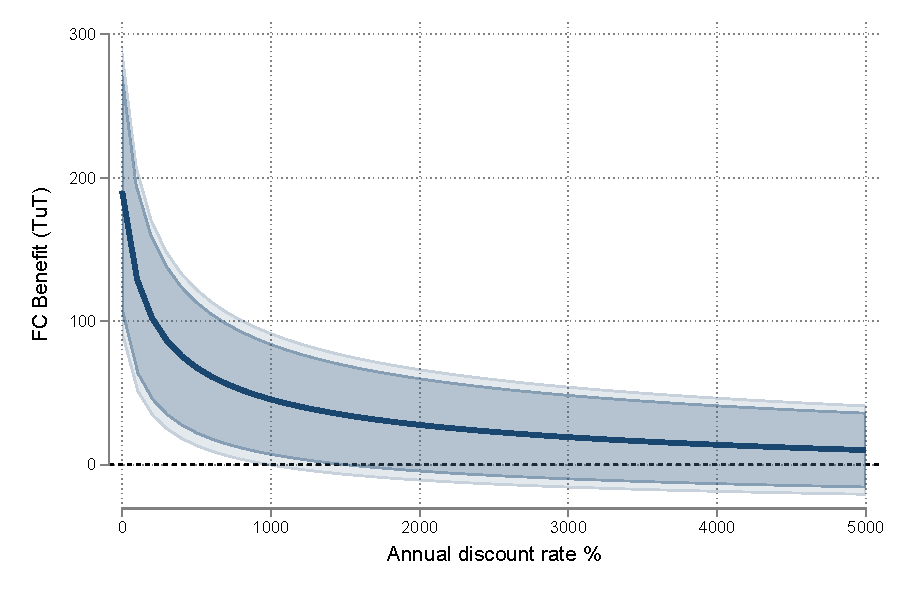
\includegraphics[width=0.65\textwidth]{Figuras/discount_effect_tut.pdf}
    \end{center}
       \footnotesize{This Figure re-estimates the treatment on the untreated (TUT) effect from Table \ref{tot_tut}, introducing a daily discount factor in the definition of financial benefit.  At a given annual discount rate in percentage points (x-axis) the solid line gives the adjusted TUT and the shaded regions 90\% \& 95\% confidence bands. A discount factor of one corresponds to the estimate from Table \ref{tot_tut}. As seen from the figure, borrowers would need to face unrealistically large discount rates to reverse our headline result of a large, positive, and statistically significant TUT effect.}
        \label{fc_discount_rates}
     %It estimates the effect of the treatment arms  for different discount factors, where a discount factor of 1 corresponds exactly to the estimate of column 1 of Table \ref{main_impact_table}. Because the commitment contract induces earlier payments, this adjusted financial cost will be higher, and thus financial savings will be lower. This figure shows the range of estimated effects and their confidence intervals, where the discount rate used is ploted in the x-axis annualized.    %\textit{Do file: }  \texttt{discounted\_noeffect.do}
\end{figure}

\normalsize
%Really force it to normal size and linespread
\normalsize


\subsection{Present Bias}\label{App_presentbias}

\noindent \textbf{Present bias.} If the benefits of commitment among non-choosers cannot be explained by standard models of rational choice, the canonical behavioral story would center on time inconsistency.  While commitment is useful to anyone with hyperbolic time preferences, only those who are sophisticated--i.e.\ aware that they are hyperbolic discounters--will demand it.  A large share of ``na\"ive'' hyperbolics in the population--borrowers who are unaware that they are hyperbolic discounters--could therefore drive a large and positive $\text{TUT}$.  Our baseline survey included standard questions about discount rates between today and a month in the future versus discount rates between three and four months in the future.
This allows us to classify borrowers who display more impatience over immediate delays as present biased. This measure of financial hyperbolicity is widely used in survey research, although it is not without problems.\footnote{Our measure is dichotomous, and it is not incentivized. Recent empirical work has shown the superiority of more elaborate measures such as ``convex time budgets'' \citep{andreoni2015measuring} while questioning the interpretation of measures of hyperbolicity that are not based on consumption \citep{andreoni2012estimating, cohen2020measuring}, suggesting that real effort tasks provide a better measure \citep{augenblick2015working}.  Given that we had only a few minutes to interview real pawnshop clients prior to a commercial transaction, our simple measure was a necessary compromise.}   

If we could perfectly measure present bias and sophistication, we could divide the sample into three groups: sophisticated hyperbolics (who chose commitment), time-consistent non-choosers (for whom forcing will not be effective), and na\"{i}ve hyperbolic non-choosers (who will benefit from forced commitment). %If present bias fully explains the low take-up rate of voluntary commitment, we should find that the TUT for present-biased borrowers  is positive while the TUT for all other borrowers is not.
If present bias fully explains the low take-up rate of voluntary commitment, we should find that the TUT for present-biased borrowers is positive. This is because among the group of non-takers, a comparison of present-biased borrowers against everyone else is a comparison of na\"{i}ve hyperbolics against time-consistent non-choosers. 

The left panel of Figure \ref{tut_beh_partition} carries out a feasible version of this exercise using our survey measure of present bias.
The overall TUT estimate along with a 95\% confidence interval is given in blue.\footnote{For all borrowers who answered our present-bias survey questions.}
The corresponding TUT estimate and confidence interval for present-biased borrowers identified with the survey question is given in green; results for all other borrowers are shown in red.
The overall TUT is a weighted average of the impact in these two sub-groups.  The TUT among the present biased is insignificant and less than half the size of the strongly significant TUT among those who are \textit{not} present biased. Therefore, taking our survey measure of hyperbolicity at face value, we find no indication that present-bias explains our positive estimated TUT. 



\begin{figure}
\caption{Heterogeneity of the TUT by behavioral variables.}
    \begin{center}
        \centering
        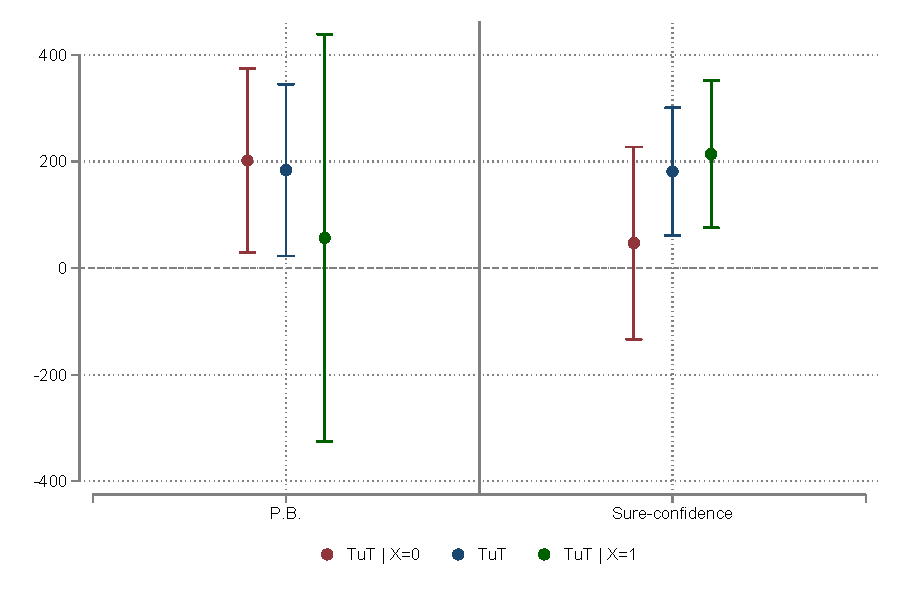
\includegraphics[width=0.65\textwidth]{Figuras/tut_beh_partition.pdf} 
    \end{center}  
 \footnotesize{Each panel in this figure shows how the estimated treatment on the untreated (TUT) effect varies with a binary survey variable $X_i$. In the left panel (P.B.), $X_i = 1$ if borrower $i$ is ``present-biased'' based on her responses to the time preference questions from our survey. In the right panel (Sure-confidence) $X_i = 1$ if  borrower $i$ reported that she was certain to recover her pawn, zero otherwise. }
    \label{tut_beh_partition}
      %\footnotesize{ \textit{Do file: }  \texttt{partition_tut.do}

\end{figure}
\subsection{Sure Confidence} \label{App_sureconfidence}

\begin{figure}[H]
\caption{Determinants sure confidence.}
    \begin{center}
    \begin{subfigure}{0.60\textwidth}
        \centering
        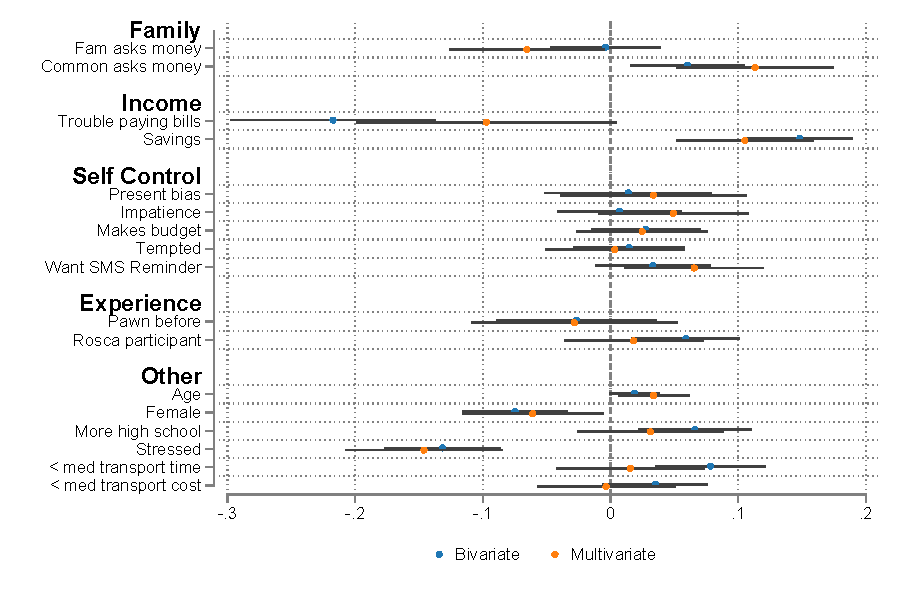
\includegraphics[width=\textwidth]{Figuras/determinants_confidence_100.pdf}
    \end{subfigure}
    \end{center}
     \footnotesize{The above figure shows the determinants in a bivariate and multivariate OLS regression of sure confidence among the non-choosers. Sure confidence is a binary variable defined to be one when people report a 100\% probability of recovery.}
    \label{determinants_sure}
%\textit{Do file: } \texttt{determinants_sure_confidence.do}       
\end{figure}


\newpage


%\section{ Heterogeneity and Bounds}
\section{Bounds, FOSD and Rank Invariance} \label{bounds_FOSD}

%\subsection{Testing for heterogeneity}
%\label{append:chernozhukov}
%If the treatment effects $Y_{i1} - Y_{i0}$ are constant across $i$, then we must have
%\[
%\text{ATE}(X_i) \equiv \mathbbm{E}[Y_{i1} - Y_{i0} |X_i] = \mathbbm{E}[Y_{i1} - Y_{i0}] \equiv \text{ATE}
%\]
%for any covariates $X_i$ that vary across $i$. If, on the other hand, $\text{ATE}(X_i)$ can be predicted using some scalar function $\tau(\cdot)$ of $X_i$, then the average treatment effect function is not constant so there must be treatment effect heterogeneity. 
%
%We operationalize this idea using a two-step approach proposed by \cite{chernozhukov2018generic}.  We begin by randomly dividing the participants in the forced arms of the experiment ($Z_i \neq 2$) into two groups: a training set and a test set.
%These sets are constructed to ensure that all observations from a given branch-day cluster are allocated to the same set.
%This avoids inferential problems that could arise from correlated unobservables within clusters.
%In the first step, we apply the generalized random forest approach of \cite{atheygrf} to the training set to estimate two proxy predictors: $\psi(\cdot|\text{Training})$ approximates the untreated potential outcome function, $\mathbbm{E}[Y_{i0}|X_i] = \mathbbm{E}[Y_i|Z_i=0,X_i]$, while  $\tau(\cdot|\text{Training})$, approximates the ATE function
%\[
%\text{ATE}(X_i) = \mathbbm{E}[Y_i|Z_i=1,X_i] - \mathbbm{E}[Y_i|Z_i=0, X_i].
%\]
%The proxy predictors need not be unbiased or even consistent estimators of the functions they aim to approximate: the goal of this exercise is merely to find a scalar function of $X_i$ that \emph{accurately predicts} $\text{ATE}(X_i)$.
%In the second step we fit a linear regression model to data from the training set using regressors constructed from the proxy functions $\psi(\cdot|\text{Training})$ and $\tau(\cdot|\text{Training})$ constructed in the first step. In particular, we estimate 
%\begin{equation}
%Y_i = \alpha_0 + \alpha_1 \psi_i + \beta_1 (Z_i - \mathbbm{E}[Z_i]) + \beta_2 (Z_i - \mathbbm{E}[Z_i])(\tau_i - \mathbbm{E}[\tau_i]) + \epsilon_i
%\label{eq:chernreg}
%\end{equation}
%where $\psi_i \equiv \psi(X_i|\text{Training})$ and $\tau_i \equiv \tau(X_i|\text{Training})$.\footnote{This is a slightly simpler regression than the one proposed in equation (3.1) of \cite{chernozhukov2018generic}, which involves propensity score weights. Because the random assignment of $Z$ in our experiment does \emph{not} condition on $X$, the propensity score weights in our case are constant over $X$ and hence drop out.} As shown by \cite{chernozhukov2018generic}, the coefficients $\beta_1$ and $\beta_2$ from \eqref{eq:chernreg} identify the \emph{best linear predictor} of the conditional ATE based on $\tau(\cdot|\text{Training})$, namely
%\[
%\beta_1 = \mathbbm{E}[\text{ATE}(X_i)] = \text{ATE}, \quad
%\beta_2 = \frac{\text{Cov}[\text{ATE}(X_i), \tau_i]}{\text{Var}(\tau_i)}.
%\]
%If treatment effects are homogeneous we must have $\beta_2 = 0$. Rejecting this hypothesis establishes that $\tau_i$ predicts $\text{ATE}(X_i)$ and hence that $\Delta_i$ varies. 
%Since $\tau_i$ and $\psi_i$ do not depend on the test set, inference for the regression in \eqref{eq:chernreg} is straightforward conditional on the Training/Test split.  
%Our estimate for $\beta_2$ is 2.56 with a one-sided heteroskedasticity-robust (HC3) standard error of 0.43.
%Thus we easily reject the null hypothesis of homogeneous treatment effects.

%\todo[inline]{Discuss the results here.}

%\todo[inline]{Issac: re-run this exercise with removing the propensity score weights $p(Z)$. Presumably it shouldn't change anything, but it's simpler to explain what we do and probably less noisy}

%\begin{table}[H]
%\begin{center}
%\footnotesize{% Table generated by Excel2LaTeX from sheet 'test_calibration_2'
\begin{tabular}{rccccc}
\toprule
      & \multicolumn{5}{c}{Test Calibration} \\
\midrule
      & \multicolumn{2}{c}{With PS} &       & \multicolumn{2}{c}{Without PS} \\
\cmidrule{2-3}\cmidrule{5-6}      & \multicolumn{2}{c}{APR} &       & \multicolumn{2}{c}{APR} \\
\cmidrule{2-3}\cmidrule{5-6}      & BVC   & BVC + survey variables &       & BVC   & BVC + survey variables \\
\midrule
      & (1)   & (2)   &       & (3)   & (4) \\
\midrule
\midrule
\multicolumn{1}{l}{Mean Forest Prediction} & 0.9797 & 0.9983 &       & 0.8302 & 0.8816 \\
      & (0.1335) & (0.1165) &       & (0.1198) & (0.1034) \\
\multicolumn{1}{l}{Differential Forest Prediction} & 0.9486 & 1.3224 &       & 0.8107 & 1.2027 \\
      & (0.1270) & (0.2073) &       & (0.1163) & (0.1861) \\
\bottomrule
\bottomrule
\end{tabular}%
}
%\end{center}
%\end{table}

%\todo[inline]{Some Questions for Issac: (1) How are we carrying out the sample splitting? If we cluster standard errors at the branch-day level, we should take this into account when we split. (2) How are you carrying out inference for $\beta_2$? Chernozhukov et al discuss two approaches: ``conditional'' and ``variational.'' The former is simpler as it conditions on the training/test split. The latter is a bit more involved, since one accounts for uncertainty arising from different splits. (3) What are the details of the random forest procedure employed here? (Tuning parameters choice, etc.) We should put them into the appendix.}

%\newpage

\begin{figure}[!h]
   \caption{Fan \& Park bounds for benefit in APR\%.}
    \begin{center}
    \begin{subfigure}{0.65\textwidth}
        \caption{APR Bounds}
        \centering
        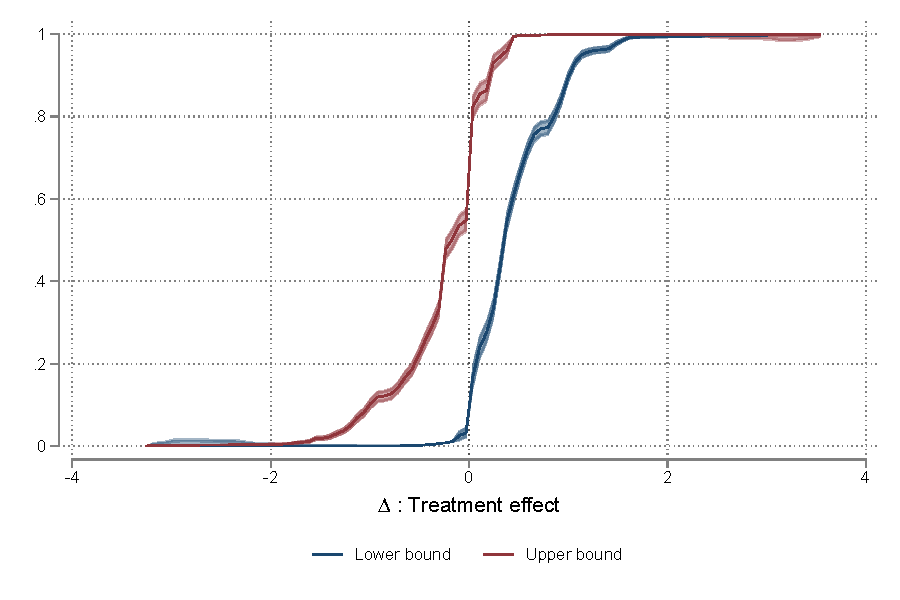
\includegraphics[width=\textwidth]{Figuras/fan_park_bounds_apr.pdf}
    \end{subfigure}
    \end{center}
          \footnotesize{This figure depicts the \cite{fan2010sharp} bounds on the distribution $F_\Delta$ of individual treatment effects $\Delta \equiv (Y_1 - Y_0)$, described in Section \ref{sec:bounds}, for the APR outcome.
    The dark red curve and light red shaded region give the estimated upper bound function $\overline{F}$ for $F_\Delta$ and associated (pointwise) 95\% confidence interval. 
    The dark blue curve and light blue shaded region give the estimated lower bound function $\underline{F}$ for $F_\Delta$ and associated (pointwise) 95\% confidence interval.
    Confidence intervals are computed using the asymptotic distribution for the bounds.  Evaluating the bounds at $\delta = 0$, we see that between 23\% and 97\% of borrowers have a positive individual treatment effect.}
     \label{fan_park_bounds}
%\textit{Do file: } \texttt{fan\_park\_bnds.do}       
\end{figure}

\begin{figure}[!h]
\caption{Distribution of treatment effects under rank invariance.}        
    \begin{center}
       \begin{subfigure}{0.49\textwidth}
        \caption{APR benefit}
        \centering
        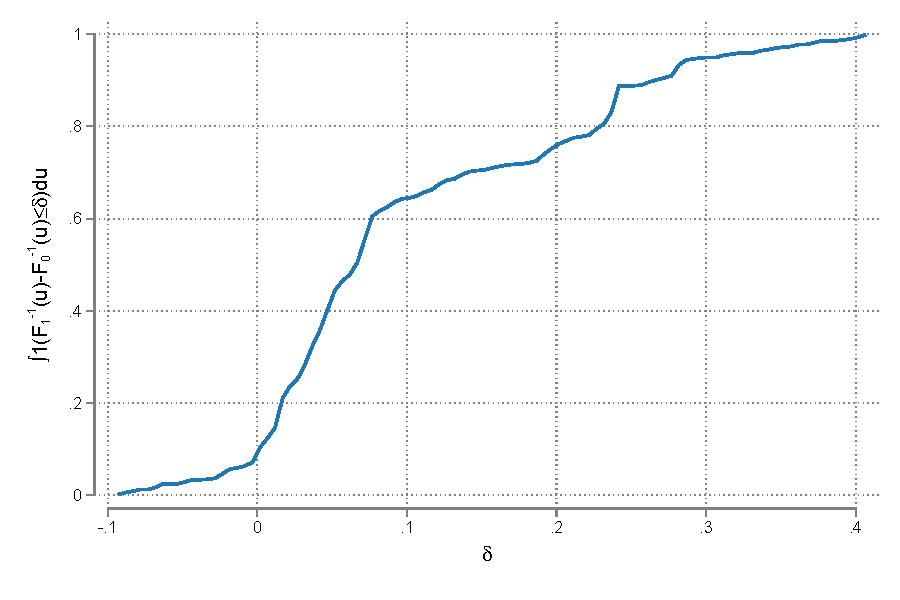
\includegraphics[width=\textwidth]{Figuras/te_rankinvariance_apr.pdf}
    \end{subfigure} 
   \begin{subfigure}{0.49\textwidth}
        \caption{Financial benefit}
        \centering
        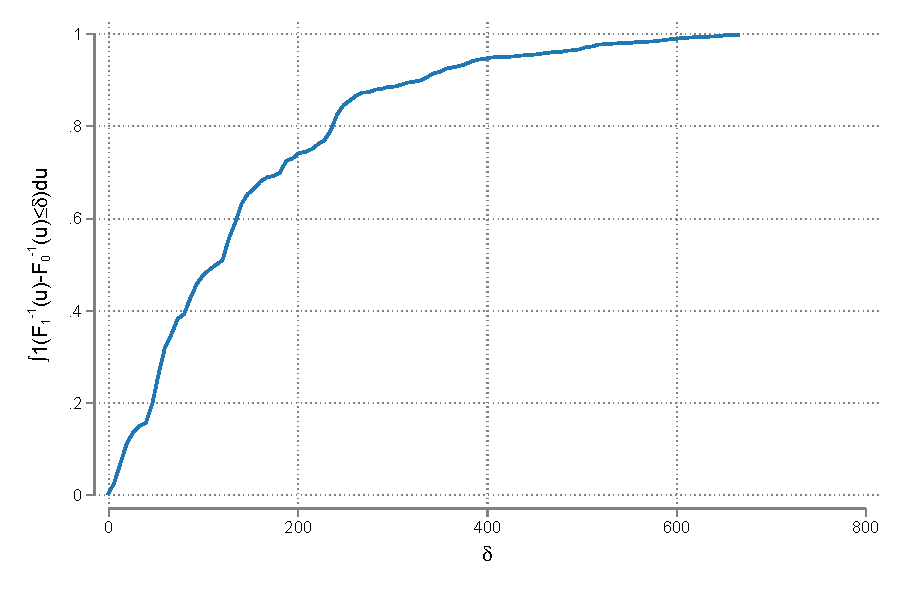
\includegraphics[width=\textwidth]{Figuras/te_rankinvariance_fc_admin.pdf}
    \end{subfigure} 
    \end{center}
    \footnotesize{This figure shows the CDF of individual treatment effects under the assumption of rank invariance, computed from $F_\Delta(\delta) = \int_0^1 \mathbbm{1}\{ F_1^{-1}(u) - F_0^{-1}(u)\leq \delta\}\,\mathrm{d}u$ where $F_1^{-1}$ and $F_0^{-1}$ are the quantile functions of $Y_1$ and $Y_0$.}
\label{te_rankinvariance}
    %The dotted line at the bottom of panels (a) and (b)   the empirical cumulative distribution function APR and financial cost of financial cost. It does this separately for the fee-forcing contract and for the status-quo contract. The dotted line at the bottom is the difference of the control CDF minus the forced CDF arm. It shows that the CDF of the status quo contract is always below that of the fee-forcing (and this difference is significant for the points indicated by the blue line).
    % \texttt{te_rankinvariance.do}}
\end{figure}


\newpage 

\section{ Causal Random Forest, CATE, and `mistakes'}\label{app:cate}


To estimate the conditional average treatment effects shown in Figure \ref{heterogeneous_effects}, we use administrative and survey data, and the function \texttt{causal\_forest()} of the \texttt{grf} R package; to estimate conditional TOT and TUT effects we use the \texttt{instrumental\_forest()} function from the same package.
In each case, we use the default parameter values from the \texttt{grf} package with one exception: we increase the number of trees from the default value of 2000 to 5000.
The functions \texttt{causal\_forest()} and \texttt{instrumental\_forest()} implement special cases of the ``generalized random forest'' methods of \cite{atheygrf}.
In broad strokes, these functions combine a large number of regression trees that recursively partition the covariate space to estimate conditional average effects.
% Figure \ref{causal_tree1} illustrates the partition that emerges from one of the trees in our causal forest implementation.
The trees are ``honest'' in that observations used to determine the optimal partition are not used to estimate effects, and vice-versa.
While closely related to more familiar ``regression-tree'' random forests, the generalized random forest approach explicitly targets the parameter of interest--a conditional ATE or IV estimand--when choosing the optimal covariate partition.
\footnote{For more details, see \cite{atheygrf} and the \texttt{grf} documentation: \url{https://grf-labs.github.io/grf/}. When constructing our random forest estimates of heterogeneous treatment effects, we use observations for all borrowers who answered at least \emph{part} of the intake survey.
We impute the median response for the missing values, while also including an indicator whether the variable originally had a missing value. Results are similar if we manually include interactions between the original/imputed variable and an indicator for missingness. This is as expected, given that tree-based methods by their nature ``automatically'' consider interactions of arbitrary orders.}




\begin{figure}[h!]
   \caption{Conditional ATEs from ``wide'' and ``narrow'' covariate sets.}
    \begin{center}
    \begin{subfigure}{0.75\textwidth}
        \centering
        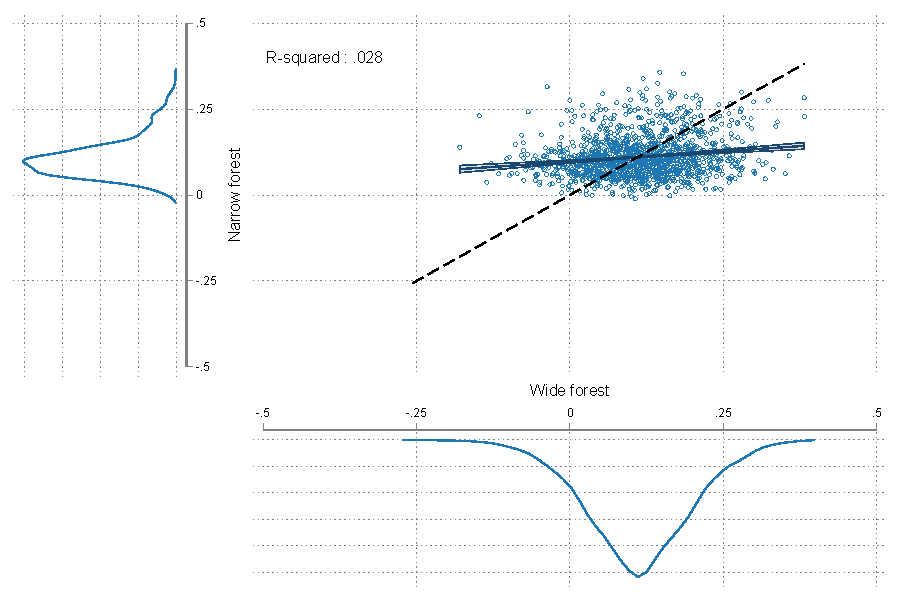
\includegraphics[width=\textwidth]{Figuras/scatter_hist_wide_narrow.pdf}
    \end{subfigure}
    \end{center}
        \footnotesize{This figure plots the relationship between the causal forest conditional ATE estimates from Section \ref{sec:RF} that use the ``wide'' set of covariates (all intake survey responses) and those based on a restricted ``narrow'' set of covariates (age, gender, HS education, and previous borrowing). The scatterplot graphs one estimate versus the other, with the ``wide'' covariate set on the horizontal axis and the ``narrow'' set on the vertical axis. The density plots on each axis show the estimated marginal distribution of conditional ATEs under each covariate set. The density for the ``wide'' covariate set is considerably more dispersed, as the causal forest based on this set of covariates captures considerably more treatment effect heterogeneity.}
    \label{wide_narrow_forests}

%\textit{Do file: } \texttt{wide_narrow_forests.do}       
\end{figure}

\newpage 

\section{Testable Implications of the Exclusion Restriction} \label{sec:testing_exclusion}

%This section describes the testable implications of our exclusion restrictions: \eqref{eq:exclusion0} and \eqref{eq:exclusion1} from Section \ref{sec:potentialOutcomes}. 
%To consider possible violations of these conditions, we require some additional notation.
As above, let $Y_0 \equiv Y(d=0,z=0)$ and $Y_1 \equiv Y(d=1,z=1)$ denote the potential outcomes under \emph{forced treatment}: $Y_0$ is the potential outcome when forced into the status quo contract and $Y_1$ when forced into the commitment contract. 
Further let $Y_{0,2} \equiv Y(d=0,z=2)$ and $Y_{1,2} \equiv Y(d=1,z=2)$ denote the potential outcomes under \emph{free choice of treatment}: $Y_{0,2}$ is the potential outcome when choosing the status quo contract and $Y_{1,2}$ when choosing the commitment contract. 
Using this notation, \eqref{eq:exclusion0} becomes $Y_0 = Y_{0,2}$ and while \eqref{eq:exclusion1} becomes $Y_1 = Y_{1,2}$.
Without imposing these, Assumption \ref{assump:randchoice}(iii) becomes 
\[
Y = \mathbbm{1}(Z =0) Y_{0} + \mathbbm{1}(Z = 1)  Y_{1}  + \mathbbm{1}(Z = 2) \left[(1 - C) Y_{0,2} + C Y_{1,2} \right]
\]
but parts (i) and (ii) continue to hold.
Accordingly, parts (i)--(iii) of Lemma \ref{lem_randchoice} are unchanged, while parts (iv) and (v) become
\[
\mathbbm{E}(Y|D=0,Z=2) = \mathbbm{E}(Y_{0,2}|C=0), \quad
\mathbbm{E}(Y|D=1,Z=2) = \mathbbm{E}(Y_{0,1}|C=1).
\]
Using these expressions, the testable restrictions we consider here are as follows:
\begin{align}
\label{eq:exclusion_append0}
\mathbbm{E}(Y_0|C=0) &= \mathbbm{E}(Y_{0,2}|C=0) \\
\label{eq:exclusion_append1}
\mathbbm{E}(Y_1|C=1) &= \mathbbm{E}(Y_{1,2}|C=1).
\end{align}
%Equation \ref{eq:exclusion_append0} is a restriction on the average potential outcomes of non-choosers that we use to point identify the TUT effect.
%It says that someone who \emph{would} choose the control condition when given a choice, experiences the same potential outcome, on average, when \emph{assigned} to the control condition.
%Equation \ref{eq:exclusion_append1} is a restriction on the average potential outcomes of choosers that we use to point identify the TOT effect.
%It says that someone who \emph{would} choose the commitment contract when given a choice, experiences the same potential outcome, on average, when \emph{assigned} to this condition.
Because they refer to different groups of people--choosers versus non-choosers--either of \eqref{eq:exclusion_append0}  and \eqref{eq:exclusion_append1} could hold when the other is violated.
For this reason we consider each in turn.
Our approach is closely related to arguments from \cite{huber_mellace} and \cite{BinaryRegressor}, among others.
%As such, the following is a heuristic explanation rather than a fully-rigorous proof.
%See the aforementioned papers for more details of how to make this argument fully rigorous.

Consider first \eqref{eq:exclusion_append0}.
Let $p \equiv \mathbbm{P}(C=1) = \mathbbm{P}(D=1|Z=2)$ denote the share of choosers in the population.
This value is point identified regardless of whether the exclusion restriction holds.
Because $Z$ was randomly assigned, a fraction $p$ of borrowers with $Z=0$ are choosers while the remaining $(1-p)$ are non-choosers.
It follows that, regardless of whether the exclusion restriction holds, the observed distribution of $Y|Z=0$ is a mixture of $Y_0|C=0$ and $Y_0|C=1$ with mixing weights $(1-p)$ and $p$.
This allows us to construct a pair of bounds for $\mathbb{E}(Y_0|C=0)$ as follows.
The non-choosers must lie \emph{somewhere} in the distribution of $Y|Z=0$.
Consider the two most extreme possibilities: they could occupy the bottom $(1-p)\times 100\%$ of the distribution or the top $(1-p)\times 100\%$ of the distribution.
For this reason, computing the average of the \emph{truncated} distribution of $Y|Z=0$, cutting out the top $p\times 100\%$, provides a lower bound for the average of $Y_0$ among non-choosers.
Similarly, cutting out the bottom $p \times 100\%$ provides an upper bound.
Let $y^0_{1-p}$ denote the $(1-p)$ quantile of $Y|Z=0$ and $y^0_{p}$ denote the $p$ quantile of the same distribution.
Using this notation, the bounds are given by
\[
\mathbb{E}\left(Y|Z=0, Y\leq y^0_{1-p}\right)\leq \mathbb{E}(Y_0|C=0) \leq \mathbb{E}\left(Y|Z=0, Y \geq y^0_p\right) 
\]
These bounds do not rely on the exclusion restriction.
Under Equation \ref{eq:exclusion_append0}, however, we know that $\mathbb{E}(Y_0|C=0)=\mathbb{E}(Y|D=0,Z=2)$.
Therefore, if the exclusion restriction for non-choosers holds, we must have
\begin{equation}
\mathbb{E}\left(Y|Z=0, Y\leq y^0_{1-p}\right)\leq \mathbb{E}(Y|D=0,Z=2) \leq \mathbb{E}\left(Y|Z=0, Y \geq y^0_p\right).
\label{eq:testable0}
\end{equation}
Equation \ref{eq:testable0} provides a pair of testable implications of \eqref{eq:exclusion_append0}.
If either inequality is violated, then the exclusion restriction for non-choosers fails.
In our experiment, $\widehat{p} = \widehat{\mathbbm{P}}(D=1|Z=2) = 0.11$. For the APR outcome we estimate
\[
\widehat{\mathbbm{E}}(Y_\text{APR}|Z=0,Y_\text{APR}\leq y^0_{0.89}) = 0.48, \quad
\widehat{\mathbbm{E}}(Y_\text{APR}|Z=0, Y_\text{APR}\geq y^0_{0.11}) = 0.62.
\]
Since $\widehat{\mathbbm{E}}(Y_\text{APR}|D=0,Z=2) = 0.58$ falls between these bounds, we find no evidence against the exclusion restriction for non-choosers. 
The same result holds for the financial cost outcome: results available upon request. 
%Repeating this exercise for the financial cost outcome, we see that $\widehat{\mathbbm{E}}(Y_\text{FC}|D=0,Z=2) = 973$ likewise falls between 
%\[
%\widehat{\mathbbm{E}}(Y_\text{FC}|Z=0,Y_\text{FC}\leq y^0_{0.89}) = 626, \quad
%\widehat{\mathbbm{E}}(Y_\text{FC}|Z=0, Y_\text{FC}\geq y^0_{0.11}) = 1046 
%\]
%so we again find no evidence against the exclusion restriction for non-choosers.

We can use an analogous approach to construct testable implications for \ref{eq:exclusion_append1}, yielding 
%Because $Z$ was randomly assigned, a fraction $p$ of participants with $Z = 1$ are choosers so the distribution of $Y|Z=1$ is a mixture of $Y_1|C=1$ and $Y_1|C=0$ with mixing weights $p$ and $1 -p$.
%The participants with $C = 1$ must lie \emph{somewhere} in the distribution of $Y_0|Z=1$ so again consider the two most extreme cases: they could occupy the bottom or the top $p\times 100\%$ of the distribution. 
%\[
%\mathbbm{E}\left(Y|Z=1,Y\leq y^1_{p}\right) \leq \mathbbm{E}(Y_1|C=1) \leq \mathbbm{E}\left(Y|Z=1,Y \geq y^1_{1-p}\right)
%\]
%As above, these bounds do not rely on the exclusion restriction.
%If Equation \ref{eq:exclusion_append1} holds, however, we know that $\mathbb{E}(Y|D=1,Z=2) = \mathbb{E}(Y_1|C=1)$, yielding the following testable implications for choosers
\begin{equation}
\mathbbm{E}\left(Y|Z=1,Y\leq y^1_{p}\right) \leq \mathbbm{E}(Y|D=1,Z=2) \leq \mathbbm{E}\left(Y|Z=1,Y \geq y^1_{1-p}\right).
\label{eq:testable1}
\end{equation}
where $y^1_p$ and $y^1_{1-p}$ are the $p$ and $1 - p$ quantiles of the distribution of $Y|Z=1$.
If either inequality is violated, then the exclusion restriction from Equation \ref{eq:exclusion_append1} fails.
Again, in our experiment $\widehat{p}=0.11$. For the APR outcome we estimate
\[
\widehat{\mathbbm{E}}(Y|Z=1,Y\leq y^1_{0.11}) = 0.06, \quad
\widehat{\mathbbm{E}}(Y|Z=1,Y\geq y^1_{0.89}) = 1.28
\]
Since $\widehat{\mathbbm{E}}(Y_\text{APR}|D=1,Z=2) = 0.43$ falls between these bounds, we find no evidence against the exclusion restriction for the choosers. 
The same holds for the financial cost outcome: results available upon request.
%Repeating this exercise for the financial cost outcome, we see  that $\widehat{\mathbbm{E}}(Y_\text{FC}|D=1,Z=2)= 570$ likewise falls between
%\[
%\widehat{\mathbbm{E}}(Y|Z=1,Y\leq y^1_{0.11}) = 53, \quad
%\widehat{\mathbbm{E}}(Y|Z=1,Y\geq y^1_{0.89}) = 2934
%\]
%so we again find no evidence against the exclusion restriction for the choosers.

%The aforementioned bounds for $\mathbbm{E}(Y_0|C=0)$ and $\mathbbm{E}(Y_1|C=1)$ can alternatively be used construct partial identification bounds for the TOT and TUT effects that do not rely on our exclusion restrictions. If the TOT or TUT expressions from \eqref{eq:TOT} and \eqref{eq:TUT} fall \emph{outside} the partial identification bounds, this is equivalent to finding a violation of \ref{eq:testable0} or \ref{eq:testable1}. We implement these bounds for the TOT and TUT in our companion STATA package.


\section{Estimation and Inference} 
\label{sec:estimation_inference}

\subsection{Regression-based Estimation of TOT, TUT, ASG, ASL, and ASB}

Let $Z_0 \equiv \mathbbm{1}\{Z=0\}$, $Z_1 \equiv \mathbbm{1}\{Z=1\}$, and $Z_2 \equiv \mathbbm{1}\{Z=2\}$.
Under standard regularity conditions, the following proposition shows that an IV regression of $Y$ on an intercept, $Z_1$ and $Z_2 D$ with instruments $(1, Z_0, Z_1)$ provides consistent estimates the ATE and TOT, while an IV regression of $Y$ on an intercept, $-Z_0$ and $-Z_2(1-D)$ with the same instrument set consistently estimates the ATE and TUT effects.

\begin{prop} 
\label{prop:TOTandTUTregs}
Under Assumption \ref{assump:randchoice}, 
\begin{enumerate}[(i)] 
\item $Y = \mathbbm{E}(Y_0) + \text{ATE}\times Z_1 + \text{TOT} \times Z_2 D + U$
\item $Y = \mathbbm{E}(Y_1) + \text{ATE}\times -Z_0 + \text{TUT} \times -Z_2 (1 - D) + V$
\end{enumerate}
where $\mathbbm{E}(U|Z) = \mathbbm{E}(V|Z) = 0$.
\end{prop}

\begin{proof}[Proof of Proposition \ref{prop:TOTandTUTregs}]
For part (i), since $Z_2 D = Z_2 C$ and $(Z_0 + Z_1 + Z_2) = 1$, Assumption \ref{assump:randchoice} (iii) implies $Y= Y_0 + Z_1 (Y_1 - Y_0) + Z_2D(Y_1 - Y_0)$.
Now define 
\[
U \equiv [Y_0 - \mathbbm{E}(Y_0)] + Z_1[(Y_1 - Y_0) - \text{ATE}] + Z_2 D[(Y_1 - Y_0) - \text{TOT}].
\]
Since $Z_2 D = Z_2 C$ and $Z$ is independent of $(Y_1, Y_0)$ by Assumption \ref{assump:randchoice} (i), it follows that $\mathbbm{E}(U|Z) = Z_2 \mathbbm{E}\left[C\left\{(Y_1 - Y_0) - \text{TOT}\right\}|Z\right]$.
Thus, by iterated expectations,
\begin{align*}
\mathbbm{E}\left[C\left\{(Y_1 - Y_0) - \text{TOT}\right\}|Z\right] 
%&=  \mathbbm{P}(C=1|Z) \left[\mathbbm{E}(Y_1 - Y_0|C=1,Z)  - \text{TOT}\right]\\
&= \mathbbm{P}(C=1)\left[\mathbbm{E}(Y_1 - Y_0|C=1) - \text{TOT} \right]=0
\end{align*}
since $Z$ is independent of $(Y_0, Y_1)$ given $C$, an implication of Assumption \ref{assump:randchoice} (i).

For part (ii), since $Z_2(1 - C)= Z_2(1 - D)$ and $(Z_1 + Z_2) = 1 - Z_0$,  Assumption \ref{assump:randchoice} (iii) implies $Y= Y_1 - Z_0 (Y_1 - Y_0) - Z_2(1 - D) (Y_1 - Y_0)$.
Define 
\[
V \equiv [Y_1 - \mathbb{E}(Y_1)] - Z_0[(Y_1 - Y_0) - \text{ATE}] - Z_2(1 - D)[(Y_1 - Y_0) - \text{TUT}].
\]
Since $Z_2(1 - D) = Z_2 (1 - C)$ and $Z$ is independent of $(Y_0, Y_1)$ by Assumption \ref{assump:randchoice} (i),
$\mathbb{E}(V|Z) = -Z_2\mathbb{E}[(1 - C)\left\{(Y_1 - Y_0) - \text{TUT}\right\}|Z]$.
Thus, by iterated expectations,
\begin{align*}
\mathbb{E}[(1 - C)\left\{(Y_1 - Y_0) - \text{TUT}\right\}|Z]
%&= \mathbb{P}(C=0|Z)\left[ \mathbb{E}(Y_1 - Y_0|C=0, Z) - \text{TUT}\right]\\
&= \mathbb{P}(C=0|Z) \left[ \mathbb{E}(Y_1 - Y_0|C=0) - \text{TUT}\right] = 0
\end{align*}
since $Z$ is independent of $(Y_0, Y_1)$ given $C$, an implication of Assumption \ref{assump:randchoice} (i).
\end{proof}

%\begin{prop} 
%\label{prop:TOTreg}
%Under Assumption \ref{assump:randchoice}, $Y = \mathbbm{E}(Y_0) + \text{ATE}\times Z_1 + \text{TOT} \times Z_2 D + U$ where $\mathbbm{E}(U|Z) = 0$.
%\end{prop}
%
%\begin{proof}
%By Assumption \ref{assump:randchoice} (iii),
%$Y= Y_0 + Z_1 (Y_1 - Y_0) + Z_2D(Y_1 - Y_0)$
%%\begin{align*}
%%Y &= Z_0 Y_0 + Z_1 Y_1 + Z_2[(1 - C) Y_0 + CY_1] 
%%= (Z_0 + Z_2)Y_0 + Z_1 Y_1 + Z_2C(Y_1 - Y_0)\\
%%&= (Z_0 + Z_1 + Z_2)Y_0 + Z_1 (Y_1 - Y_0) + Z_2D(Y_1 - Y_0) 
%%= Y_0 + Z_1 (Y_1 - Y_0) + Z_2D(Y_1 - Y_0).
%%\end{align*}
%because $Z_2 D = Z_2 C$ and $(Z_0 + Z_1 + Z_2) = 1$.
%Thus, defining 
%\[
%U \equiv [Y_0 - \mathbbm{E}(Y_0)] + Z_1[(Y_1 - Y_0) - \text{ATE}] + Z_2 D[(Y_1 - Y_0) - \text{TOT}]
%\]
%by construction we have $Y = \mathbbm{E}(Y_0) + \text{ATE} \times Z_1 + \text{TOT} \times Z_2 D+ U$.
%Since $Z_2 D = Z_2 C$ and $Z$ is independent of $(Y_1, Y_0)$ by Assumption \ref{assump:randchoice} (i), we have
%\begin{align*}
%\mathbbm{E}(U|Z) 
%%&= [\mathbbm{E}(Y_0|Z) - \mathbbm{E}(Y_0)]  + Z_1[\mathbbm{E}(Y_1 - Y_0|Z) - \text{ATE}] +  \mathbbm{E}\left[Z_2 D\left\{(Y_1 - Y_0) - \text{TOT}\right\}|Z\right]\\
%%&= [\mathbbm{E}(Y_0) - \mathbbm{E}(Y_0)]  + Z_1[\mathbbm{E}(Y_1 - Y_0) - \text{ATE}] + Z_2 \mathbbm{E}\left[C\left\{(Y_1 - Y_0) - \text{TOT}\right\}|Z\right]\\
%&= Z_2 \mathbbm{E}\left[C\left\{(Y_1 - Y_0) - \text{TOT}\right\}|Z\right].
%\end{align*}
%Finally, by iterated expectations
%\begin{align*}
%\mathbbm{E}\left[C\left\{(Y_1 - Y_0) - \text{TOT}\right\}|Z\right] 
%%&=  \mathbbm{P}(C=1|Z) \left[\mathbbm{E}(Y_1 - Y_0|C=1,Z)  - \text{TOT}\right]\\
%&= \mathbbm{P}(C=1)\left[\mathbbm{E}(Y_1 - Y_0|C=1) - \text{TOT} \right]=0
%\end{align*}
%since $Z$ is conditionally independent of $(Y_0, Y_1)$ given $C$, an implication of \ref{assump:randchoice} (i).
%\end{proof}
%
%%The next proposition provides regression-based estimates of the ATE and TUT.
%\begin{prop}
%\label{prop:TUTreg}
%Under Assumption \ref{assump:randchoice}, $Y = \mathbbm{E}(Y_1) + \text{ATE}\times -Z_0 + \text{TUT} \times -Z_2 (1 - D) + V$ where $\mathbb{E}(V|Z) = 0$.
%Thus, an IV regression of $Y$ on an intercept, $-Z_0$ and $-Z_2(1-D)$ with instruments $(1, Z_0, Z_1)$ provides consistent estimates of the ATE and TUT effects.
%\end{prop}
%
%\begin{proof}
%By Assumption \ref{assump:randchoice} (iii),
%$Y= Y_1 - Z_0 (Y_1 - Y_0) - Z_2(1 - D) (Y_1 - Y_0)$
%%\begin{align*}
%%Y %&= Z_0 Y_0 + Z_1 Y_1 + Z_2[(1 - C) Y_0 + CY_1] 
%%&= Z_0 Y_0 + Z_1 Y_1 + Z_2[(1 - C) (Y_0 - Y_1) + Y_1]
%%&= Z_0 Y_0 + (Z_1 + Z_2) Y_1 + Z_2(1 - C) (Y_0 - Y_1) = Z_0 Y_0 + (1 - Z_0) Y_1 + Z_2(1 - D) (Y_0 - Y_1) \\
%%= Y_1 - Z_0 (Y_1 - Y_0) - Z_2(1 - D) (Y_1 - Y_0)
%%\end{align*}
%since $Z_2(1 - C)= Z_2(1 - D)$ and $(Z_1 + Z_2) = 1 - Z_0$.
%Thus, defining 
%\[
%V \equiv [Y_1 - \mathbb{E}(Y_1)] - Z_0[(Y_1 - Y_0) - \text{ATE}] - Z_2(1 - D)[(Y_1 - Y_0) - \text{TUT}]
%\]
%by construction we have $Y = \mathbb{E}(Y_1) + \text{ATE} \times -Z_0 + \text{TUT} \times -Z_2(1 - D) + V$.
%Now, since $Z_2(1 - D) = Z_2 (1 - C)$ and $Z$ is independent of $(Y_0, Y_1)$ by Assumption \ref{assump:randchoice} (i),
%\begin{align*}
%\mathbb{E}(V|Z) 
%%&= [\mathbb{E}(Y_1|Z) - \mathbb{E}(Y_1)] - Z_0[\mathbb{E}(Y_1 - Y_0|Z) - \text{ATE}] - \mathbb{E}[Z_2(1 - D)\left\{(Y_1 - Y_0) - \text{TUT}\right\}|Z]\\
%%&= [\mathbb{E}(Y_1) - \mathbb{E}(Y_1)] - Z_0[\mathbb{E}(Y_1 - Y_0) - \text{ATE}] - Z_2\mathbb{E}[(1 - C)\left\{(Y_1 - Y_0) - \text{TUT}\right\}|Z]\\
%&= -Z_2\mathbb{E}[(1 - C)\left\{(Y_1 - Y_0) - \text{TUT}\right\}|Z].
%\end{align*}
%Finally, by iterated expectations,
%\begin{align*}
%\mathbb{E}[(1 - C)\left\{(Y_1 - Y_0) - \text{TUT}\right\}|Z]
%%&= \mathbb{P}(C=0|Z)\left[ \mathbb{E}(Y_1 - Y_0|C=0, Z) - \text{TUT}\right]\\
%&= \mathbb{P}(C=0|Z) \left[ \mathbb{E}(Y_1 - Y_0|C=0) - \text{TUT}\right] = 0
%\end{align*}
%since $Z$ is independent of $(Y_0, Y_1)$ given $C$, an implication of Assumption \ref{assump:randchoice} (i).
%\end{proof}

Since $\text{ASG} = \text{TOT} - \text{TUT}$, the preceding proposition provides a consistent estimate of the $\text{ASG}$ effect.
The $\text{ASB}$ effect, $\mathbbm{E}(Y_0|C=1) - \mathbb{E}(Y_0|C=0)$, can likewise be estimated by taking the difference of coefficients across two linear IV regressions with \emph{no intercept} and instrument sets $(Z_0, Z_2)$, as shown in the following proposition.

\begin{prop}
\label{prop:ASBreg}
Under Assumption \ref{assump:randchoice}
\begin{enumerate}[(i)]
    \item $(1 - D) Y = \mathbbm{E}(Y_{0}) \times Z_0 + \mathbbm{E}(Y_{0}|C=0) \times (1 - D)Z_2 + U_{0}$
    \item  $(1 - D) Y = \mathbbm{E}(Y_{0}) \times(Z_0 + Z_2) + \mathbbm{E}(Y_{0}|C=1)\times -DZ_2 + U_{1}$
\end{enumerate}
where $\mathbbm{E}(U_0|Z) = \mathbbm{E}(U_1|Z) = 0$.
%Thus, an IV regression of $(1 - D)Y$ on $Z_0$ and $(1 - D)Z_2$ with instruments $(Z_0, Z_2)$ and no intercept consistently estimates $\mathbb{E}(Y_0)$ and $\mathbb{E}(Y_0|C=0)$. 
%Similarly, an IV regression of $(1 - D)Y$ on $(Z_0 + Z_2)$ and $-DZ_2$ with instruments $(Z_0, Z_2)$ and no intercept consistently estimates $\mathbb{E}(Y_0)$ and $\mathbb{E}(Y_0|C=1)$.
\end{prop}

\begin{proof}
Assumption \ref{assump:randchoice} (ii) implies $(1 - D) = Z_0 + Z_2(1 - C)$. Hence, 
\begin{align*}
(1 - D)Y 
%&=  [Z_0 + Z_2 (1 - C)]\left\{Z_0 Y_0 + Z_1 Y_1 + Z_2[(1 - C) Y_0 + CY_1]\right\}\\
&= Z_0 Y_0 + Z_2 (1 - C) [(1 - C) Y_0 + C Y_1] = Z_0 Y_0 + Z_2 (1 - C) Y_0
\end{align*}
by Assumption \ref{assump:randchoice} (iii), since $Z_j^2 = Z_j$ for any $j$ and $Z_j Z_k = 0$ for any $j \neq k$ and, similarly, $(1 - C)^2 = (1 - C)$ and $C (1 - C) = 0$.
Therefore, since $Z_2 (1 - C) = Z_2 (1 - D)$,
\[
(1 - D)Y = Z_0 Y_0 + Z_2 (1 - D) Y_0, \quad
(1 - D)Y = (Z_0 + Z_2) Y_0 + (-DZ_2) Y_0. 
\]
Now, define 
\begin{align*}
U_0 &\equiv Z_0 [Y_0 - \mathbbm{E}(Y_0)] + Z_2(1 - D)[Y_0 - \mathbbm{E}(Y_0|C=0)]\\
U_1 &\equiv (Z_0 + Z_2)[Y_0 - \mathbbm{E}(Y_0)] + (-Z_2 D)[Y_0 - \mathbbm{E}(Y_0|C=1)].
\end{align*}
%by construction, we have
%\begin{align*}
%Y &= \mathbbm{E}(Y_0) \times Z_0 + \mathbbm{E}(Y_0|C=0) \times Z_2(1 - D) + U_0\\
%Y &= \mathbbm{E}(Y_0) \times (Z_0 + Z_2)+ \mathbbm{E}(Y_0|C=1) (-Z_2D) + U_1.
%\end{align*}
Since $Z_2(1-D) = Z_2(1 - C)$, and $Z$ is independent of $Y_0$,  
\begin{align*}
\mathbbm{E}(U_0|Z) 
%&= Z_0[\mathbbm{E}(Y_0|Z) - \mathbbm{E}(Y_0)] + Z_2\mathbbm{E}\{(1 - C) [Y_0 - \mathbbm{E}(Y_0|C=0) |Z\}\\
&= Z_2 \mathbbm{E}[Y_0 - \mathbbm{E}(Y_0|C=0) | C = 0, Z] = 0
\end{align*}
by iterated expectations and the fact that $Z$ is conditionally independent of $Y_0$ given $C$. 
Since $Z_2 D = Z_2 C$, a nearly identical argument gives
\begin{align*}
\mathbbm{E}(U_1|Z) 
%&= (Z_0 + Z_2)[Y_0 - \mathbbm{E}(Y_0|Z)] -Z_2\mathbbm{E}\{C [Y_0 - \mathbbm{E}(Y_0|C=1) |Z\}\\
&= -Z_2 \mathbbm{E}[Y_0 - \mathbbm{E}(Y_0|C=0) | C = 1, Z] = 0. \qedhere
\end{align*}
\end{proof}


The final result in this section implies that the $\text{ASL}$ effect, $\mathbbm{E}(Y_1|C=1) - \mathbb{E}(Y_1|C=0)$, can be estimated as the difference of coefficients across two linear IV regressions with \emph{no intercept} and instrument set $(Z_1, Z_2)$.

\begin{prop}
\label{prop:ASLreg}
Under Assumption \ref{assump:randchoice},
\begin{enumerate}[(i)]
\item $D Y = \mathbbm{E}(Y_{1}) \times(Z_1 + Z_2) + \mathbbm{E}(Y_{1}|C=0)\times (D - 1)Z_2 + V_{0}$
\item  $D Y = \mathbbm{E}(Y_{1}) \times Z_1 + \mathbbm{E}(Y_{1}|C=1)\times D Z_2+ V_{1}$
\end{enumerate}
where $\mathbbm{E}(V_0|Z) = \mathbbm{E}(V_1|Z) = 0$.
\end{prop}


\begin{proof}
By Assumption \ref{assump:randchoice}, $D = Z_1 + Z_2 C$. Hence, by Assumption \ref{assump:randchoice} (iii),
\begin{align*}
DY 
%&=  (Z_1 + Z_2 C)\left\{Z_0 Y_0 + Z_1 Y_1 + Z_2[(1 - C) Y_0 + CY_1]\right\}\\
&= Z_1 Y_1 + Z_2 C[(1 -C) Y_0 + C Y_1] = Z_1 Y_1 + Z_2 C Y_1
\end{align*}
because $Z_j^2 = Z_j$ for any $j$ and $Z_j Z_k = 0$ for any $j \neq k$ and, similarly, $(1 - C)^2 = (1 - C)$ and $C (1 - C) = 0$. Therefore, since $Z_2 (1 - C) = Z_2 (1 - D)$,
\[
 DY = (Z_1 + Z_2)Y_1 + Z_2 (D - 1) Y_1, \quad
 DY = Z_1 Y_1 + Z_2 D Y_1.
\]
Now, define
\begin{align*}
V_0 &= (Z_1 + Z_2)[Y_1 - \mathbbm{E}(Y_1)] + Z_2(D - 1)[Y_1 - \mathbbm{E}(Y_1|C=0)]\\
V_1 &= Z_1[Y_1 - \mathbbm{E}(Y_1)] + Z_2D[Y_1 - \mathbbm{E}(Y_1|C=1)].
\end{align*}
%by construction we have
%\begin{align*}
%Y &= \mathbbm{E}(Y_1) \times (Z_1 + Z_2) + \mathbbm{E}(Y_1 | C = 0) \times Z_2 (D - 1) + V_0\\
%Y &= \mathbbm{E}(Y_1) \times Z_1 + \mathbbm{E}(Y_1 | C = 1) \times Z_2 D + V _1.
%\end{align*}
Since $Z_2(1 - D) = Z_2(1 - C)$ and $Z$ is independent of $Y_1$,
\begin{align*}
\mathbbm{E}(V_0|Z) 
%&= (Z_1 + Z_2) [\mathbbm{E}(Y_1|Z) - \mathbbm{E}(Y_1) ]  - Z_2 \mathbbm{E}\{(1 - C)  [Y_1 - \mathbbm{E}(Y_1 | C=0)|Z\} \\
&= -Z_2 \mathbbm{E}[Y_1 - \mathbbm{E}(Y_1 | C=0)|C=0, Z] = 0
\end{align*}
by iterated expectations and the fact that  $Z$ is conditionally independent of $Y_1$ given $C$. 
Since $Z_2 D = Z_2 C$, a similar argument gives
\begin{align*}
\mathbbm{E}(V_1|Z) 
%&= Z_1 [\mathbbm{E}(Y_1 | Z) - \mathbbm{E}(Y_1)]  + Z_2 \mathbbm{E}\{C  [Y_1 - \mathbbm{E}(Y_1 | C=1)|Z\} \\
&= Z_2 \mathbbm{E}[Y_1 - \mathbbm{E}(Y_1 | C=1)|C=1, Z] = 0. \qedhere
\end{align*}
\end{proof}

\normalsize
%Really force it to normal size and linespread
\normalsize


\subsection{Inference for ASG, ASB, and ASL}
\label{subsec:inference}

We now explain how to carry out cluster-robust inference for the ASG, ASB, and ASL effects, as implemented in our companion STATA package.
Each of these effects can be expressed as a difference of coefficients from two just-identified linear IV regressions.
The ASG effect is the difference of the \text{TOT} and \text{TUT} effects from Proposition \ref{prop:TOTandTUTregs}. 
Similarly, the ASB effect is the difference of $\mathbb{E}(Y_0|C=1)$ and $\mathbbm{E}(Y_0|C=0)$ from Proposition \ref{prop:ASBreg} while the ASL effect is the difference of $\mathbbm{E}(Y_1|C=1)$ and $\mathbbm{E}(Y_1|C=0)$ from Proposition \ref{prop:ASLreg}.
Within each pair of IV regressions the outcome variable and instrument set is identical; only the regressors differ. 
Since our estimators of all three effects share the same structure, our discussion abstracts from the specific regressors and instruments used in each case.

Let $g = 1, ..., G$ index clusters and $i = 1, ..., N_g$ index individuals within a particular cluster $g$. 
In our experiment, a cluster is a branch-day combination and the experimentally-assigned treatment (control, forced, or choice arm) is assigned at the cluster level.
We assume that observations are iid across clusters but potentially correlated within cluster.
Now consider a pair of just-identified linear IV regressions given by
$Y_{ig} = \boldsymbol{X}_{1,ig}' \boldsymbol{\theta}_0 + U_{ig}$ and $Y_{ig} = \boldsymbol{X}_{0,ig}' \boldsymbol{\theta}_1 + V_{ig}$ with common instrument vector $\boldsymbol{W}_{ig}$. 
Stacking observations in the usual manner, e.g.\
$\mathbf{W}_g' \equiv \begin{bmatrix}
\boldsymbol{W}_{1g} & \cdots & 
\boldsymbol{W}_{N_gg} 
\end{bmatrix}$ and 
$\mathbf{W}' = \begin{bmatrix}
\mathbf{W}_1' & \cdots & \mathbf{W}_G'
\end{bmatrix}$
we can write the preceding equations in matrix form as $\mathbf{Y} = \mathbf{X}_1\boldsymbol{\theta_1} + \mathbf{U}$ and $\mathbf{Y} = \mathbf{X}_0\boldsymbol{\theta_0} + \mathbf{V}$ with instrument matrix $\mathbf{W}$.
Now, the IV estimators for $\boldsymbol{\theta}_1$ and $\boldsymbol{\theta}_0$ can be expressed as 
\begin{align*}
\widehat{\boldsymbol{\theta}}_1 
&= \left(\mathbf{W}'\mathbf{X}_1\right)^{-1}\mathbf{W}'\mathbf{Y}  = \boldsymbol{\theta}_1 + \left(\mathbf{W}'\mathbf{X}_1\right)^{-1}\mathbf{W}'\mathbf{U}\\ 
\widehat{\boldsymbol{\theta}}_0 
&= \left(\mathbf{W}'\mathbf{X}_0\right)^{-1}\mathbf{W}'\mathbf{Y} = \boldsymbol{\theta}_0 + \left(\mathbf{W}'\mathbf{X}_0\right)^{-1}\mathbf{W}'\mathbf{V}.
\end{align*}

%Our parameter of interest is an element of the difference $(\theta_1 - \theta_0)$, so it suffices to estimate the asymptotic variance of $(\widehat{\boldsymbol{\theta}}_1 - \widehat{\boldsymbol{\theta}}_0)$.
%Re-arranging the preceding two equations, 
%\begin{align*}
%\sqrt{G} \left(\widehat{\boldsymbol{\theta}}_1  - \boldsymbol{\theta}_1\right) &= 
% \left(\frac{\mathbf{W}'\mathbf{X}_1}{G}\right)^{-1}\left(\frac{\mathbf{W}'\mathbf{U}}{\sqrt{G}}\right) = \left( \frac{1}{G} \sum_{g=1}^G \mathbf{W}_g' \mathbf{X}_{1,g}\right)^{-1}\left(\frac{1}{\sqrt{G}} \sum_{g=1}^G\mathbf{W}_g' \mathbf{U}_g\right) \\ 
%\sqrt{G} \left(\widehat{\boldsymbol{\theta}}_0  - \boldsymbol{\theta}_0\right) &= 
% \left(\frac{\mathbf{W}'\mathbf{X}_0}{G}\right)^{-1}\left(\frac{\mathbf{W}'\mathbf{V}}{\sqrt{G}}\right) = \left( \frac{1}{G} \sum_{g=1}^G \mathbf{W}_g' \mathbf{X}_{0,g}\right)^{-1}\left(\frac{1}{\sqrt{G}} \sum_{g=1}^G\mathbf{W}_g' \mathbf{V}_g\right).
%\end{align*}
%Now, define $\mathbf{Q}_0 \equiv \mathbb{E}[\mathbf{W}_g'\mathbf{X}_{0g}]$ and $\mathbf{Q}_1 \equiv \mathbb{E}[\mathbf{W}_g'\mathbf{X}_{1g}]$ and suppose that these expectations exist and that the matrices $\mathbf{Q}_0$ and $\mathbf{Q}_1$ are invertible. Then, as $G \rightarrow \infty$
%\[
% \left( \frac{1}{G} \sum_{g=1}^G \mathbf{W}_g' \mathbf{X}_{0,g}\right)^{-1} \rightarrow_p \mathbf{Q}_0^{-1}, \quad
% \left( \frac{1}{G} \sum_{g=1}^G \mathbf{W}_g' \mathbf{X}_{1,g}\right)^{-1} \rightarrow_p \mathbf{Q}_1^{-1} \quad
%\]
%by the continuous mapping theorem.
By our experimental design and exclusion restriction, $\mathbf{W}_{ig}$ is independent of $U_{ig}$ both unconditionally and conditional on cluster size. 
%Therefore,
%\begin{align*}
%\mathbb{E}[\mathbf{W}_g' \mathbf{U}_g] &=  \mathbb{E}\left[ \sum_{i=1}^{N_g} \mathbf{W}_{ig} U_{ig} \right] = \mathbb{E}_{N_g}\left[ \mathbb{E}\left\{\left. \sum_{i=1}^{N_g} \mathbf{W}_{ig} U_{ig} \right| N_g \right\}\right]\\
%&= \mathbb{E}_{N_g}\left[ \sum_{i=1}^{N_g} \mathbb{E}(\mathbf{W}_{ig} U_{ig}|N_g)\right] = \mathbb{E}_{N_g}\left[ \sum_{i=1}^{N_g} \mathbb{E}(\mathbf{W}_{ig}U_{ig})\right] = 0
%\end{align*}
%by iterated expectations, and similarly smilarly, $\mathbb{E}[\mathbf{W}_g'\mathbf{V}_g] = \mathbf{0}$. 
%Thus, under mild regularity conditions (e.g.\ finite fourth moments), as $G \rightarrow \infty$  we have
%\[
%\frac{1}{\sqrt{G}} \sum_{g=1}^G \mathbf{W}_g' \otimes \begin{bmatrix} \mathbf{U}_g \\ \mathbf{V}_g \end{bmatrix} \rightarrow_d \text{N}(\mathbf{0}, \boldsymbol{\Omega})
%\]
%where the heteroskedasticity-- and cluster--robust variance-covariance matrix $\boldsymbol{\Omega}$ is 
%\[
%\boldsymbol{\Omega} \equiv 
% \mathbb{E} \left[\left(\mathbf{W}_g \mathbf{W}_g' \right)\otimes \begin{pmatrix}
%\mathbf{U}_g \mathbf{U}_g' & \mathbf{U}_g \mathbf{V}_g' \\
%\mathbf{V}_g \mathbf{U}_g' & \mathbf{V}_g \mathbf{V}_g'  
%\end{pmatrix} \right] \equiv \begin{bmatrix}
%\Omega_{UU} & \Omega_{UV} \\
%\Omega_{VU} & \Omega_{VV}
%\end{bmatrix}.
%\]
%Therefore, the joint limiting distribution of $\widehat{\boldsymbol{\theta}}_1$ and $\widehat{\boldsymbol{\theta}}_0$ is given by
%\[
%\begin{bmatrix}
%\sqrt{G}(\widehat{\boldsymbol{\theta}}_1 - \boldsymbol{\theta}_1)\\
%\sqrt{G}(\widehat{\boldsymbol{\theta}}_0 - \boldsymbol{\theta}_0)
%\end{bmatrix} \rightarrow_d
%\begin{bmatrix}
%\mathbf{Q}_1^{-1} & \mathbf{0} \\
%\mathbf{0} & \mathbf{Q}_0^{-1} 
%\end{bmatrix}
%\begin{bmatrix}
%\boldsymbol{\xi}_U \\ \boldsymbol{\xi}_V 
%\end{bmatrix}, \quad
%\begin{bmatrix}
%\boldsymbol{\xi}_U \\ \boldsymbol{\xi}_V 
%\end{bmatrix} \sim \text{N}\left(\begin{bmatrix} \mathbf{0} \\ \mathbf{0}\end{bmatrix},
%\begin{bmatrix}
%\Omega_{UU} & \Omega_{UV} \\
%\Omega_{VU} & \Omega_{VV}
%\end{bmatrix}\right)
%\]
%from which it follows by the continuous mapping theorem that
%\[
%\sqrt{G}\left[ (\widehat{\boldsymbol{\theta}}_1 - \widehat{\boldsymbol{\theta}}_0 ) - (\boldsymbol{\theta}_1 - \boldsymbol{\theta}_0)\right] 
%\rightarrow_d
%\begin{bmatrix}
%\mathbf{Q}_1^{-1} & -\mathbf{Q}_0^{-1}
%\end{bmatrix}
%\begin{bmatrix}
%\boldsymbol{\xi}_U \\ \boldsymbol{\xi}_V 
%\end{bmatrix}.
%\]
%To use this result in practice, we estimate the standard errors of  $(\widehat{\boldsymbol{\theta}}_1 - \widehat{\boldsymbol{\theta}}_0)$ as the square root of the diagonal elements of the matrix
Hence, by a standard argument and under mild regularity conditions, the following expression provides a consistent, cluster robust estimator of $\widehat{\text{Avar}}(\widehat{\boldsymbol{\theta}}_1 - \widehat{\boldsymbol{\theta}}_0)$ 
\[
\widehat{\text{Avar}}(\widehat{\boldsymbol{\theta}}_1 - \widehat{\boldsymbol{\theta}}_0) 
= \begin{bmatrix}
\left(\mathbf{W}'\mathbf{X}_1\right)^{-1} &
-\left(\mathbf{W}'\mathbf{X}_0\right)^{-1} 
\end{bmatrix}
\begin{bmatrix}
\mathbf{S}_{UU}& \mathbf{S}_{UV}\\
\mathbf{S}_{UV}'& \mathbf{S}_{VV}
\end{bmatrix} 
\begin{bmatrix}
\left(\mathbf{X}_1'\mathbf{W}\right)^{-1} \\
-\left(\mathbf{X}_0'\mathbf{W}\right)^{-1} 
\end{bmatrix}
\]
where we define the IV residuals
$\widehat{\mathbf{U}}_g \equiv \mathbf{Y}_g - \mathbf{X}_{1,g}\widehat{\boldsymbol{\theta}}_1$ and
$\widehat{\mathbf{V}}_g \equiv \mathbf{Y}_g - \mathbf{X}_{0,g}\widehat{\boldsymbol{\theta}}_0$ along with the matrices
$\mathbf{S}_{UU} \equiv \sum_{g=1}^G \mathbf{W}_g' \widehat{\mathbf{U}}_g \widehat{\mathbf{U}}_g' \mathbf{W}_g$,
$\mathbf{S}_{UV} \equiv \sum_{g=1}^G \mathbf{W}_g' \widehat{\mathbf{U}}_g \widehat{\mathbf{V}}_g' \mathbf{W}_g$, and finally
$\mathbf{S}_{VV} \equiv \sum_{g=1}^G \mathbf{W}_g' \widehat{\mathbf{V}}_g \widehat{\mathbf{V}}_g' \mathbf{W}_g$.
In our application the number of clusters, $G$, is large.
If desired, an \emph{ad hoc} degrees of freedom correction can be applied by multiplying the associated standard errors by $\sqrt{G/(G-1)}$.


\end{appendix}

\end{document}
